\documentclass{beamer}
\usepackage[utf8]{inputenc}
\usetheme{Madrid}
\usecolortheme{seahorse}
\setbeamertemplate{caption}[numbered]

\title{Una Introducción al Aprendizaje de Máquina asistido por R y Python}
\author[iprea@udistrital.edu.co]{Luis Alejandro Masmela-Caita\\
Laura Camila Vergara-González\\
Wilson Eduardo Jeréz-Hernández}
\date{Noviembre de 2023}

\begin{document}
	
	\frame{\titlepage}
	
	
	\begin{frame}
		\frametitle{Modelo de Aprendizaje de Máquina}
						\begin{block}{Modelo vs Algoritmo}	
		\begin{itemize}
			\item \textbf{¿Qué es un modelo?} \textit{Un modelo es cualquier tipo de función que tiene capacidad predictiva.}
			\item\textbf{¿Qué es un algoritmo?}\textit{Un algoritmo es un conjunto de pasos realizados en orden  con el objetivo de realizar una tarea o resolver un problema específico.}
			\item Un \textbf{Modelo de Aprendizaje de Máquina} es el resultado del proceso de entrenar un algoritmo con un conjunto de datos.
		\end{itemize}
	\end{block}
	\end{frame}
	
	
	\begin{frame}
	\frametitle{Modelo de Aprendizaje de Máquina}
\textit{\textbf{``Todos los modelos son erroneos, pero algunos son útiles."}}
	\begin{figure}
		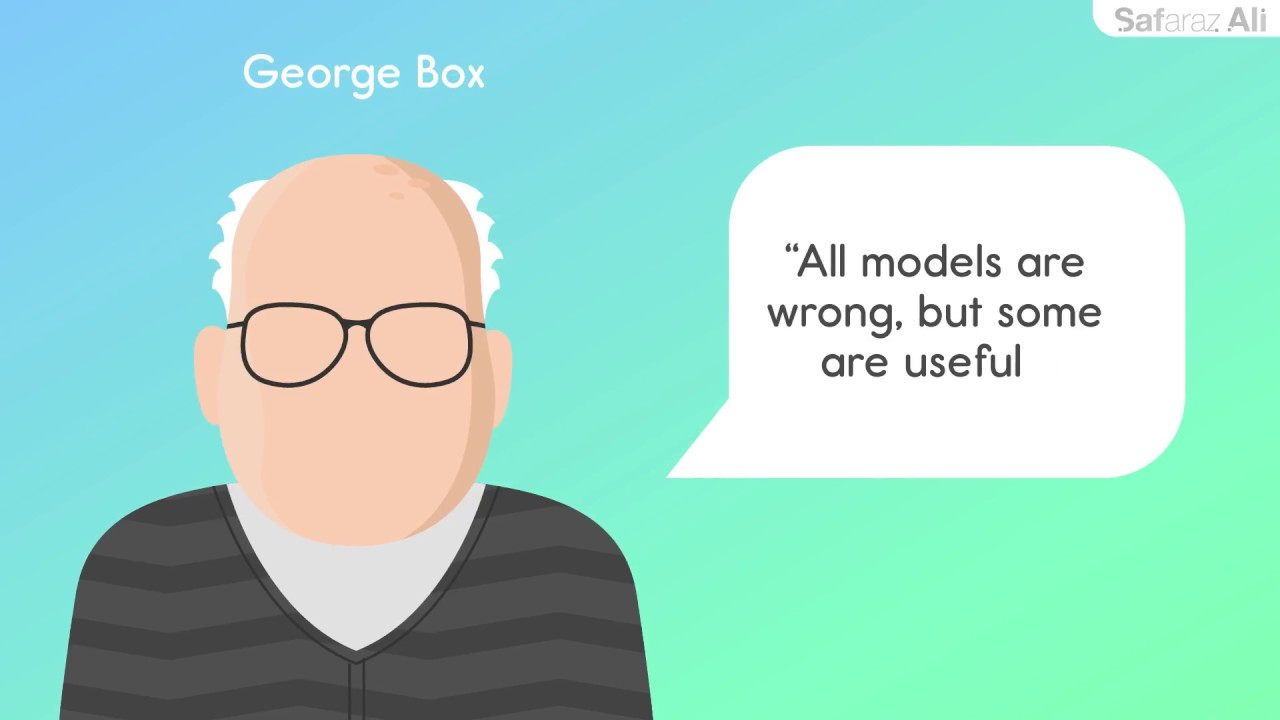
\includegraphics[width=0.7\textwidth]{Box_imagen.jpg}
		\caption{https://www.youtube.com/@SafarazAli}
	\end{figure}
	\end{frame}
	
	
		\begin{frame}
		\frametitle{Modelo de Aprendizaje de Máquina}
		\textit{\textbf{``La verdad es demasiado complicada como para permitir algo más que una aproximación."}}
		\begin{figure}
			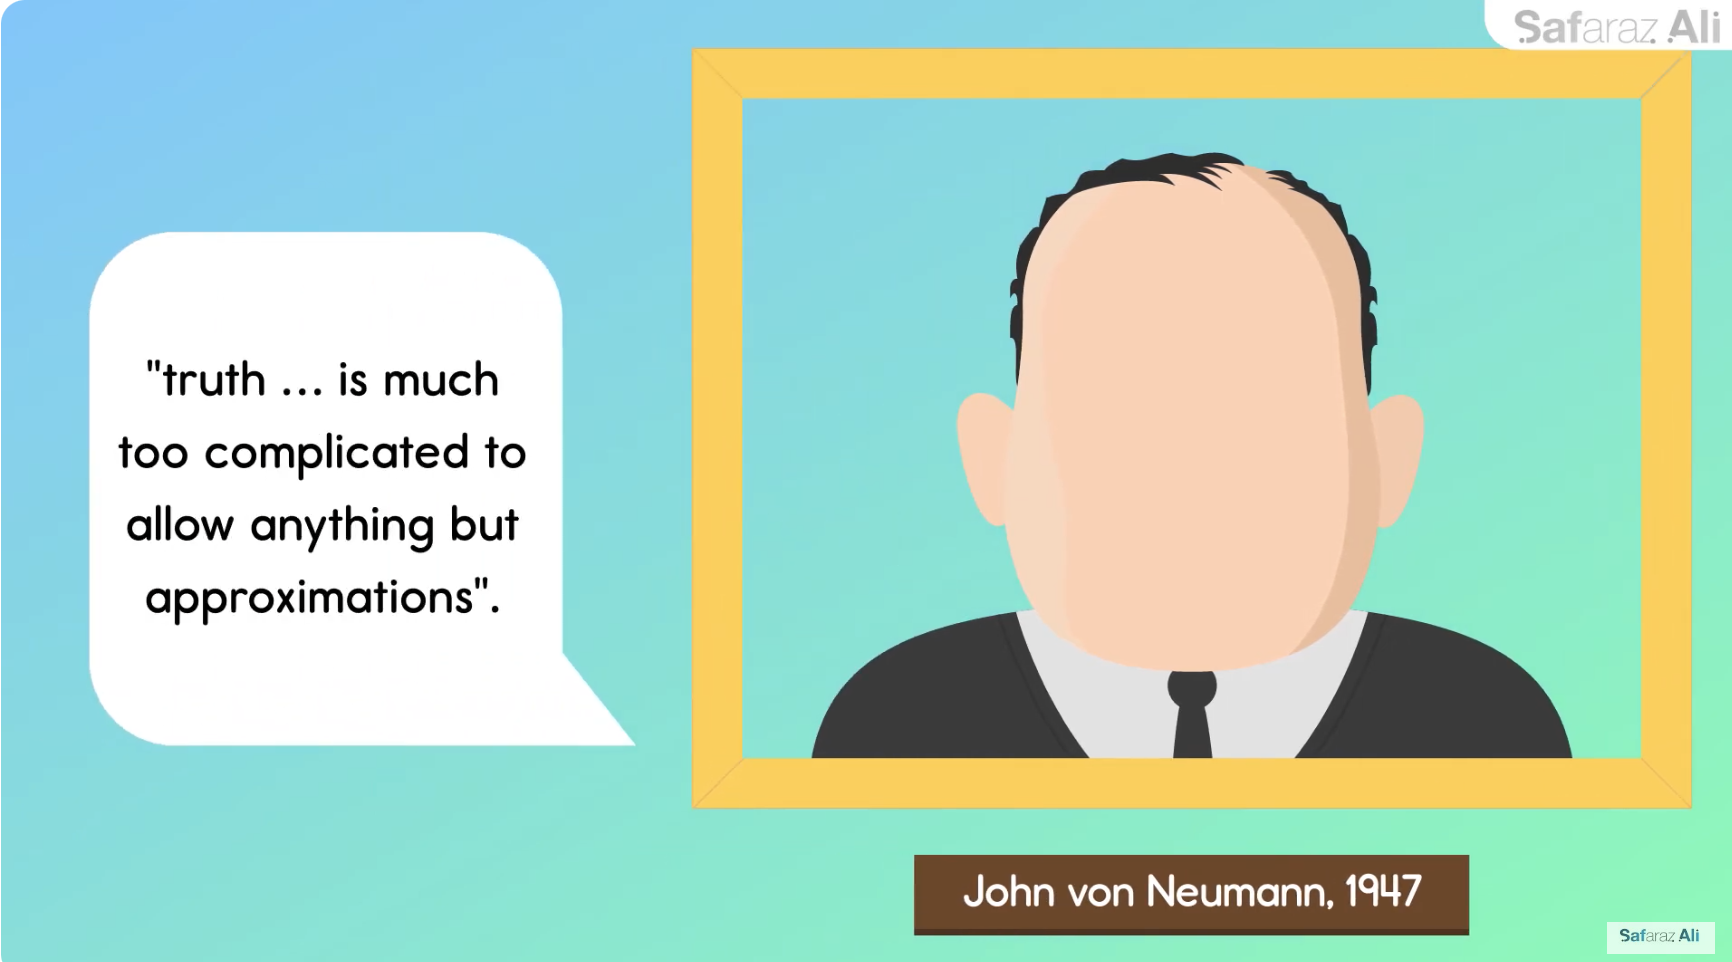
\includegraphics[width=0.7\textwidth]{Von_Newman_imagen}
			\caption{https://www.youtube.com/@SafarazAli}
		\end{figure}
	\end{frame}
	
	
	\begin{frame}
		\frametitle{En Resumen}
		\begin{itemize}
			\item El \textbf{algoritmo} es como las instrucciones para construir una máquina de predicción.
			\item El \textbf{modelo} es la máquina ya construida y entrenada para realizar una tarea específica.
		\end{itemize}
	\end{frame}
	

	

	\begin{frame}{Modelos de Aprendizaje de Máquina}
\begin{block}{El Problema}
	\begin{figure}
		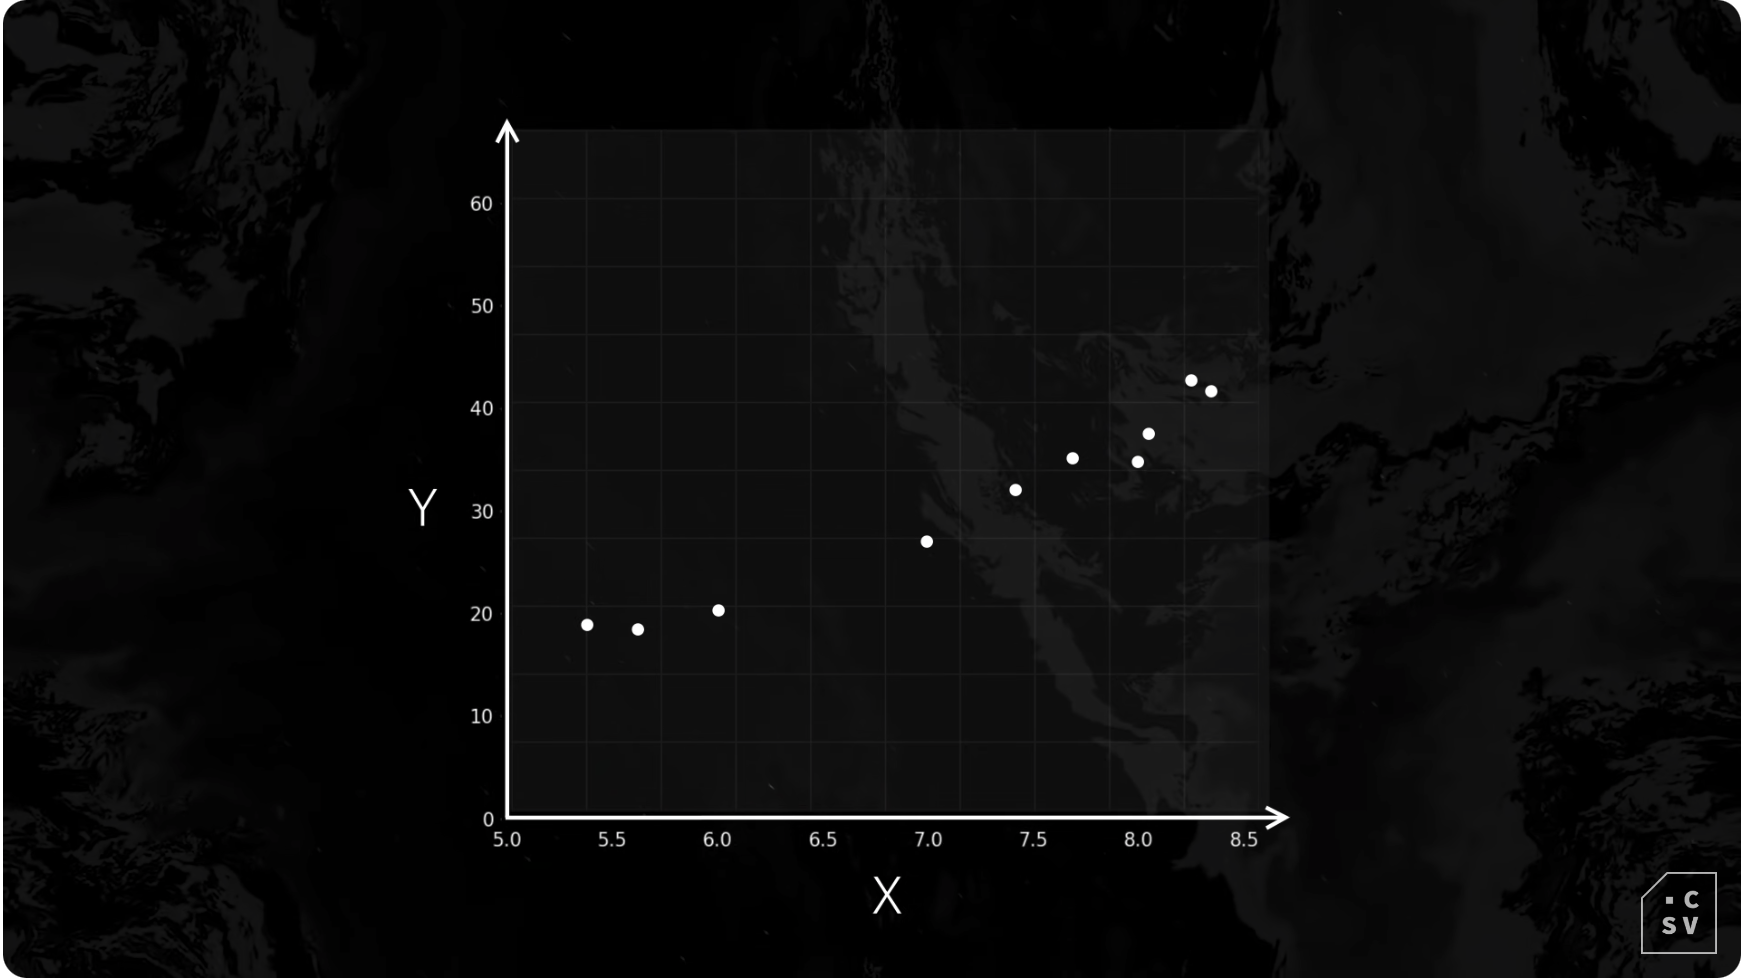
\includegraphics[width=0.7\textwidth]{modelo-algoritmo_1}
		\caption{https://www.youtube.com/}
		\centering
	\end{figure}
\end{block}
		
	\end{frame}
	
		\begin{frame}{Modelos de Aprendizaje de Máquina}
		\begin{block}{El Modelo}
			\begin{figure}
				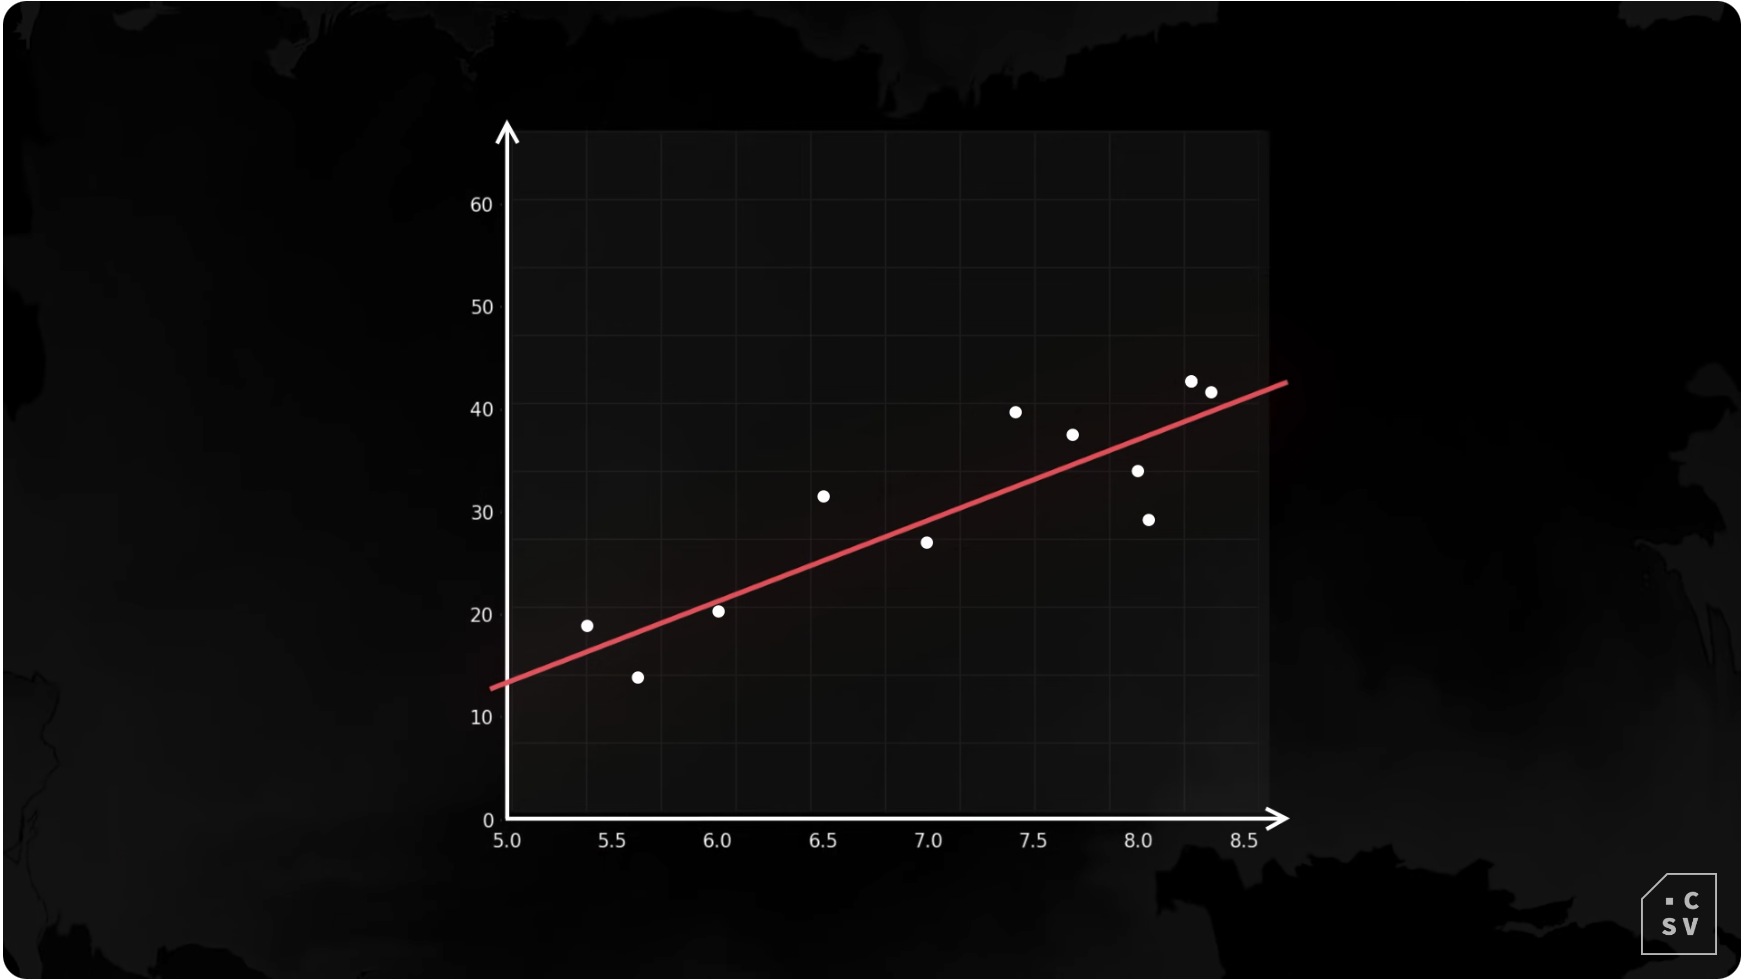
\includegraphics[width=0.7\textwidth]{modelo-algoritmo_2}
				\caption{https://www.youtube.com/}
				\centering
			\end{figure}
		\end{block}
		
	\end{frame}
	
		\begin{frame}{Modelos de Aprendizaje de Máquina}
		\begin{block}{El Algoritmo}
			\begin{figure}
				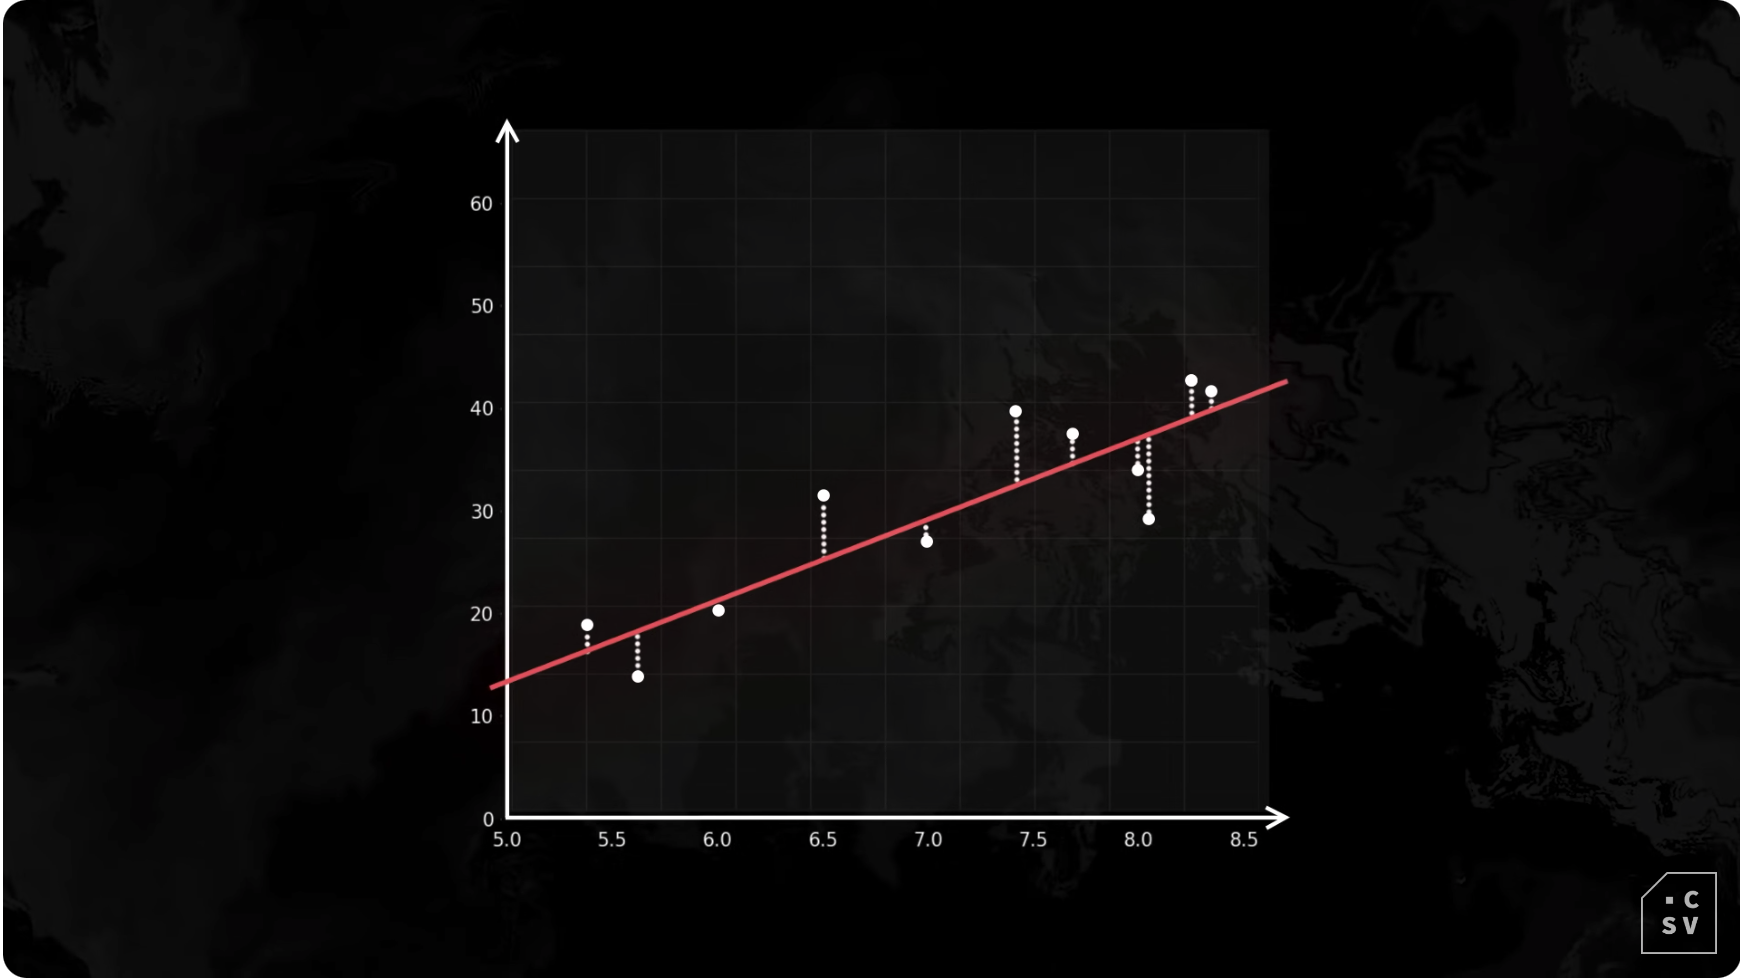
\includegraphics[width=0.7\textwidth]{modelo-algoritmo_3}
				\caption{https://www.youtube.com/}
				\centering
			\end{figure}
		\end{block}
		
	\end{frame}

	

\begin{frame}
	\frametitle{Conceptos en Aprendizaje de Máquina}
			\begin{block}{El Conjunto de Datos}
	\begin{itemize}
		\item \textbf{Características (Features)}:
		\begin{itemize}
			\item Representan las entradas o datos de entrada en un modelo de Machine Learning.
			\item Son las variables o atributos que se utilizan para hacer predicciones.
			\item Ejemplos: píxeles de una imagen, palabras en un documento, mediciones en un conjunto de datos.
		\end{itemize}			
		\item \textbf{Etiquetas (Labels)}:
		\begin{itemize}
			\item Representan las salidas o resultados deseados en un modelo de Machine Learning.
			\item Son las respuestas que el modelo debe aprender a predecir.
			\item Ejemplos: categorías de imágenes (perro, gato), clasificación de texto (positivo, negativo), valor numérico de una propiedad.
		\end{itemize}
		\item \textbf{Ejemplos (Examples)}: son instancias de datos utilizadas para entrenar y evaluar modelos de aprendizaje automático.
	\end{itemize}
		\end{block}
\end{frame}


	\begin{frame}
	\frametitle{Conceptos en Aprendizaje de Máquina}
	\begin{figure}
		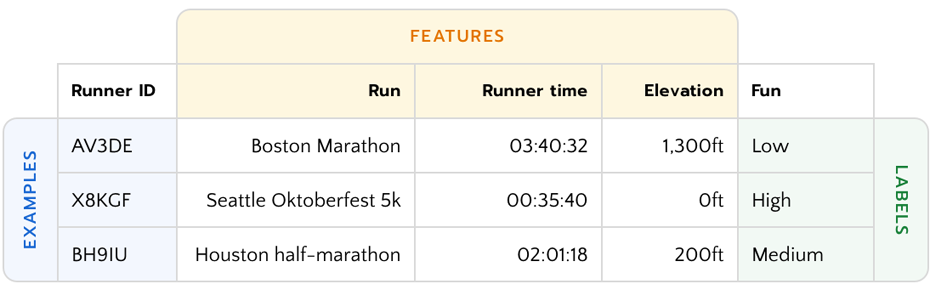
\includegraphics[width=0.9\textwidth]{labels_features}
		\caption{https://pair.withgoogle.com/chapter/data-collection/}
		\centering
	\end{figure}
\begin{block}{}
El dataframe anterior contiene datos sobre carreras que una aplicación podría usar para entrenar un modelo de aprendizaje automático para predecir qué tan divertida será una carrera determinada.
	\end{block}
\end{frame}

	\begin{frame}
	\frametitle{Conceptos en Aprendizaje de Máquina}
		\begin{block}{}
	\begin{figure}
		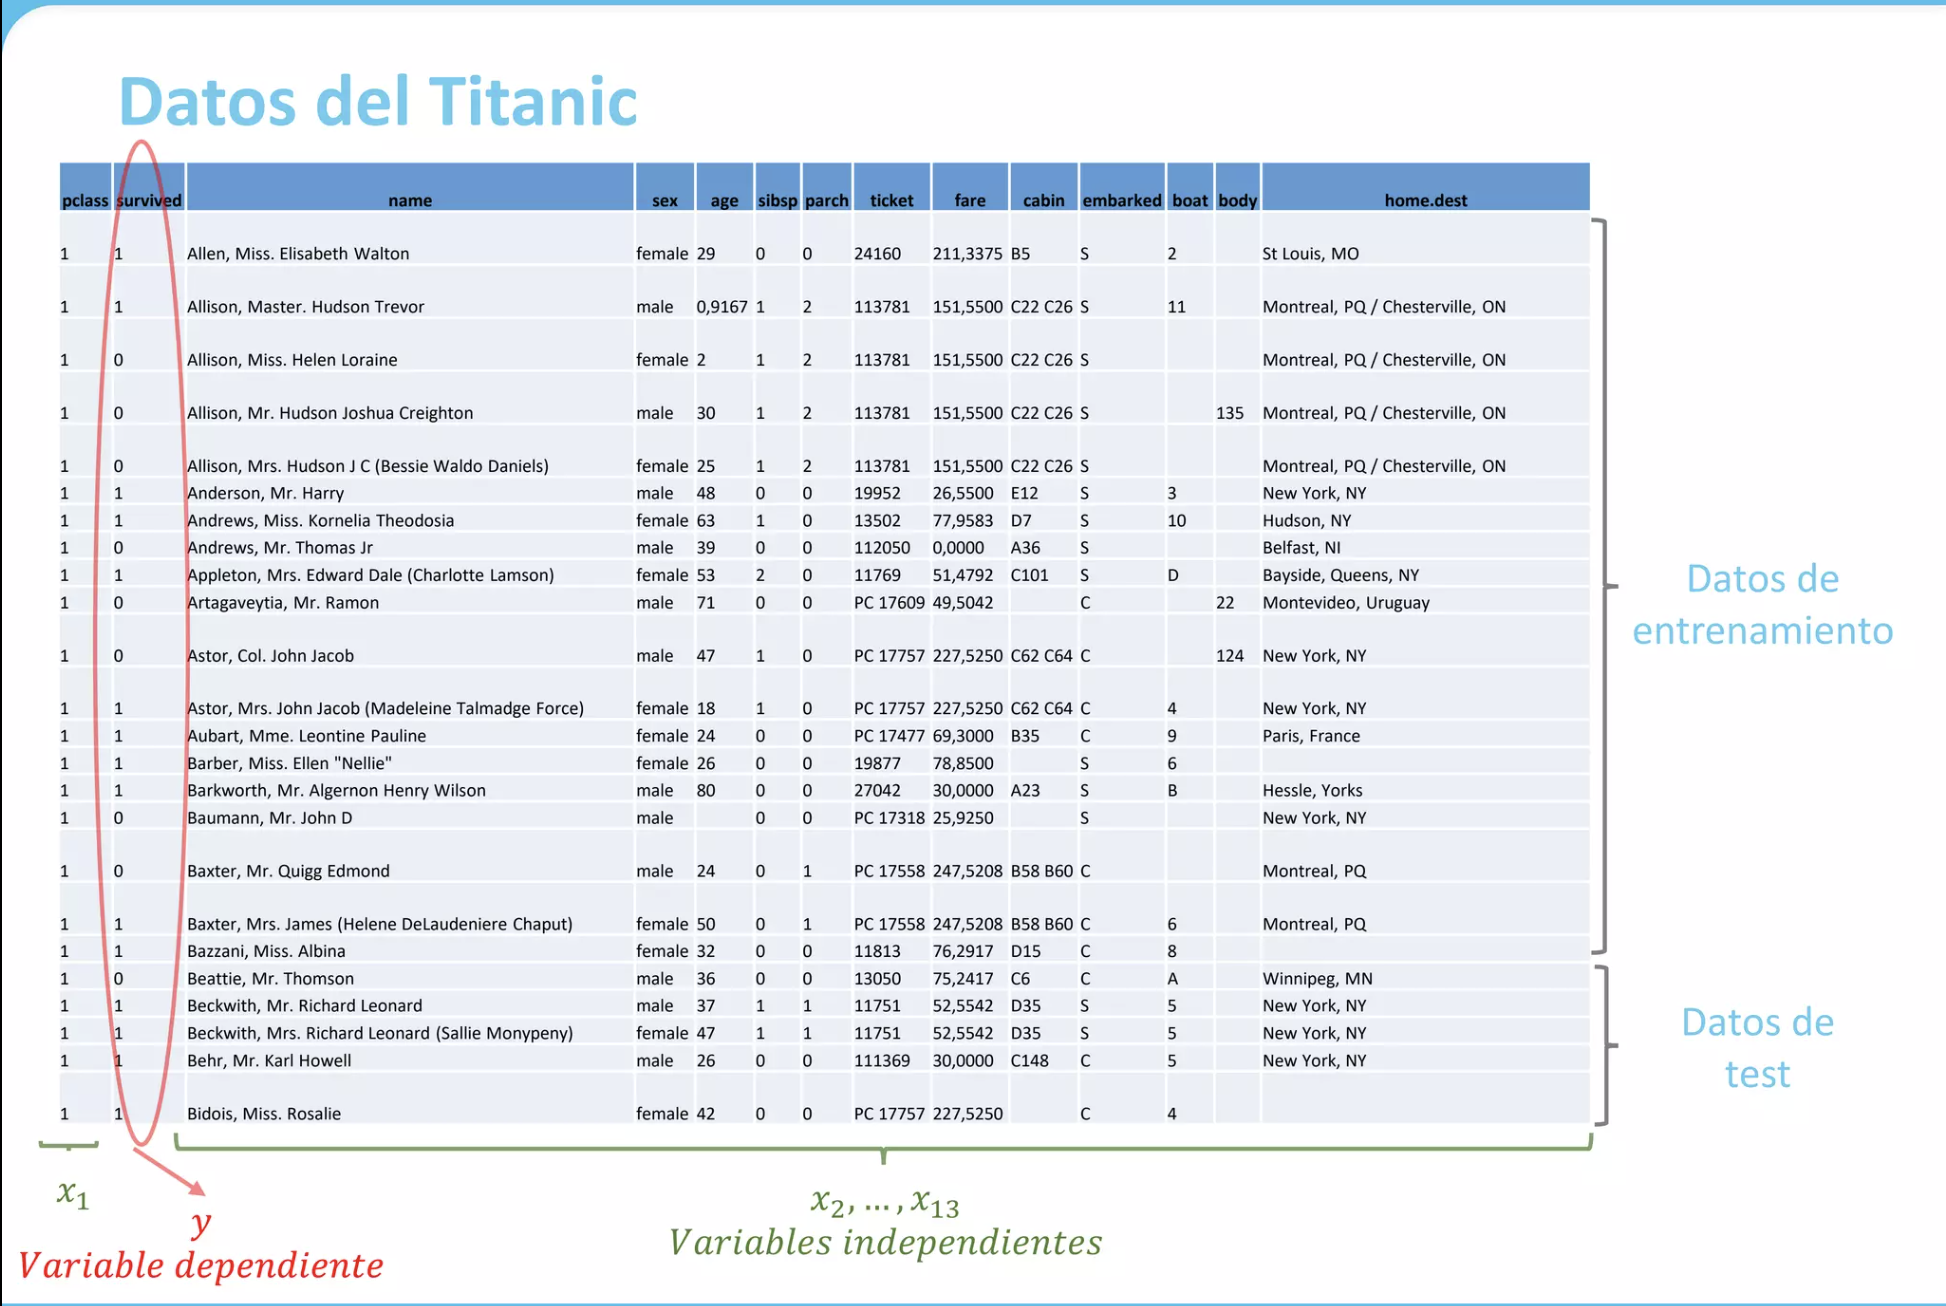
\includegraphics[width=0.7\textwidth]{Titanic}
		\caption{https://es.slideshare.net/JavierEsteveMeli/}
		\centering
	\end{figure}
	\end{block}
\end{frame}


\begin{frame}
	\frametitle{Conceptos en Aprendizaje de Máquina}
		\begin{block}{Categorias}
	
	\begin{itemize}
		\item \textbf{Machine Learning Supervisado}:
		\begin{itemize}
			\item Entrenado con datos que especifican tanto la entrada como la salida.
			\item Por ejemplo, imágenes de números escritos a mano etiquetados con los números correspondientes.
			\item Reconoce patrones y relaciones entre las características y las etiquetas conocidas.
		\end{itemize}
		
		\item \textbf{Machine Learning No Supervisado}:
		\begin{itemize}
			\item Entrenado con datos sin etiquetar.
			\item Analiza datos para encontrar patrones o conexiones significativas.
			\item Agrupa datos en categorías o encuentra estructuras ocultas.
			\item Ejemplo: agrupación de noticias en categorías como deportes o crímenes.
		\end{itemize}
	\end{itemize}
		\end{block}
\end{frame}

\begin{frame}
	\frametitle{Conceptos en Aprendizaje de Máquina}
\begin{block}{Categorías principales del Aprendizaje de Máquina}	
\begin{figure}
	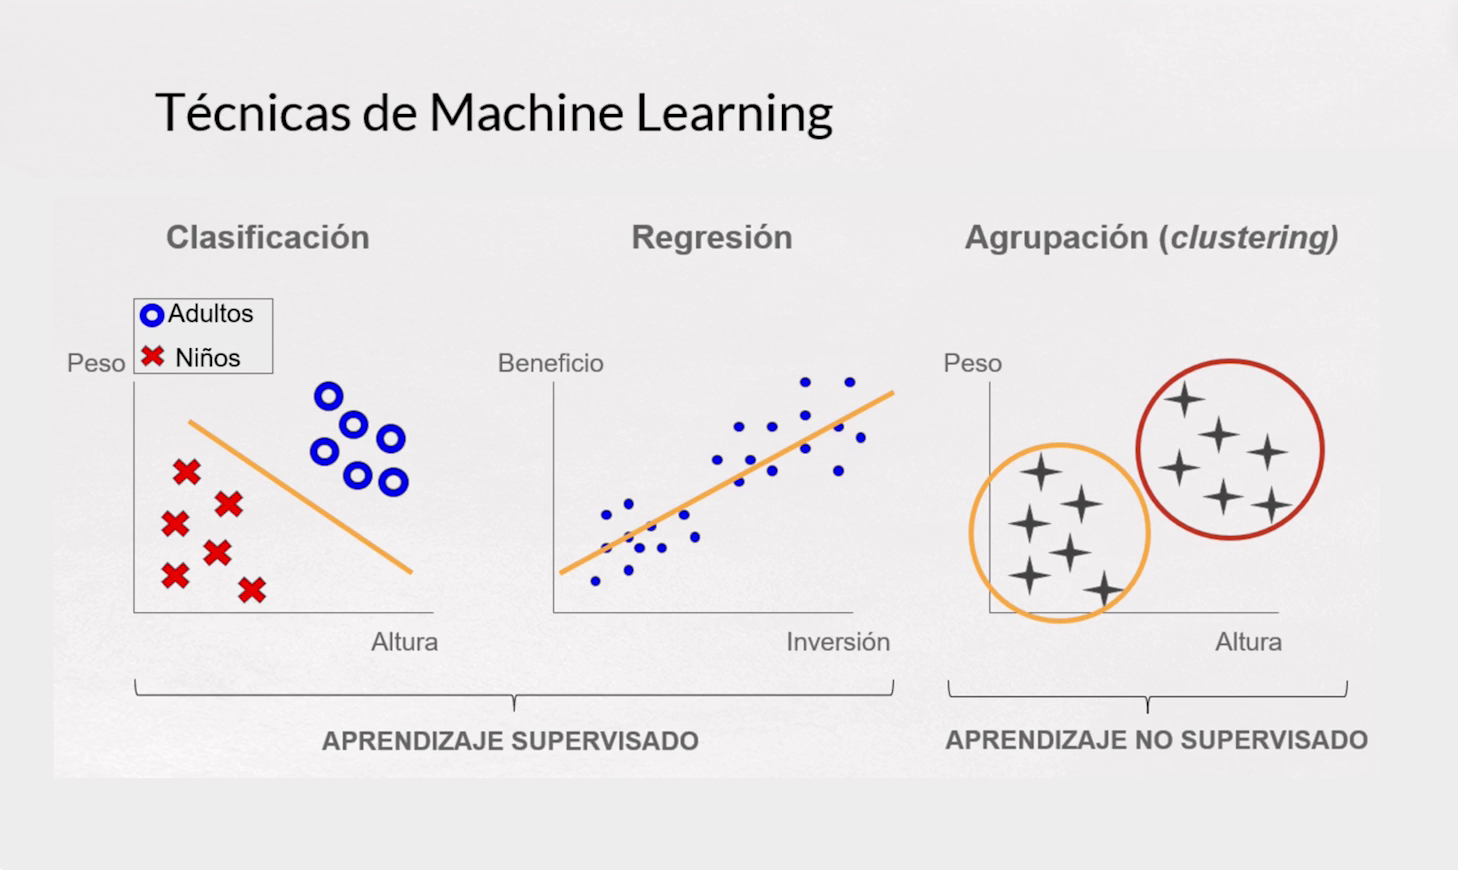
\includegraphics[width=0.9\textwidth]{supervisado_nosupervisado}
	\caption{https://openwebinars.net/blog/modelos-de-machine-learning/}
\end{figure}
\end{block}
\end{frame}



\begin{frame}
	\frametitle{Tipos de Modelos en Aprendizaje de Máquina}
	
	\begin{block}{Modelos Supervisados}
	\begin{itemize}
		\item Regresión lineal
		\item Regresión logística
		\item Máquinas de soporte vectorial (SVM)
		\item Árboles de decisión
		\item Redes neuronales
	\end{itemize}
\end{block}

\end{frame}

	
	\begin{frame}
		\frametitle{Tipos de Modelos en Aprendizaje de Máquina}
			\begin{block}{Modelos No Supervisados}
		\begin{itemize}
			\item K-Means (clustering)
			\item Análisis de Componentes Principales (PCA)
			\item Redes Generativas Adversariales (GANs)
			\item Reglas de asociación
			\item Detección de anomalías
		\end{itemize}
	\end{block}
		\end{frame}
	
	\begin{frame}
		\frametitle{Los Datos en el Aprendizaje de Máquina}
		\begin{block}{Partición de la Data}	
			\begin{figure}
				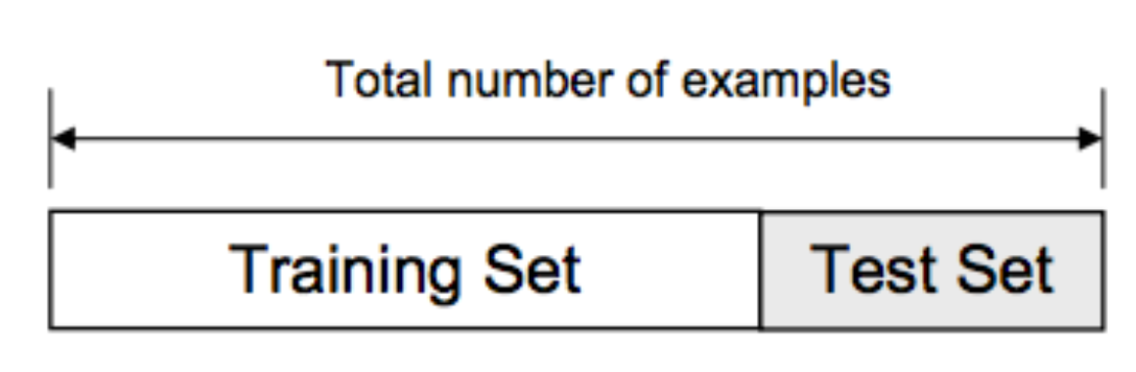
\includegraphics[width=0.7\textwidth]{entrenamiento_prueba}
				\caption{http://exponentis.es/como-dividir-un-conjunto-de-entrenamiento-en-dos-partes-train-test-split}
			\end{figure}
		\end{block}
	\end{frame}
	
	
	
	\begin{frame}
		\frametitle{Partición de la Data}
				\begin{block}{Partición de la Data}	
		\begin{itemize}
		\item  \textbf{Conjunto de Entrenamiento:} 
		Este conjunto se utiliza para entrenar el modelo. Contiene una parte significativa de los datos y es donde el algoritmo de aprendizaje automático "aprende" a partir de las observaciones. El modelo ajusta sus parámetros utilizando este conjunto de datos.
		\item \textbf{ Conjunto de Prueba:} 
		Este conjunto se utiliza para evaluar el rendimiento del modelo una vez que ha sido entrenado. Contiene datos que el modelo no ha visto durante el proceso de entrenamiento. Se utiliza para simular cómo el modelo se comportaría en la práctica al hacer predicciones en datos no vistos.
			\end{itemize}
				\end{block}
\end{frame}

\begin{frame}
	\frametitle{Función de Costo en Modelos}
			\begin{block}{Función de Costo en modelos supervisados}	
	\begin{itemize}
		\item También conocida como función de pérdida o función de error.
		\item Mide qué tan bien se hacen las predicciones del modelo en comparación con los valores reales en el conjunto de entrenamiento.
	\end{itemize}
		\end{block}
\end{frame}

\begin{frame}
	\frametitle{Función de Costo}
	\begin{block}{Función de Costo en Modelos Supervisados}	
		\begin{figure}
	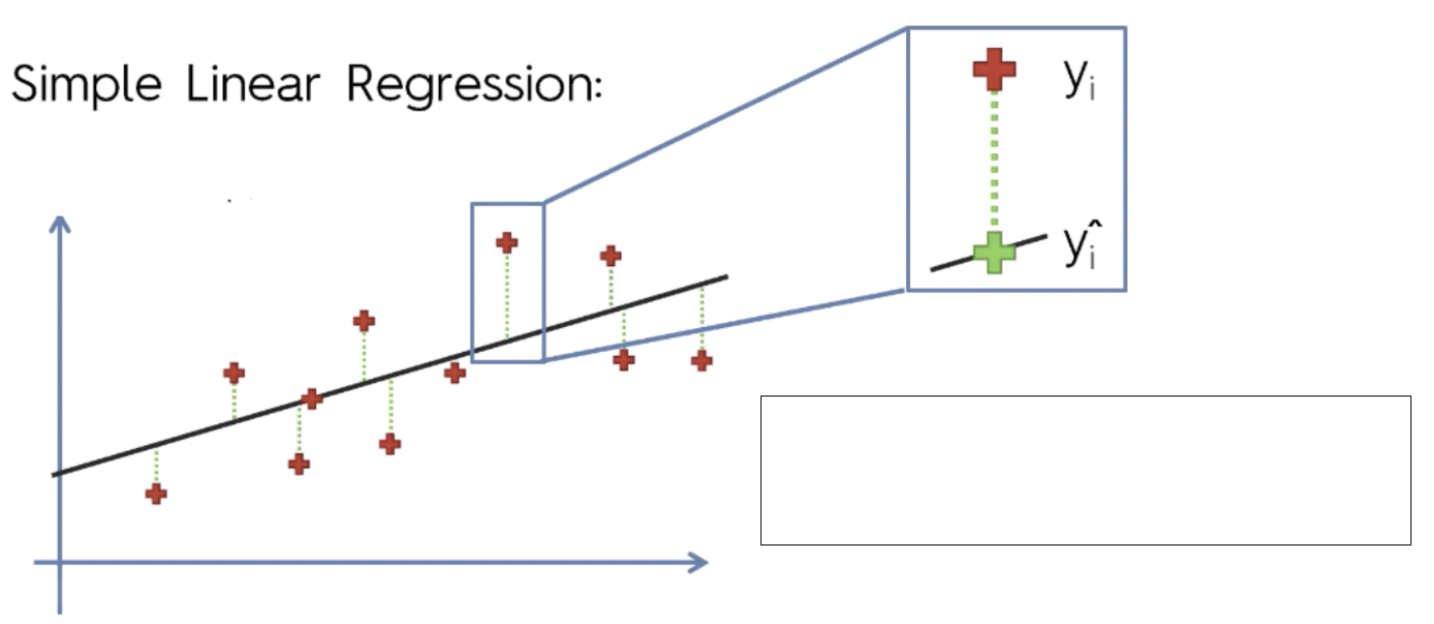
\includegraphics[width=0.9\textwidth]{funcion_coste}
	\caption{https://www.themachinelearners.com/}
\end{figure}
	\end{block}
\end{frame}

\begin{frame}
	\frametitle{Evaluación del Error}
		\begin{block}{Función de Costo en Modelos Supervisados}	
	\begin{itemize}
		\item La función de costo cuantifica la discrepancia entre las predicciones del modelo y los valores reales.
		\item Evalúa la calidad de las predicciones en el conjunto de entrenamiento.
				\item Durante el proceso de entrenamiento, la función de costo se utiliza para ajustar los parámetros del modelo.
		\item El objetivo es encontrar los valores de parámetros que minimizan la función de costo.
	\end{itemize}
		\end{block}
\end{frame}




\begin{frame}
	\frametitle{Funciones de Costo}
			\begin{block}{Función de Costo en Modelos Supervisados}	
				La elección de la función de costo depende del tipo de problema de Machine Learning:
	\begin{itemize}
		\item \textbf{MSE (Mean Squared Error)}: Utilizado en problemas de regresión.
		\item \textbf{Entropía Cruzada (Cross-Entropy)}: Utilizado en problemas de clasificación.
	\end{itemize}
	\end{block}
\end{frame}

\begin{frame}
	\frametitle{Función de Costo}
			\begin{block}{Función de Costo en Modelos No Supervisados}	
	\begin{itemize}
		\item En modelos no supervisados, también se utilizan funciones de costo.
		\item Estas funciones miden la calidad de las soluciones o guían el proceso de aprendizaje no supervisado.
	\end{itemize}
		\end{block}
\end{frame}

\begin{frame}
	\frametitle{Función de Costo}
		\begin{block}{Función de Costo en Modelos No Supervisados}	
	\begin{itemize}
		\item En K-Medias (Clustering), se utiliza la función de costo \textbf{``inercia"} o \textbf{``SSE"} para minimizar la distancia de las instancias a los centroides.
			\item Aunque \textbf{PCA} no se ajusta en el sentido tradicional, busca una solución que\textbf{ optimice la varianza }de las proyecciones de datos.
	\end{itemize}
	\end{block}
\end{frame}

\section{MODELOS DE REGRESIÓN}

\begin{frame}
			\frametitle{MODELOS DE APRENDIZAJE DE MÁQUINA}
	\begin{block}{}	
		\center
		\textbf{MODELOS DE REGRESIÓN}
	\end{block}
\end{frame}


\begin{frame}
	\frametitle{MODELOS DE REGRESIÓN}
\begin{block}{Regresión}	
		\begin{figure}
			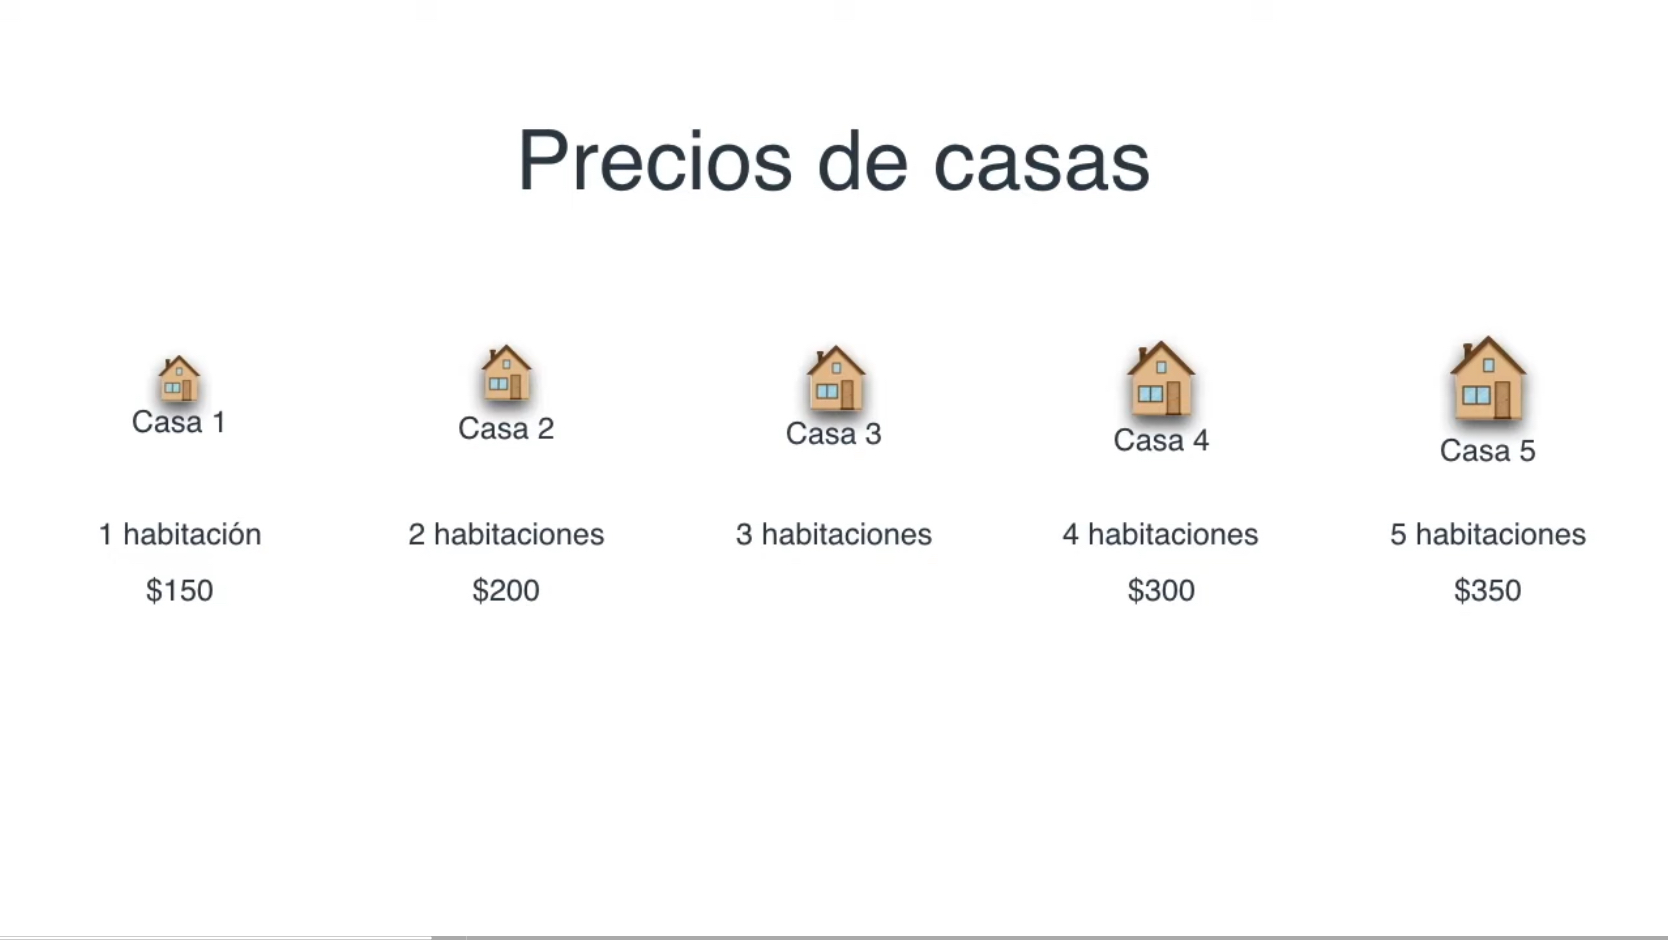
\includegraphics[width=0.9\textwidth]{imagenes_regresion/IMG_3483.jpg}
			\caption{https://serrano.academy/espanol/}
		\end{figure}
	\end{block}
\end{frame}

\begin{frame}
	\frametitle{MODELOS DE REGRESIÓN}
	\begin{block}{Regresión}	
		\begin{figure}
			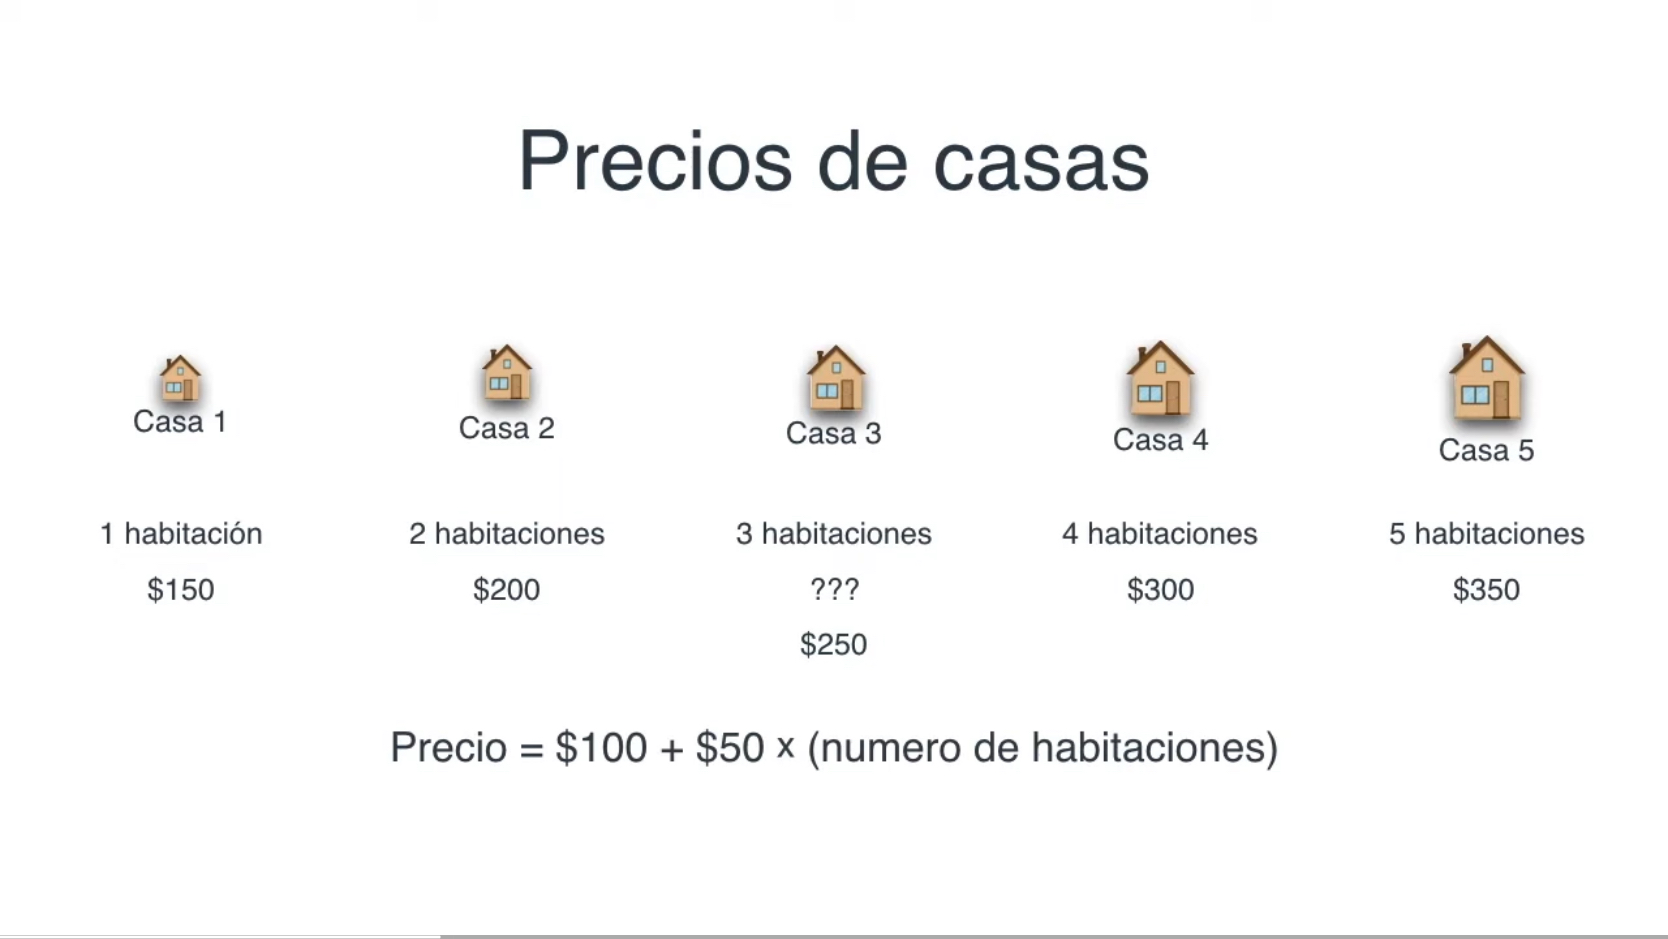
\includegraphics[width=0.9\textwidth]{imagenes_regresion/IMG_3483_1.jpeg}
			\caption{https://serrano.academy/espanol/}
		\end{figure}
	\end{block}
\end{frame}

\begin{frame}
	\frametitle{MODELOS DE REGRESIÓN}
\begin{block}{Regresión}	
		\begin{figure}
			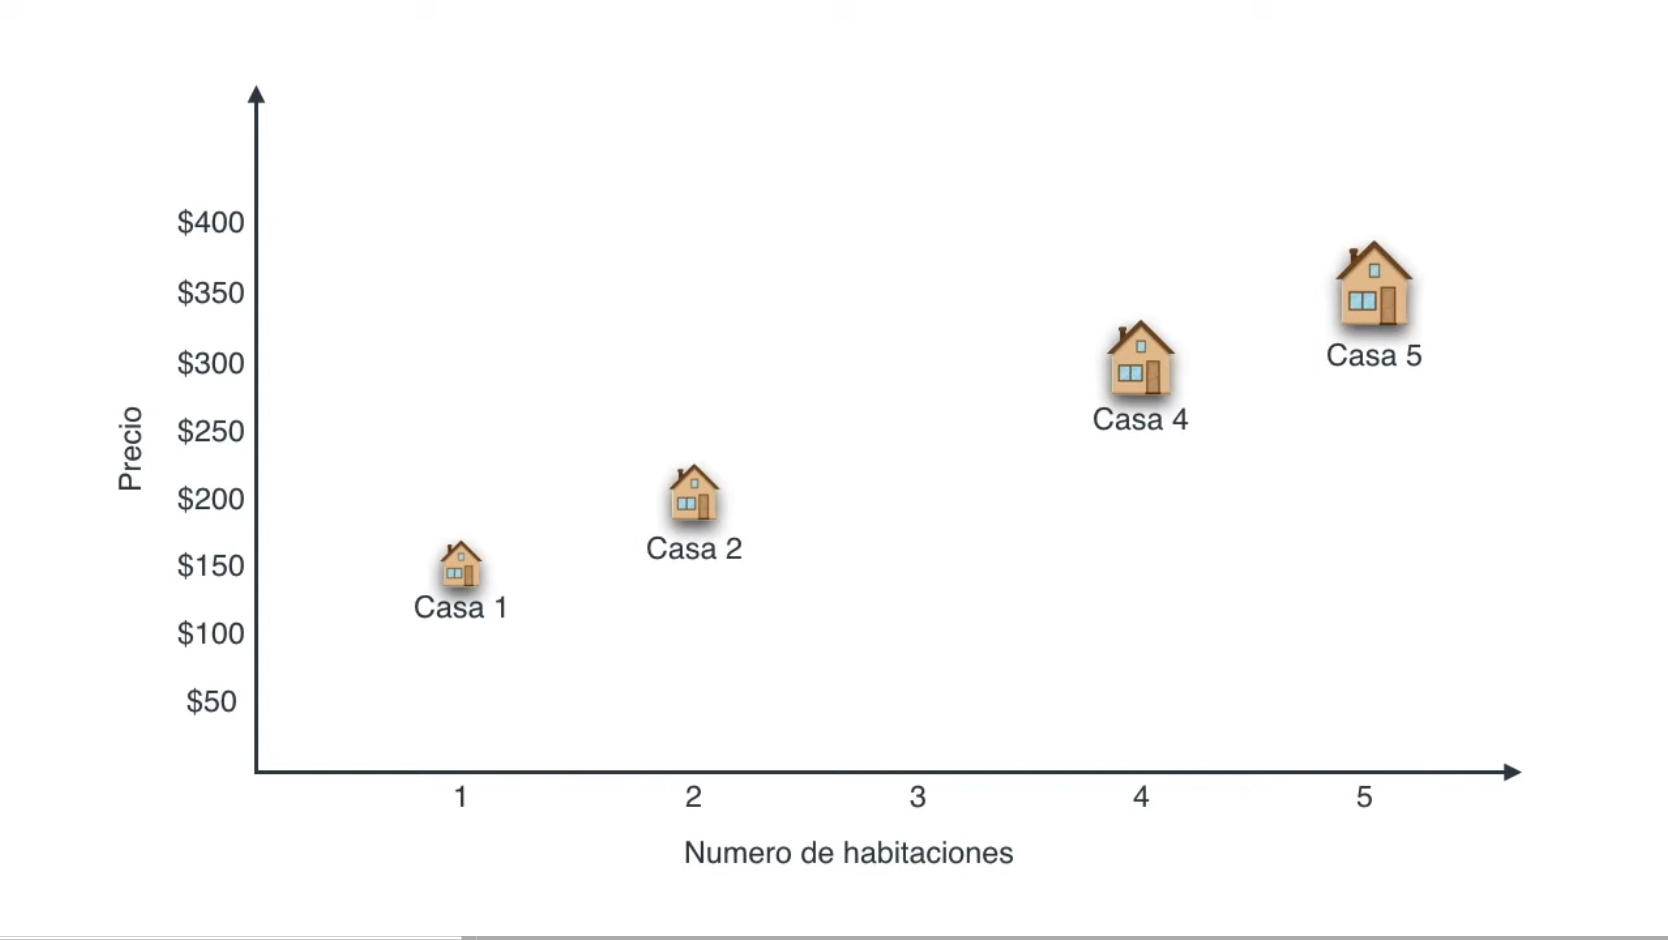
\includegraphics[width=0.9\textwidth]{imagenes_regresion/IMG_3484.jpg}
			\caption{https://serrano.academy/espanol/}
		\end{figure}
	\end{block}
\end{frame}

\begin{frame}
	\frametitle{MODELOS DE REGRESIÓN}
	\begin{block}{Regresión}	
		\begin{figure}
			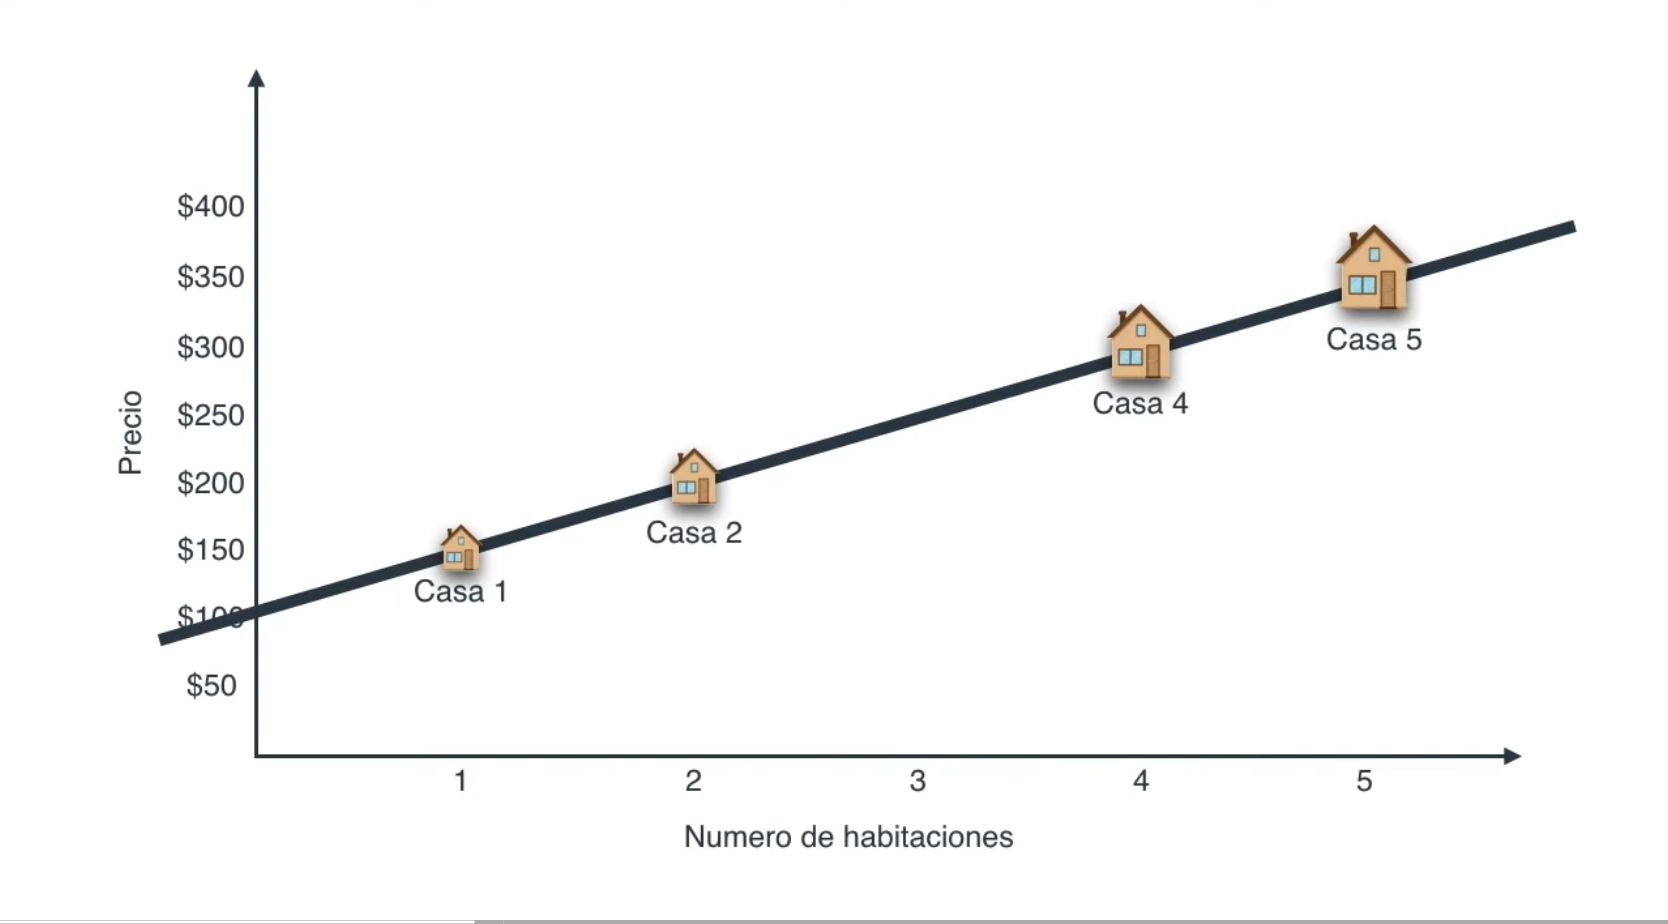
\includegraphics[width=0.9\textwidth]{imagenes_regresion/IMG_3485.jpg}
		\caption{https://serrano.academy/espanol/}
		\end{figure}
	\end{block}
\end{frame}

\begin{frame}
	\frametitle{MODELOS DE REGRESIÓN}
\begin{block}{Regresión}	
		\begin{figure}
			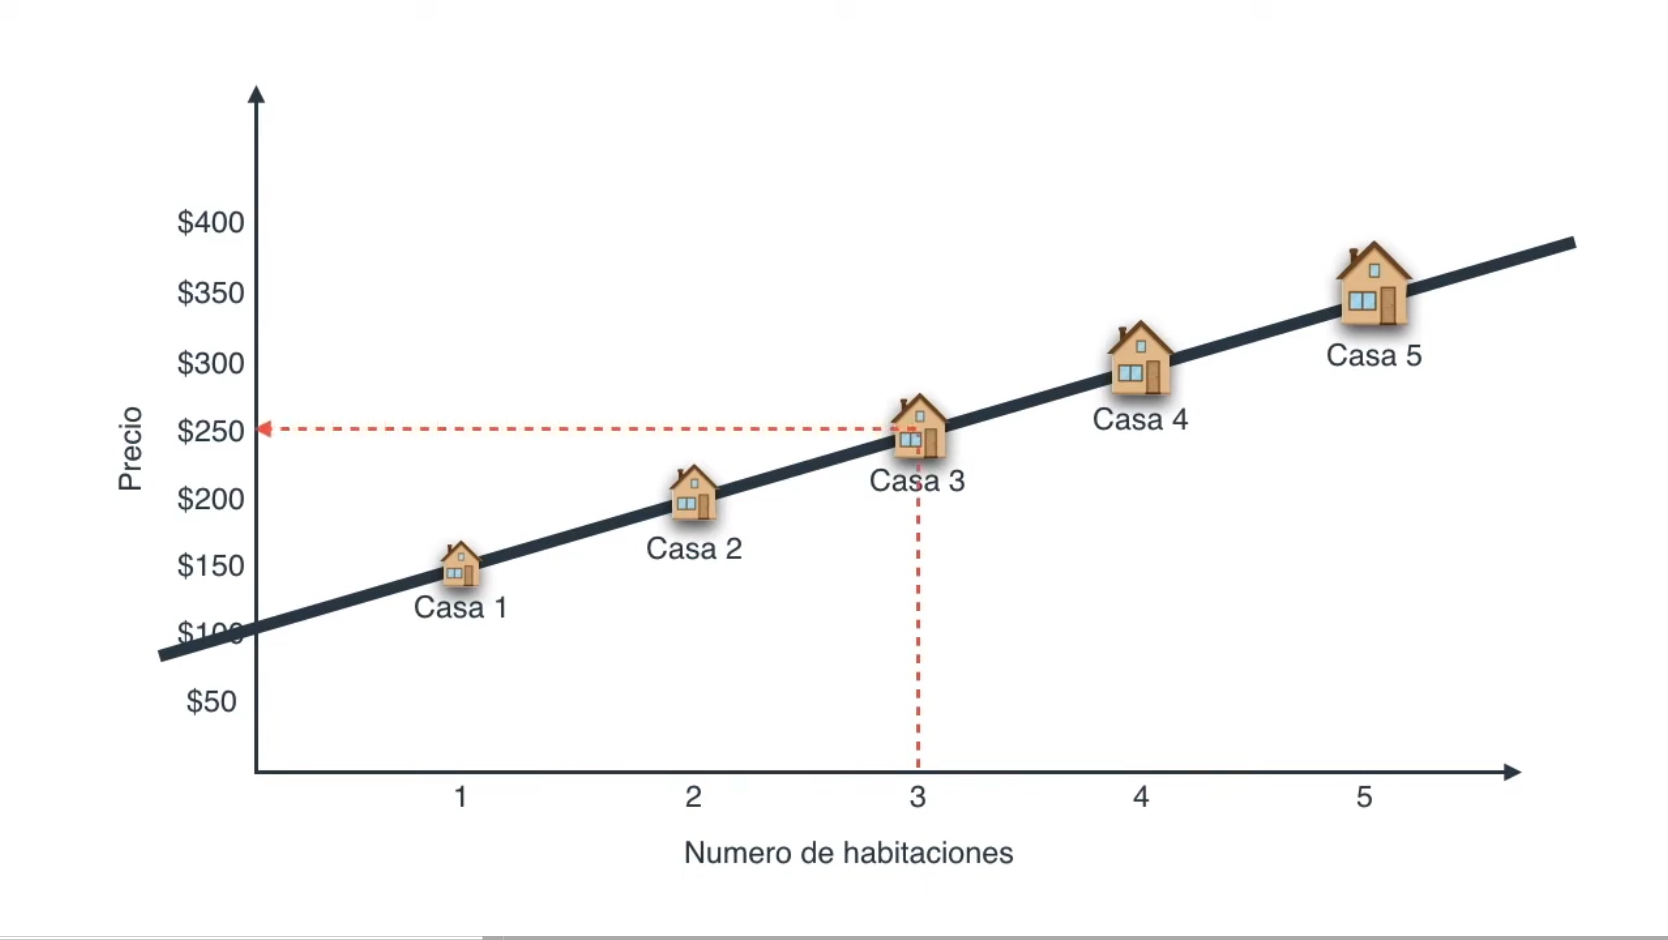
\includegraphics[width=0.9\textwidth]{imagenes_regresion/IMG_3486.jpg}
			\caption{https://serrano.academy/espanol/}
		\end{figure}
	\end{block}
\end{frame}

\begin{frame}
	\frametitle{MODELOS DE REGRESIÓN}
\begin{block}{Regresión}	
		\begin{figure}
			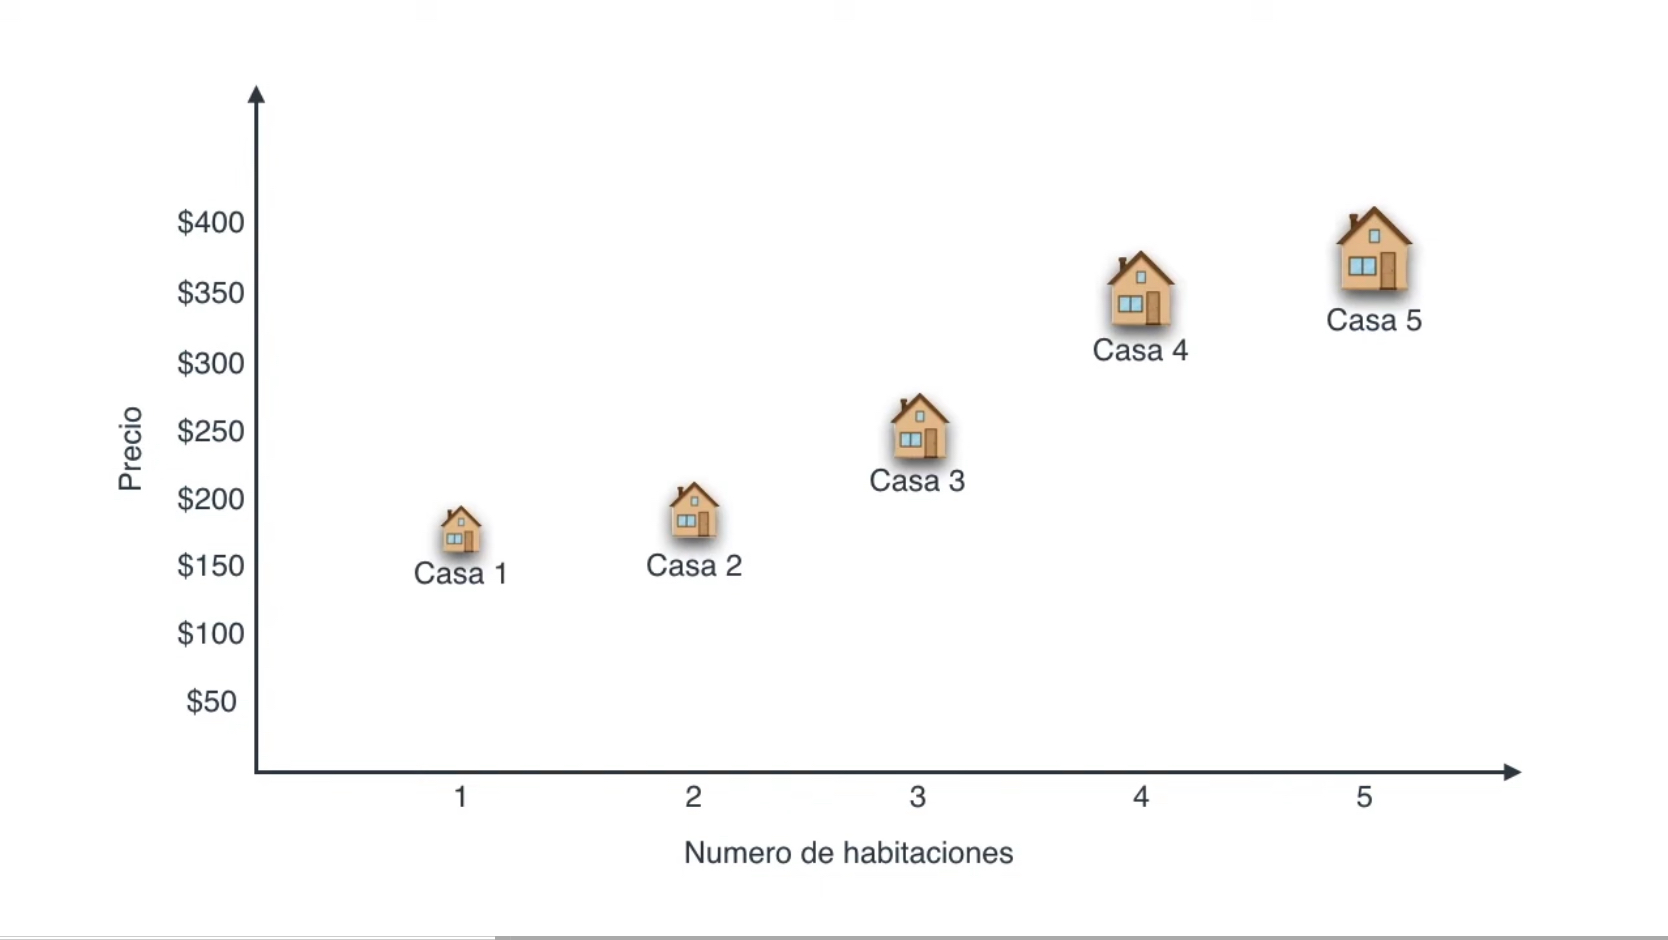
\includegraphics[width=0.9\textwidth]{imagenes_regresion/IMG_3487.jpg}
			\caption{https://serrano.academy/espanol/}
		\end{figure}
	\end{block}
\end{frame}

\begin{frame}
	\frametitle{MODELOS DE REGRESIÓN}
\begin{block}{Regresión}	
		\begin{figure}
			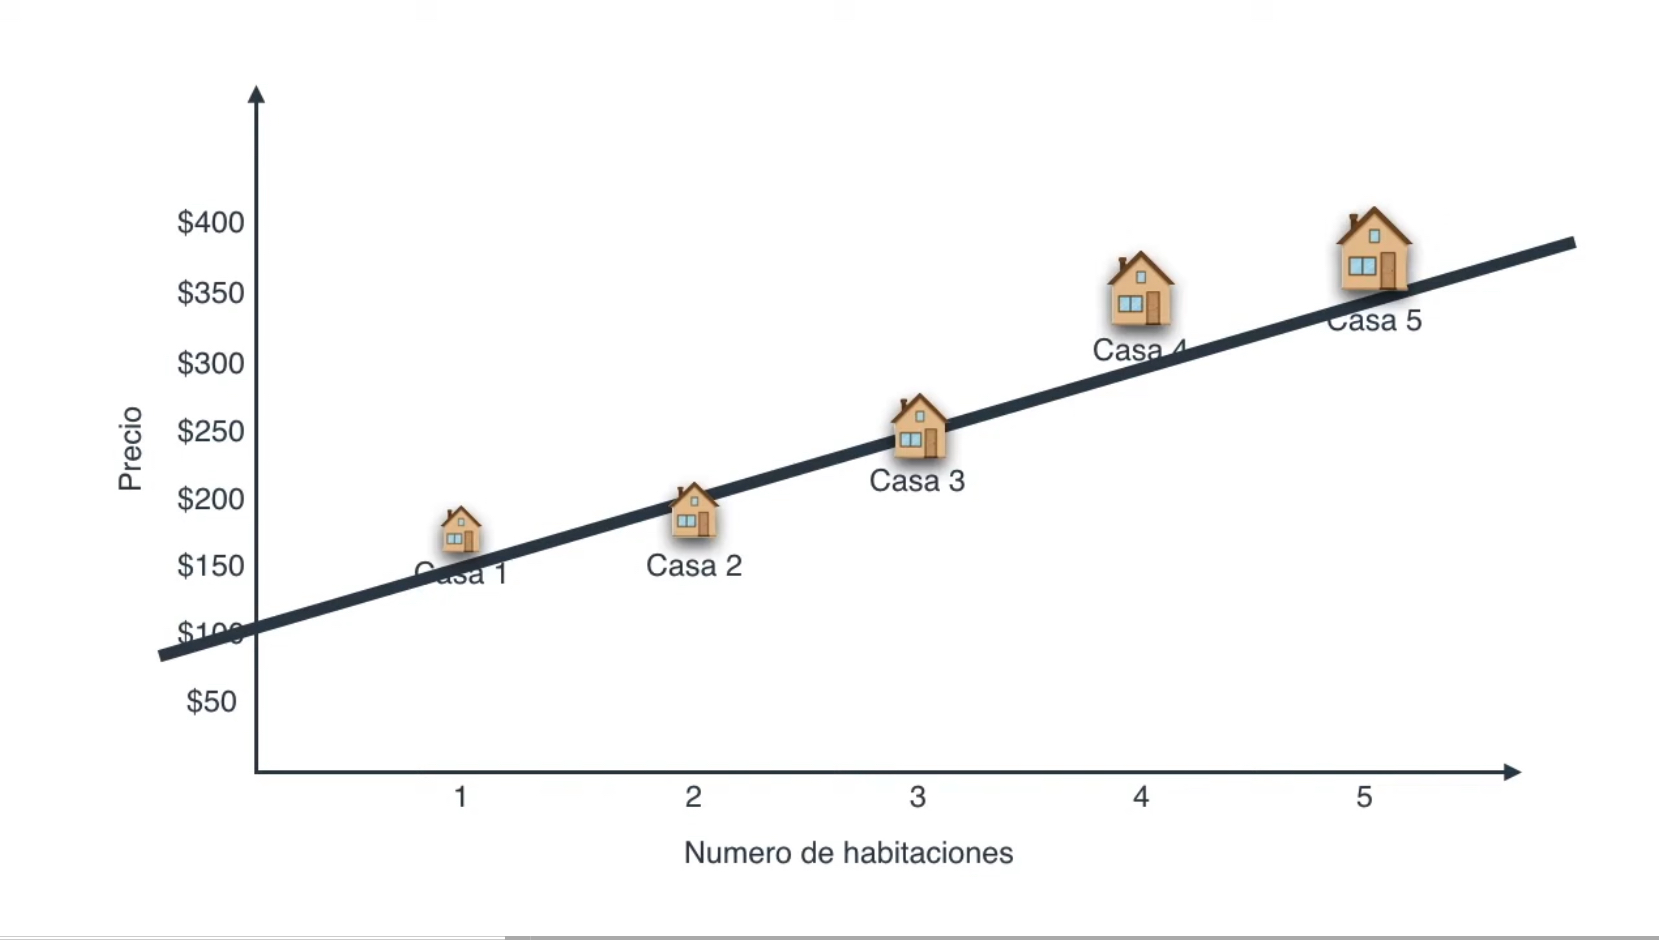
\includegraphics[width=0.9\textwidth]{imagenes_regresion/IMG_3488.jpg}
			\caption{https://serrano.academy/espanol/}
		\end{figure}
	\end{block}
\end{frame}

\begin{frame}
	\frametitle{MODELOS DE REGRESIÓN}
\begin{block}{Regresión}	
		\begin{figure}
			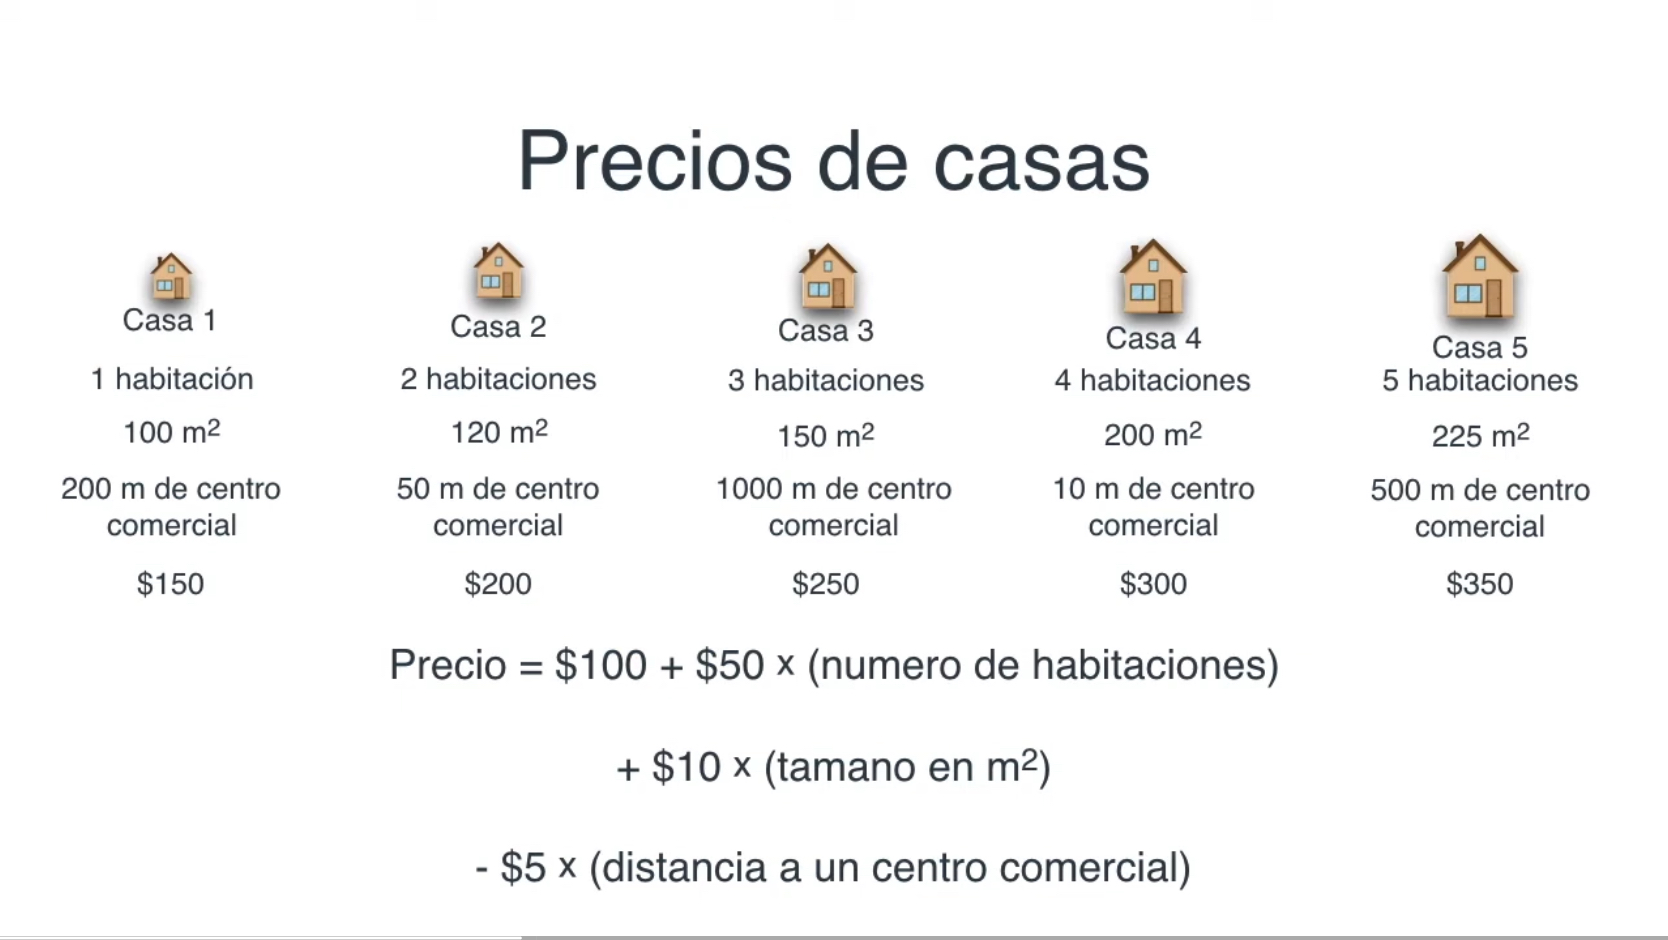
\includegraphics[width=0.9\textwidth]{imagenes_regresion/IMG_3489.jpg}
			\caption{https://serrano.academy/espanol/}
		\end{figure}
	\end{block}
\end{frame}


\section{MODELOS DE REGRESIÓN LOGÍSTICA}

\begin{frame}
		\frametitle{MODELOS DE APRENDIZAJE DE MÁQUINA}
	\begin{block}{}	
		\center
		\textbf{MODELOS DE REGRESIÓN LOGÍSTICA}
	\end{block}
\end{frame}

\begin{frame}
	\frametitle{MODELOS DE REGRESIÓN}
	\begin{block}{Regresión Logística}	
		\begin{figure}
			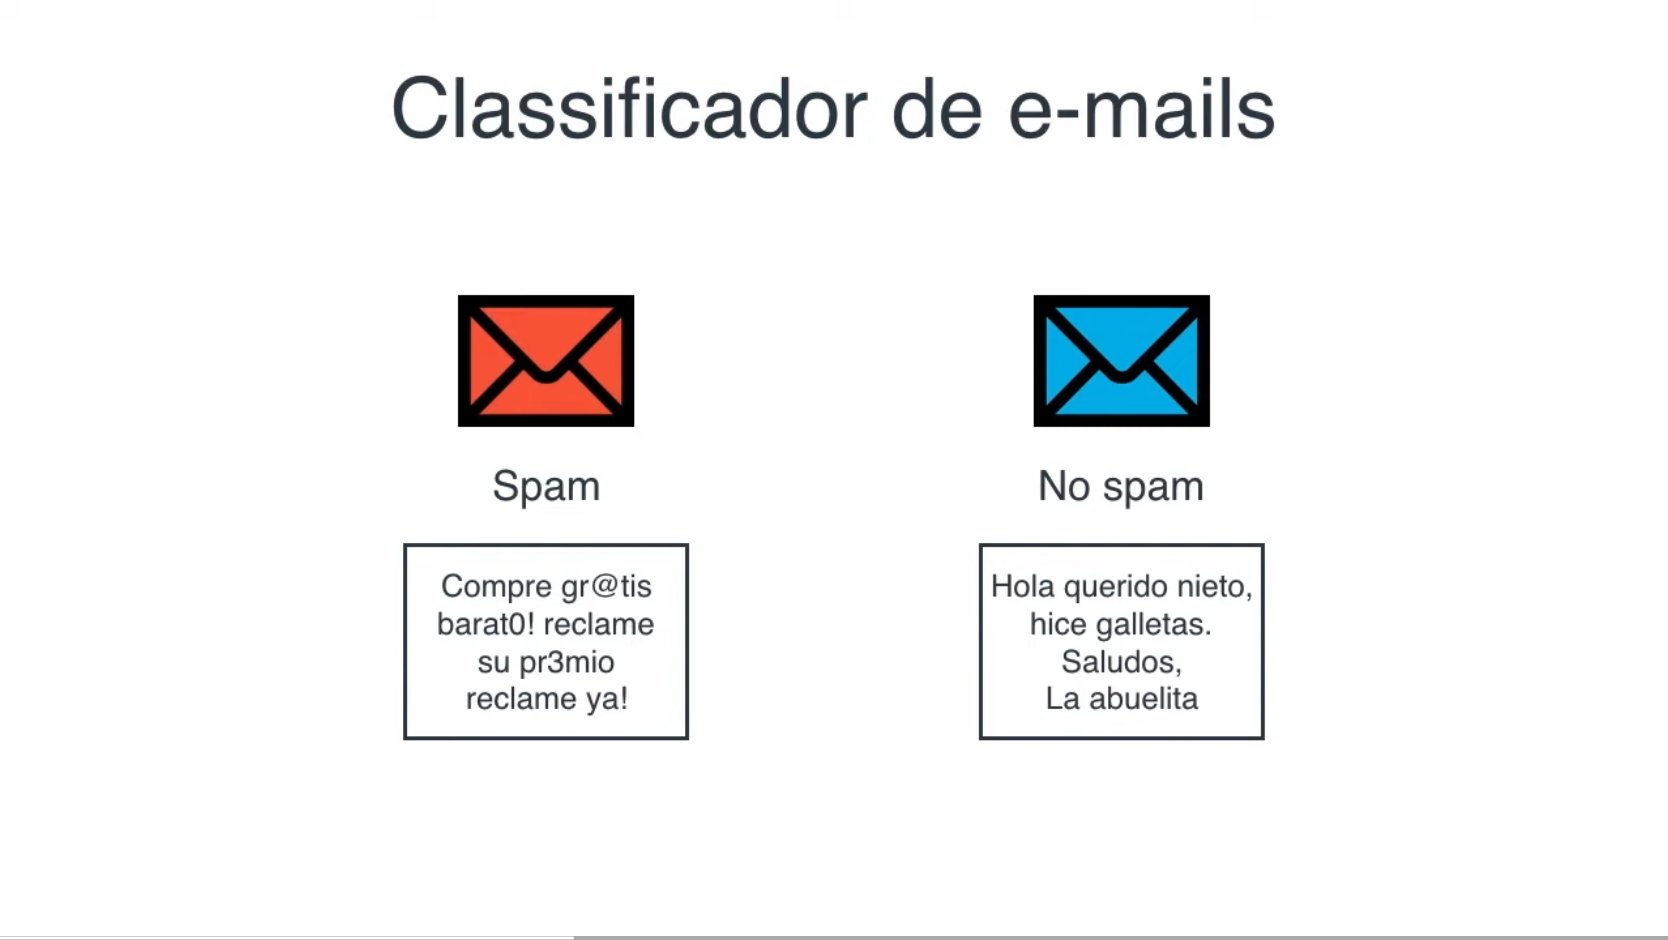
\includegraphics[width=0.9\textwidth]{Imagenes_reg_log/IMG_3490.jpg}
			\caption{https://serrano.academy/espanol/}
		\end{figure}
	\end{block}
\end{frame}

\begin{frame}
	\frametitle{MODELOS DE REGRESIÓN}
	\begin{block}{Regresión Logística}	
		\begin{itemize}
			\item \textbf{Candidata 1}: Si tiene la palabra \textit{``reclame"}, entonces es spam. De lo contrario, no.
			\item \textbf{Candidata 2}: Si tiene dos errores de ortografía, entonces es spam. De lo contrario, no.
			\item \textbf{Candidata 3}: Si tiene la palabra \textit{``reclame"} dos veces, y tres errores de ortografía, entonces es spam. De lo contrario, no.
			\item \textbf{Candidata 4}: Si el número de veces que aparece la palabra \textit{``reclame"} más el número de errores de ortografía es mayor a 4, entonces es spam. De lo contrario, no.
		\end{itemize}
		%\begin{figure}
		%	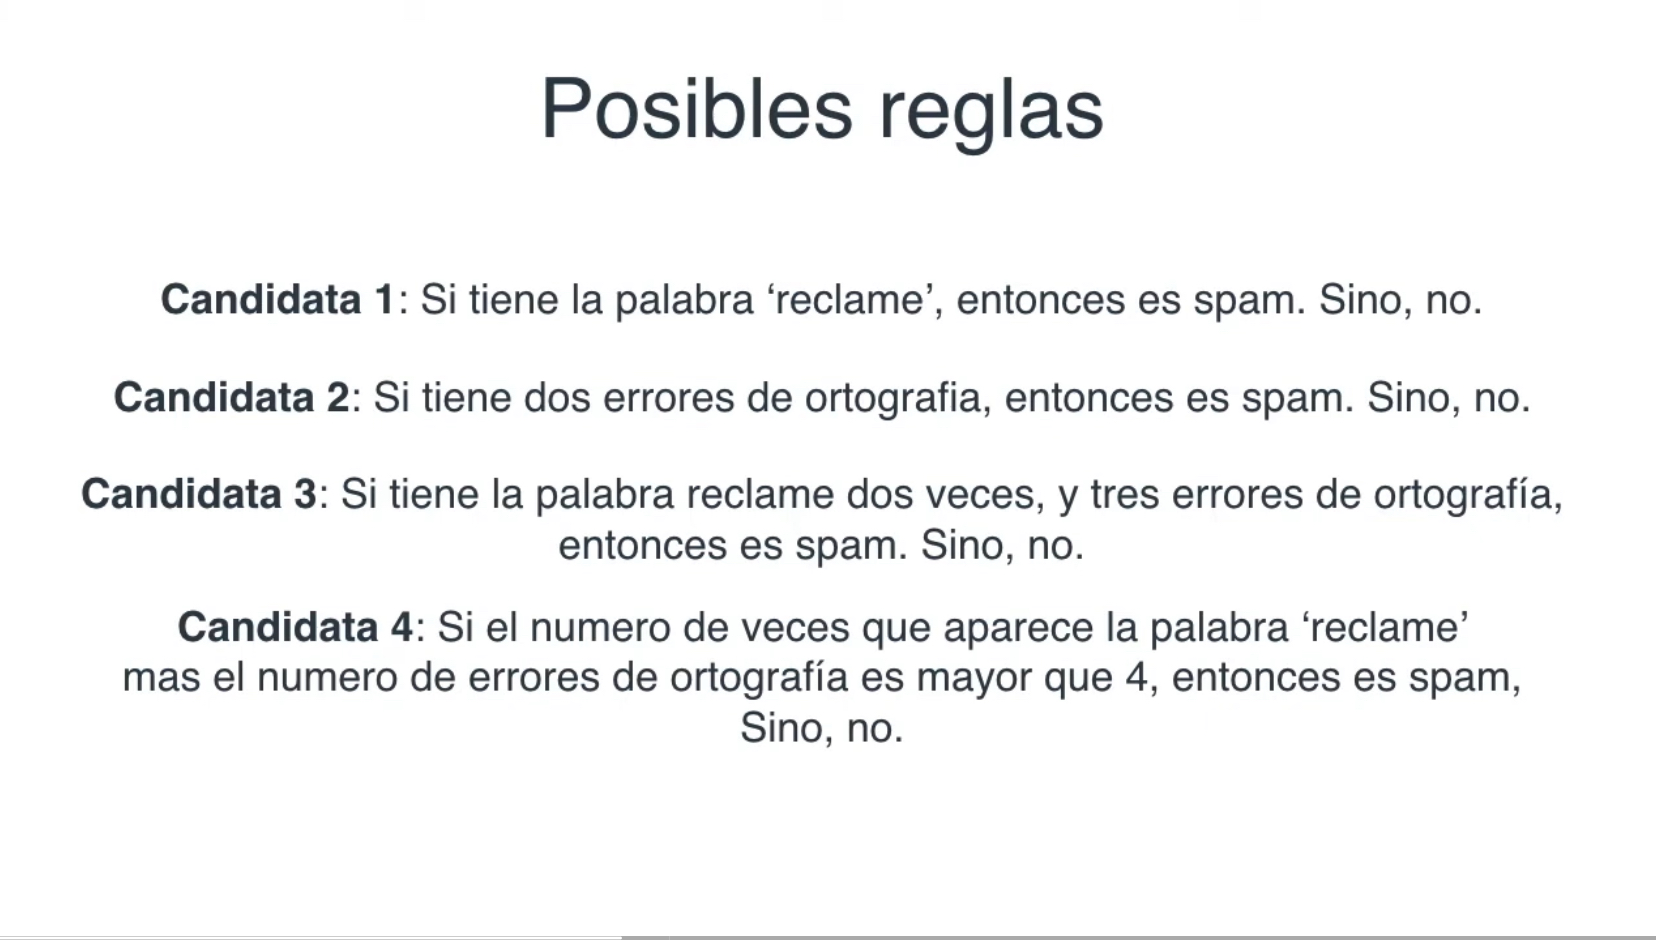
\includegraphics[width=0.9\textwidth]{Imagenes_reg_log/IMG_3491.jpg}
		 %	\caption{https://serrano.academy/espanol/}
		%\end{figure}
	\end{block}
\end{frame}

\begin{frame}
	\frametitle{MODELOS DE REGRESIÓN}
	\begin{block}{Regresión Logística}	
		\begin{figure}
			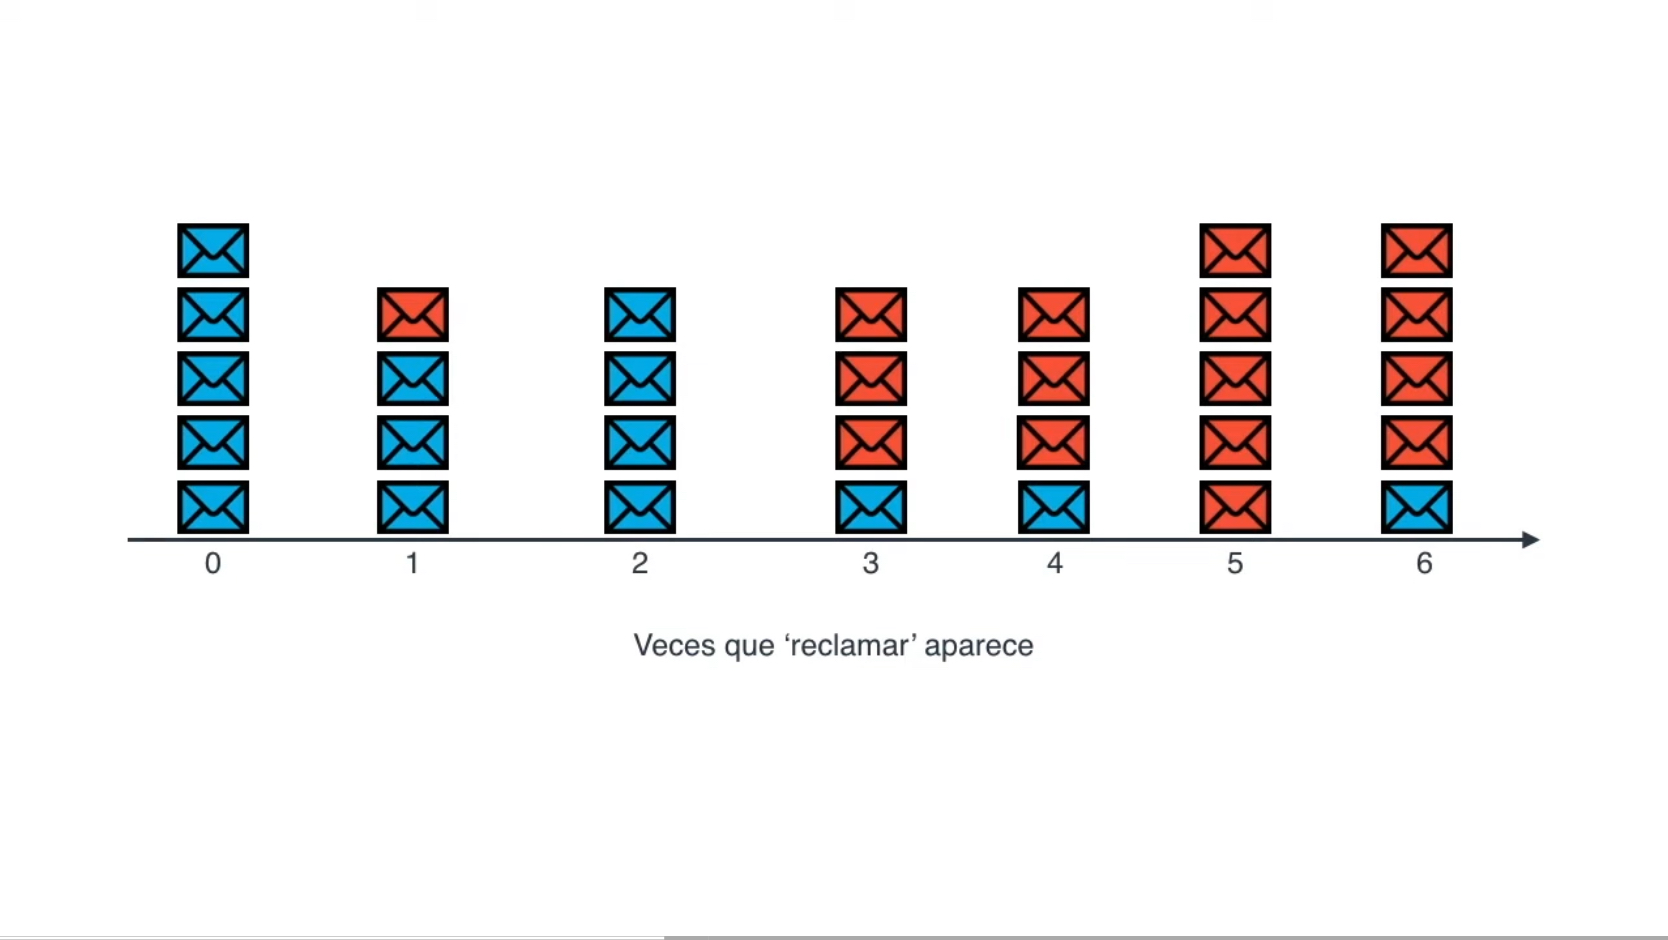
\includegraphics[width=0.9\textwidth]{Imagenes_reg_log/IMG_3492.jpg}
			\caption{https://serrano.academy/espanol/}
		\end{figure}
	\end{block}
\end{frame}

\begin{frame}
	\frametitle{MODELOS DE REGRESIÓN}
	\begin{block}{Regresión Logística}	
		\begin{figure}
			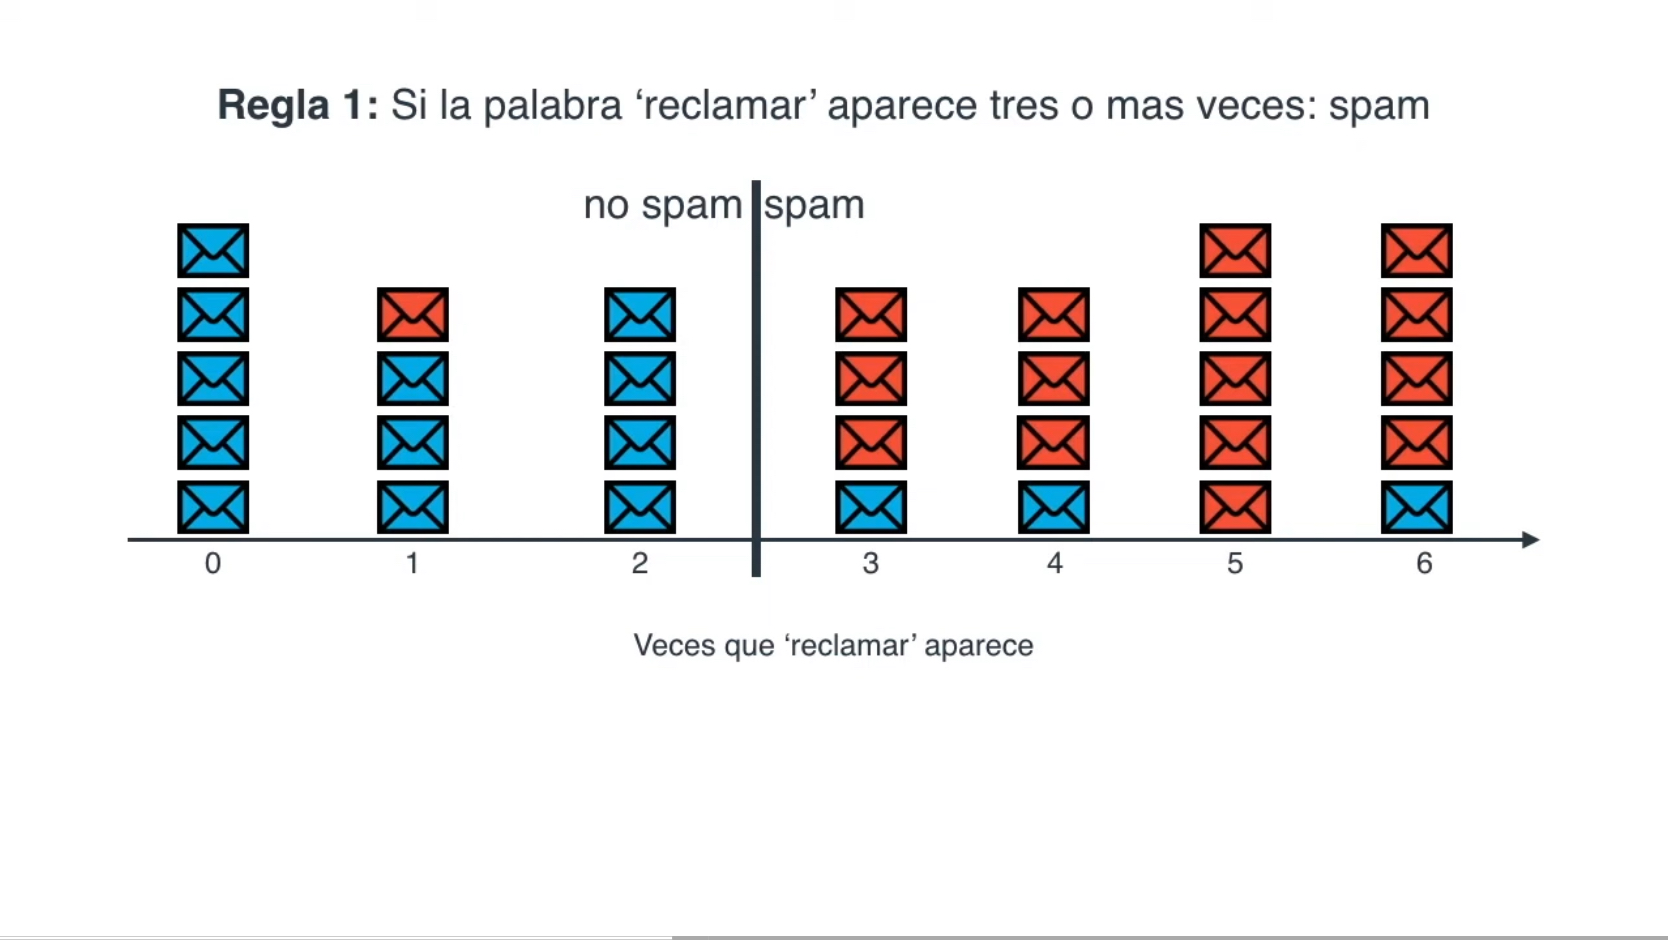
\includegraphics[width=0.9\textwidth]{Imagenes_reg_log/IMG_3493.jpg}
			\caption{https://serrano.academy/espanol/}
		\end{figure}
	\end{block}
\end{frame}

\begin{frame}
	\frametitle{MODELOS DE REGRESIÓN}
	\begin{block}{Regresión Logística}	
		\begin{figure}
			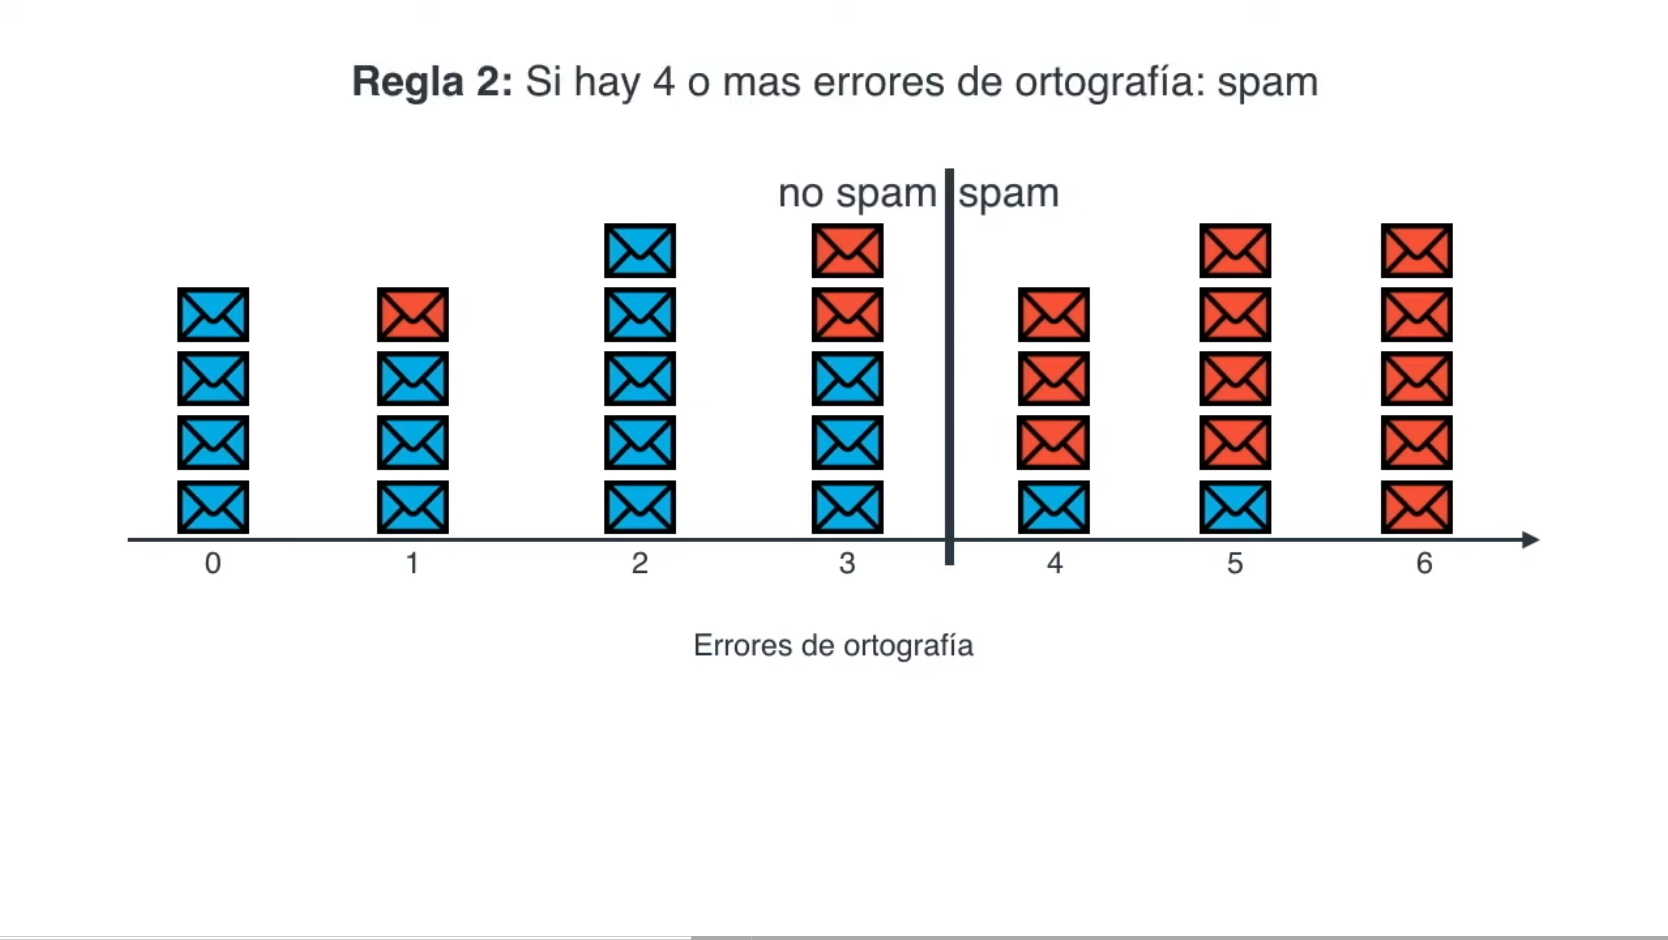
\includegraphics[width=0.9\textwidth]{Imagenes_reg_log/IMG_3496.jpg}
			\caption{https://serrano.academy/espanol/}
		\end{figure}
	\end{block}
\end{frame}


\begin{frame}
	\frametitle{MODELOS DE REGRESIÓN}
	\begin{block}{Regresión Logística}	
		\begin{figure}
			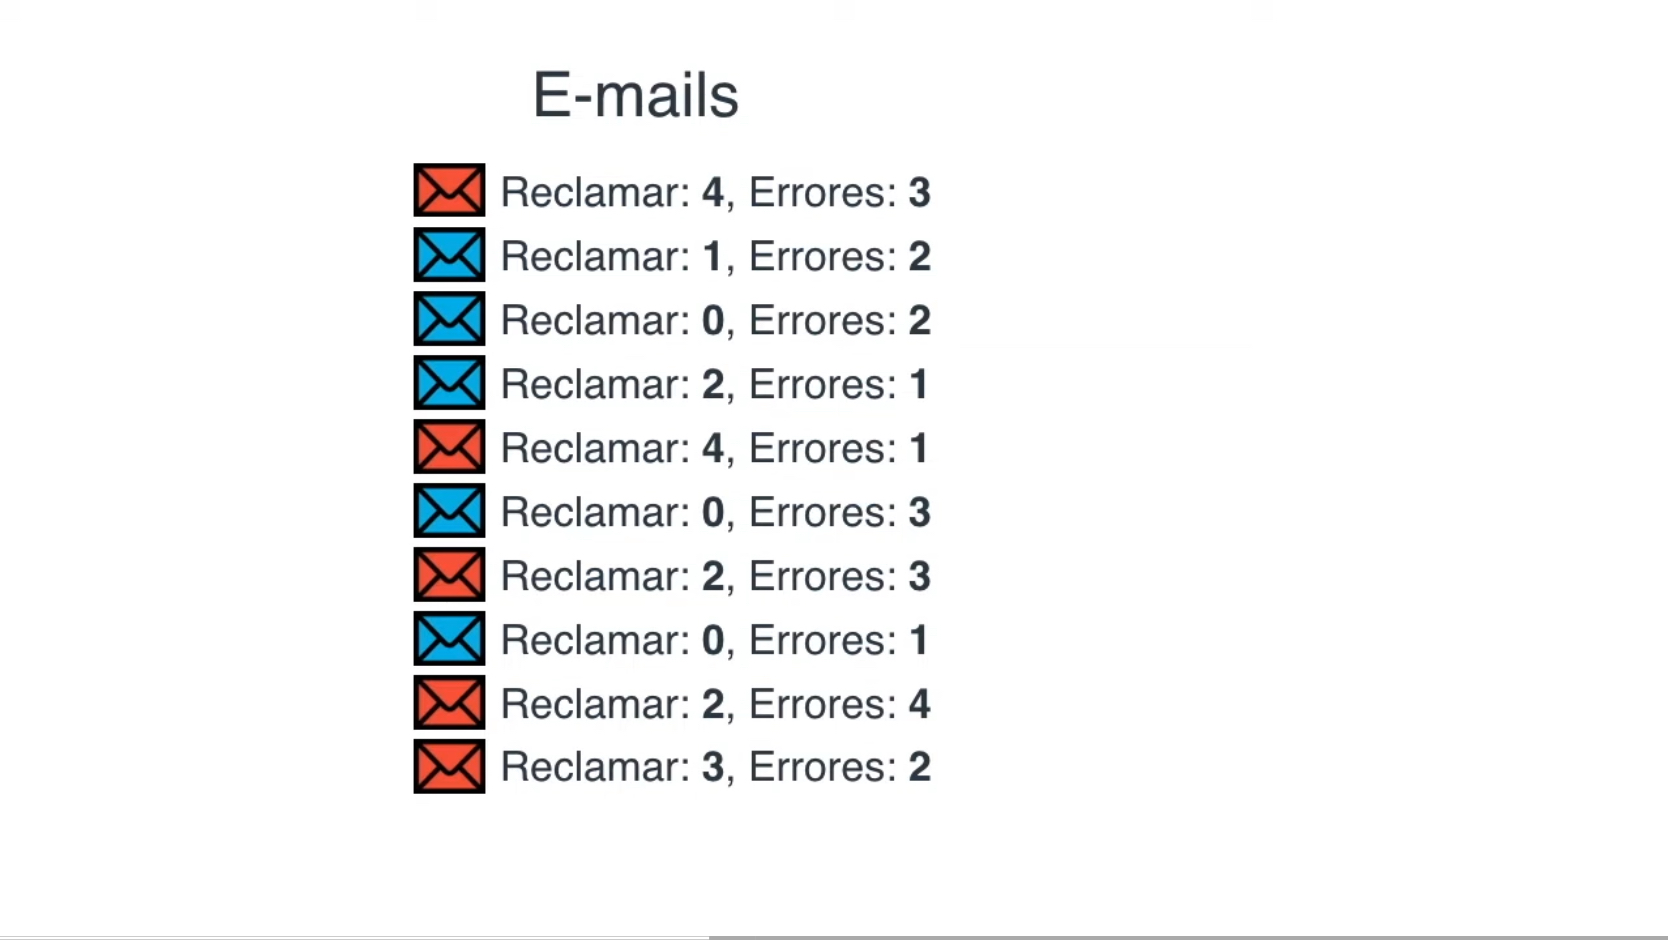
\includegraphics[width=0.9\textwidth]{Imagenes_reg_log/IMG_3497.jpg}
			\caption{https://serrano.academy/espanol/}
		\end{figure}
	\end{block}
\end{frame}
	
\begin{frame}
	\frametitle{MODELOS DE REGRESIÓN}
	\begin{block}{Regresión Logística}	
		\begin{figure}
			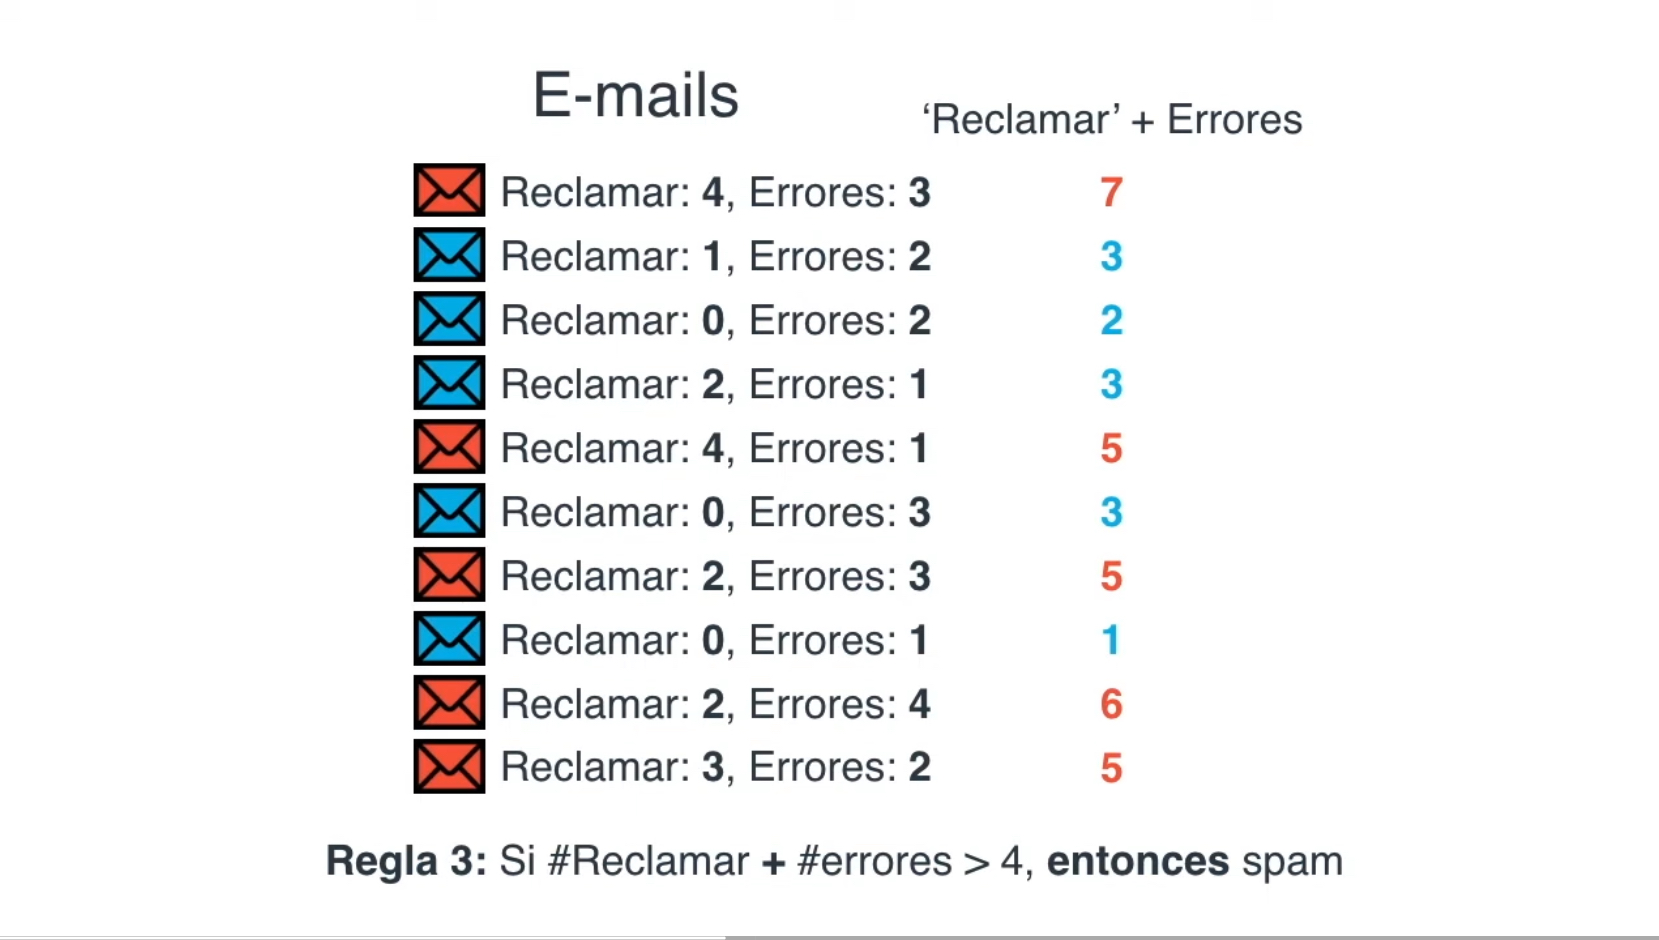
\includegraphics[width=0.9\textwidth]{Imagenes_reg_log/IMG_3498.jpg}
			\caption{https://serrano.academy/espanol/}
		\end{figure}
	\end{block}
\end{frame}

\begin{frame}
	\frametitle{MODELOS DE REGRESIÓN}
	\begin{block}{Regresión Logística}	
		\begin{figure}
			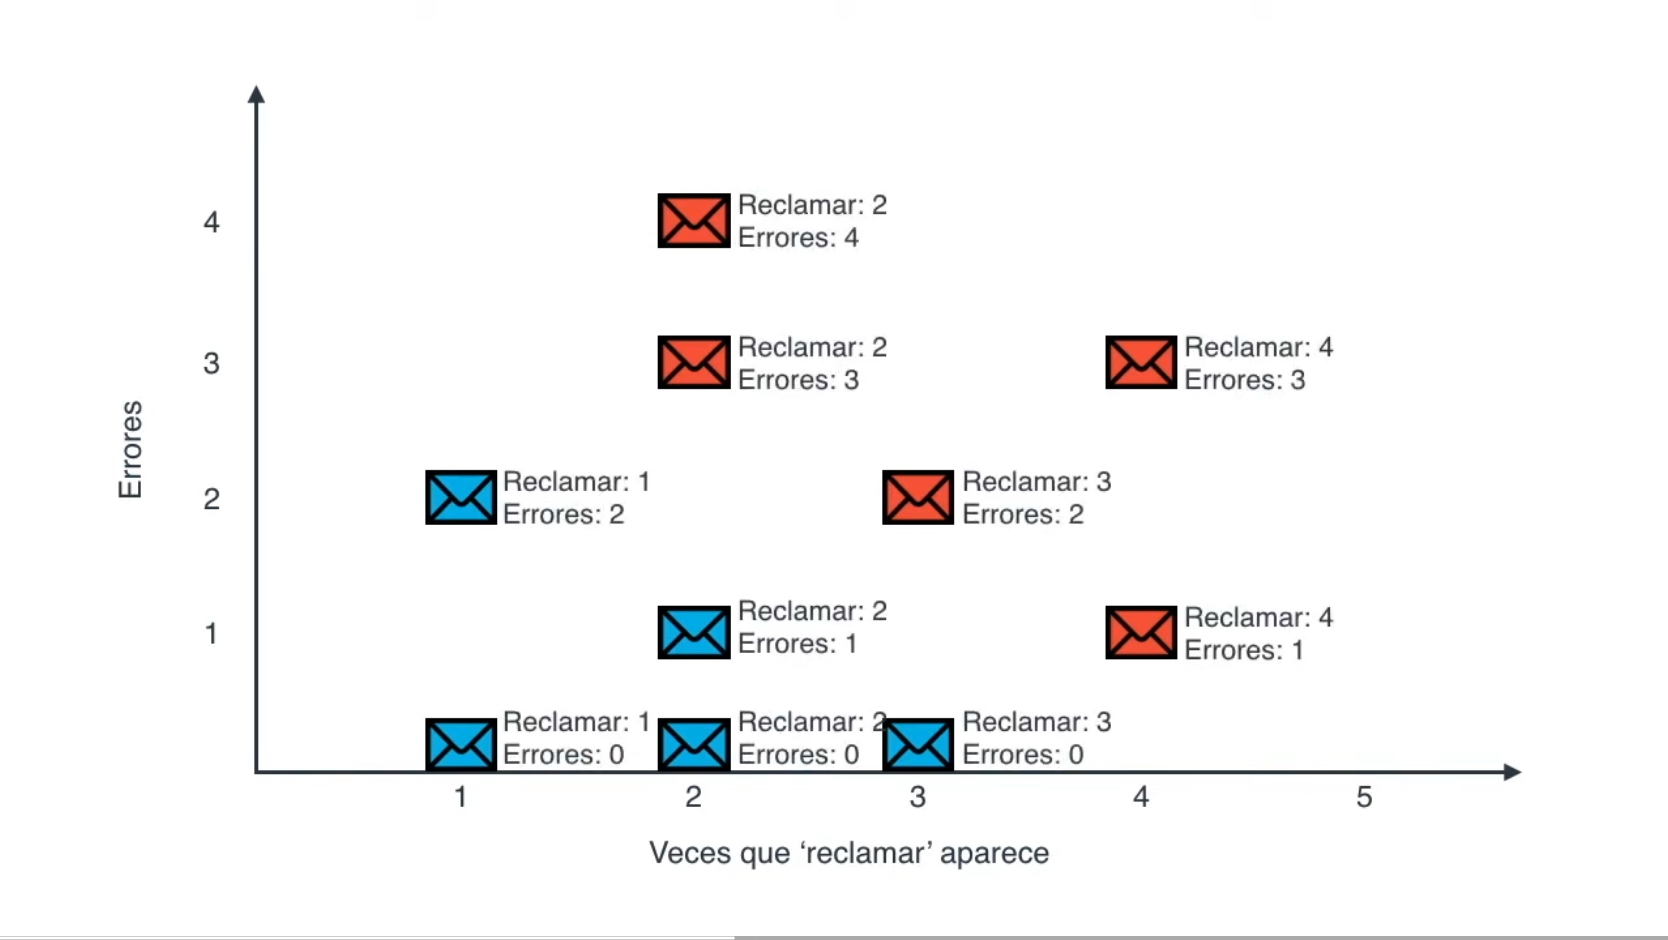
\includegraphics[width=0.9\textwidth]{Imagenes_reg_log/IMG_3499.jpg}
			\caption{https://serrano.academy/espanol/}
		\end{figure}
	\end{block}
\end{frame}

\begin{frame}
	\frametitle{MODELOS DE REGRESIÓN}
	\begin{block}{Regresión Logística}	
		\begin{figure}
			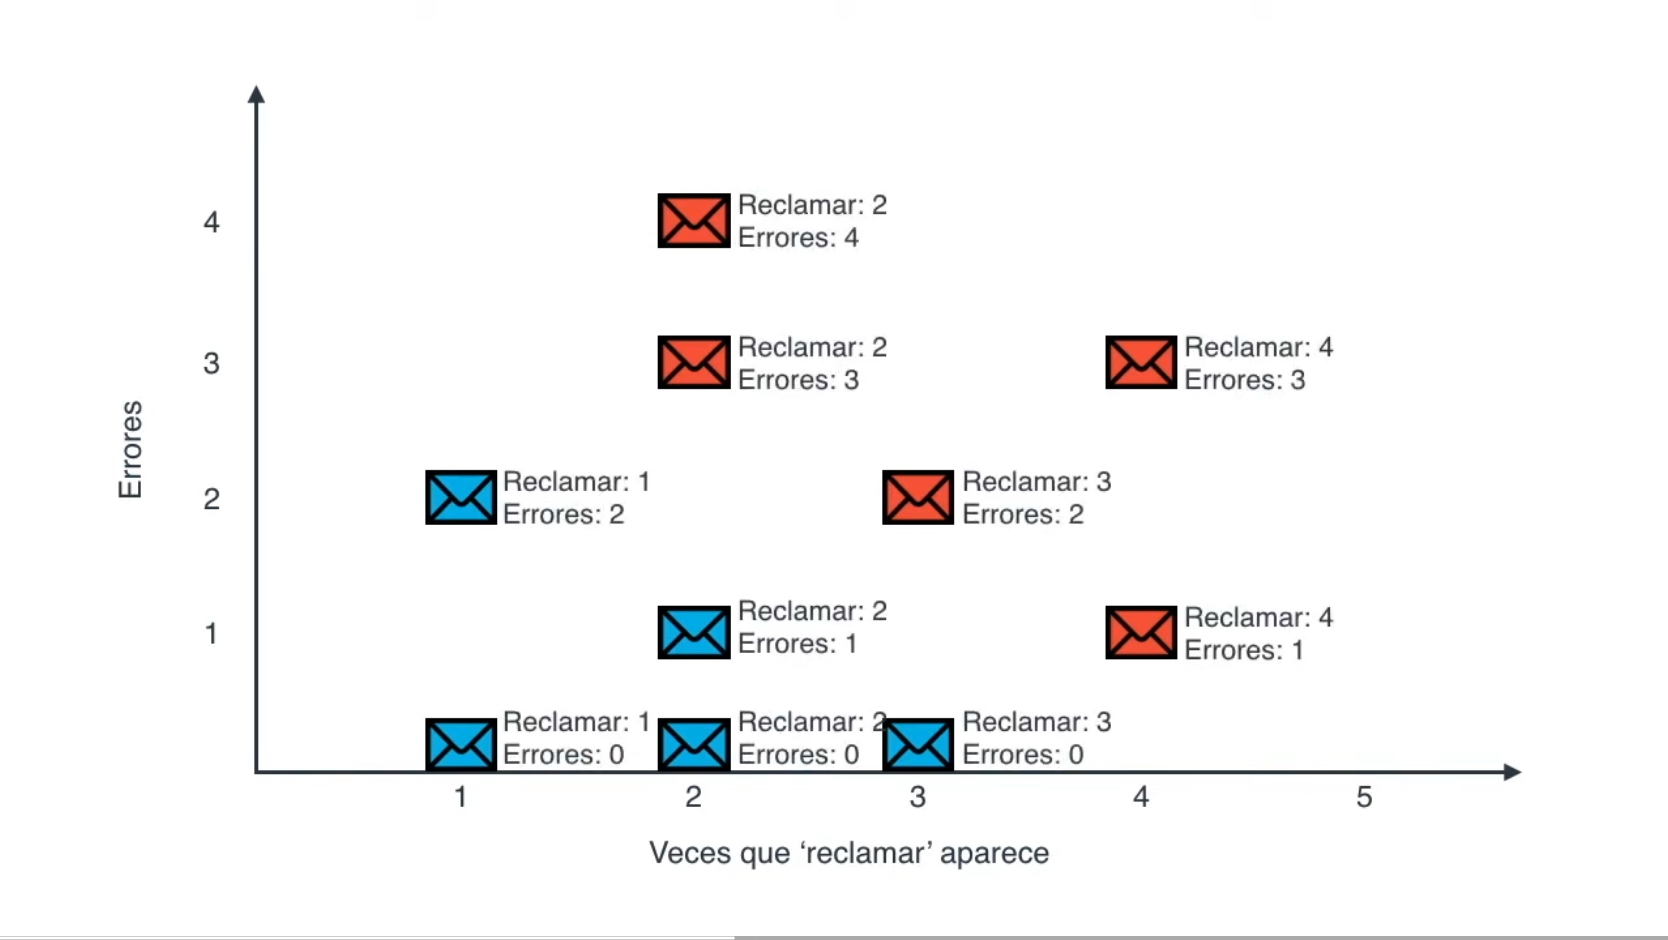
\includegraphics[width=0.9\textwidth]{Imagenes_reg_log/IMG_3499.jpg}
			\caption{https://serrano.academy/espanol/}
		\end{figure}
	\end{block}
\end{frame}

\begin{frame}
	\frametitle{MODELOS DE REGRESIÓN}
	\begin{block}{Regresión Logística}	
		\begin{figure}
			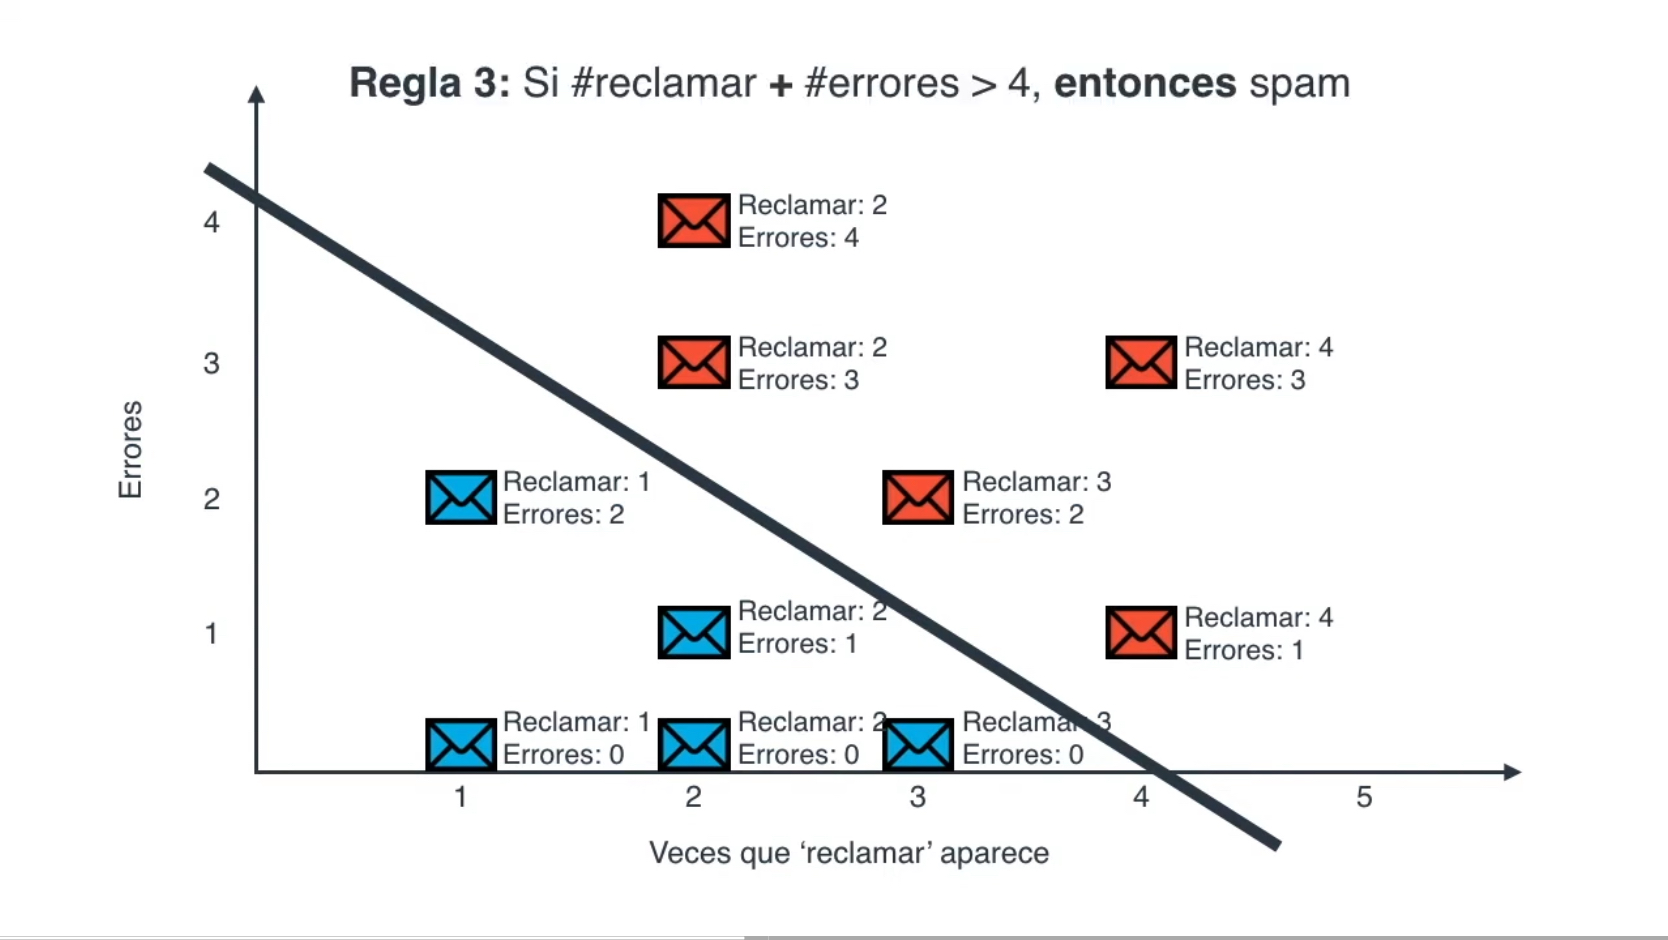
\includegraphics[width=0.9\textwidth]{Imagenes_reg_log/IMG_3500.jpg}
			\caption{https://serrano.academy/espanol/}
		\end{figure}
	\end{block}
\end{frame}

\begin{frame}
	\frametitle{MODELOS DE REGRESIÓN}
	\begin{block}{Regresión Logística}	
		\begin{figure}
			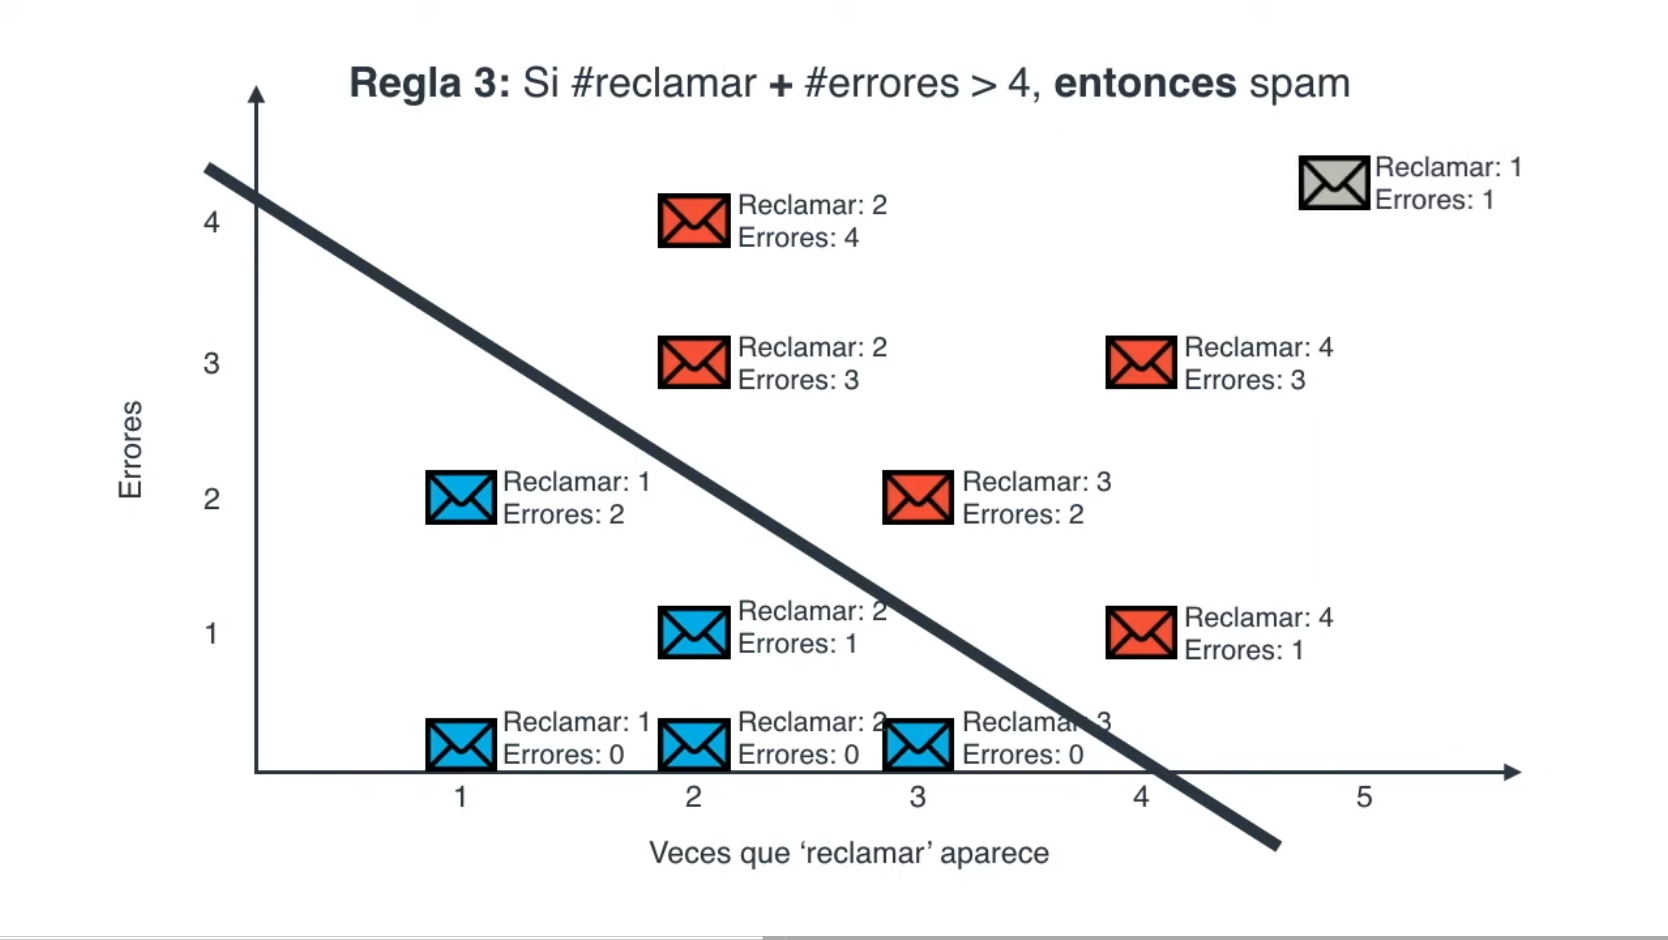
\includegraphics[width=0.9\textwidth]{Imagenes_reg_log/IMG_3502.jpg}
			\caption{https://serrano.academy/espanol/}
		\end{figure}
	\end{block}
\end{frame}

 \begin{frame}
 	\frametitle{MODELOS DE REGRESIÓN}
 	\begin{block}{Regresión Logística}	
 		\begin{figure}
 			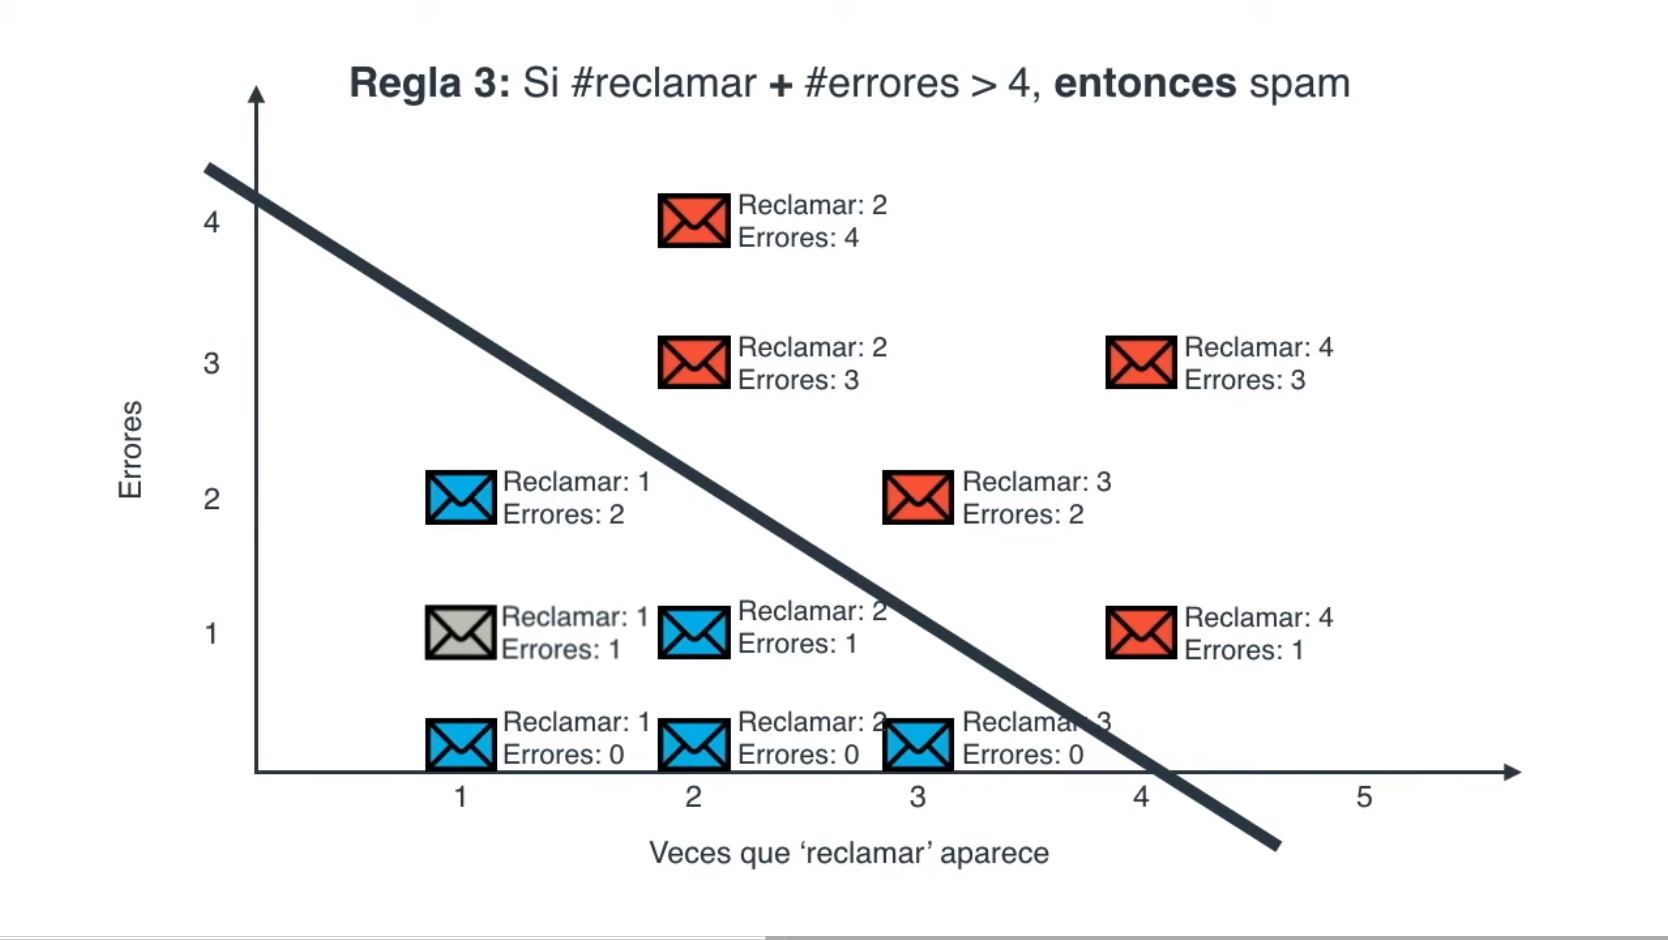
\includegraphics[width=0.9\textwidth]{Imagenes_reg_log/IMG_3503.jpg}
 			\caption{https://serrano.academy/espanol/}
 		\end{figure}
 	\end{block}
 \end{frame}

\begin{frame}
	\frametitle{MODELOS DE REGRESIÓN}
	\begin{block}{Regresión Logística}	
		\begin{figure}
			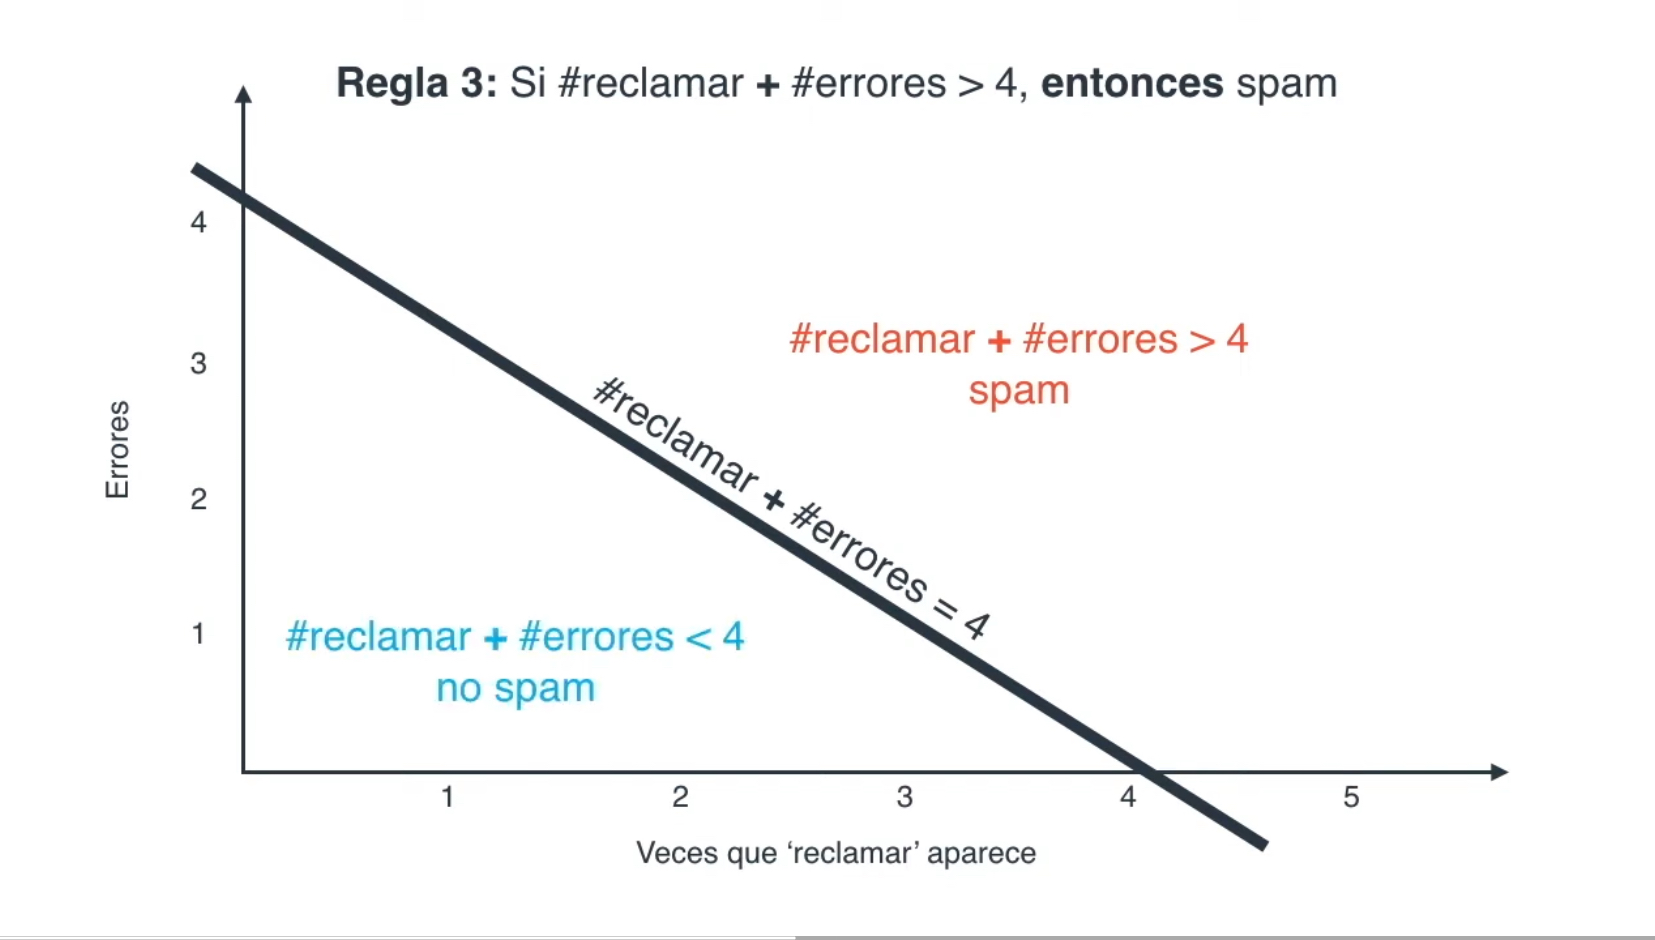
\includegraphics[width=0.9\textwidth]{Imagenes_reg_log/IMG_3504.jpg}
			\caption{https://serrano.academy/espanol/}
		\end{figure}
	\end{block}
\end{frame}

\section{MODELOS DE K-MEDIAS}

\begin{frame}
	\frametitle{MODELOS DE APRENDIZAJE DE MÁQUINA}
	\begin{block}{}	
		\center
		\textbf{MODELO DE K-MEDIAS}
	\end{block}
\end{frame}


\begin{frame}
	\frametitle{MÉTODOS NO SUPERVISADOS}
	\begin{block}{K Medias}	
		\begin{figure}
			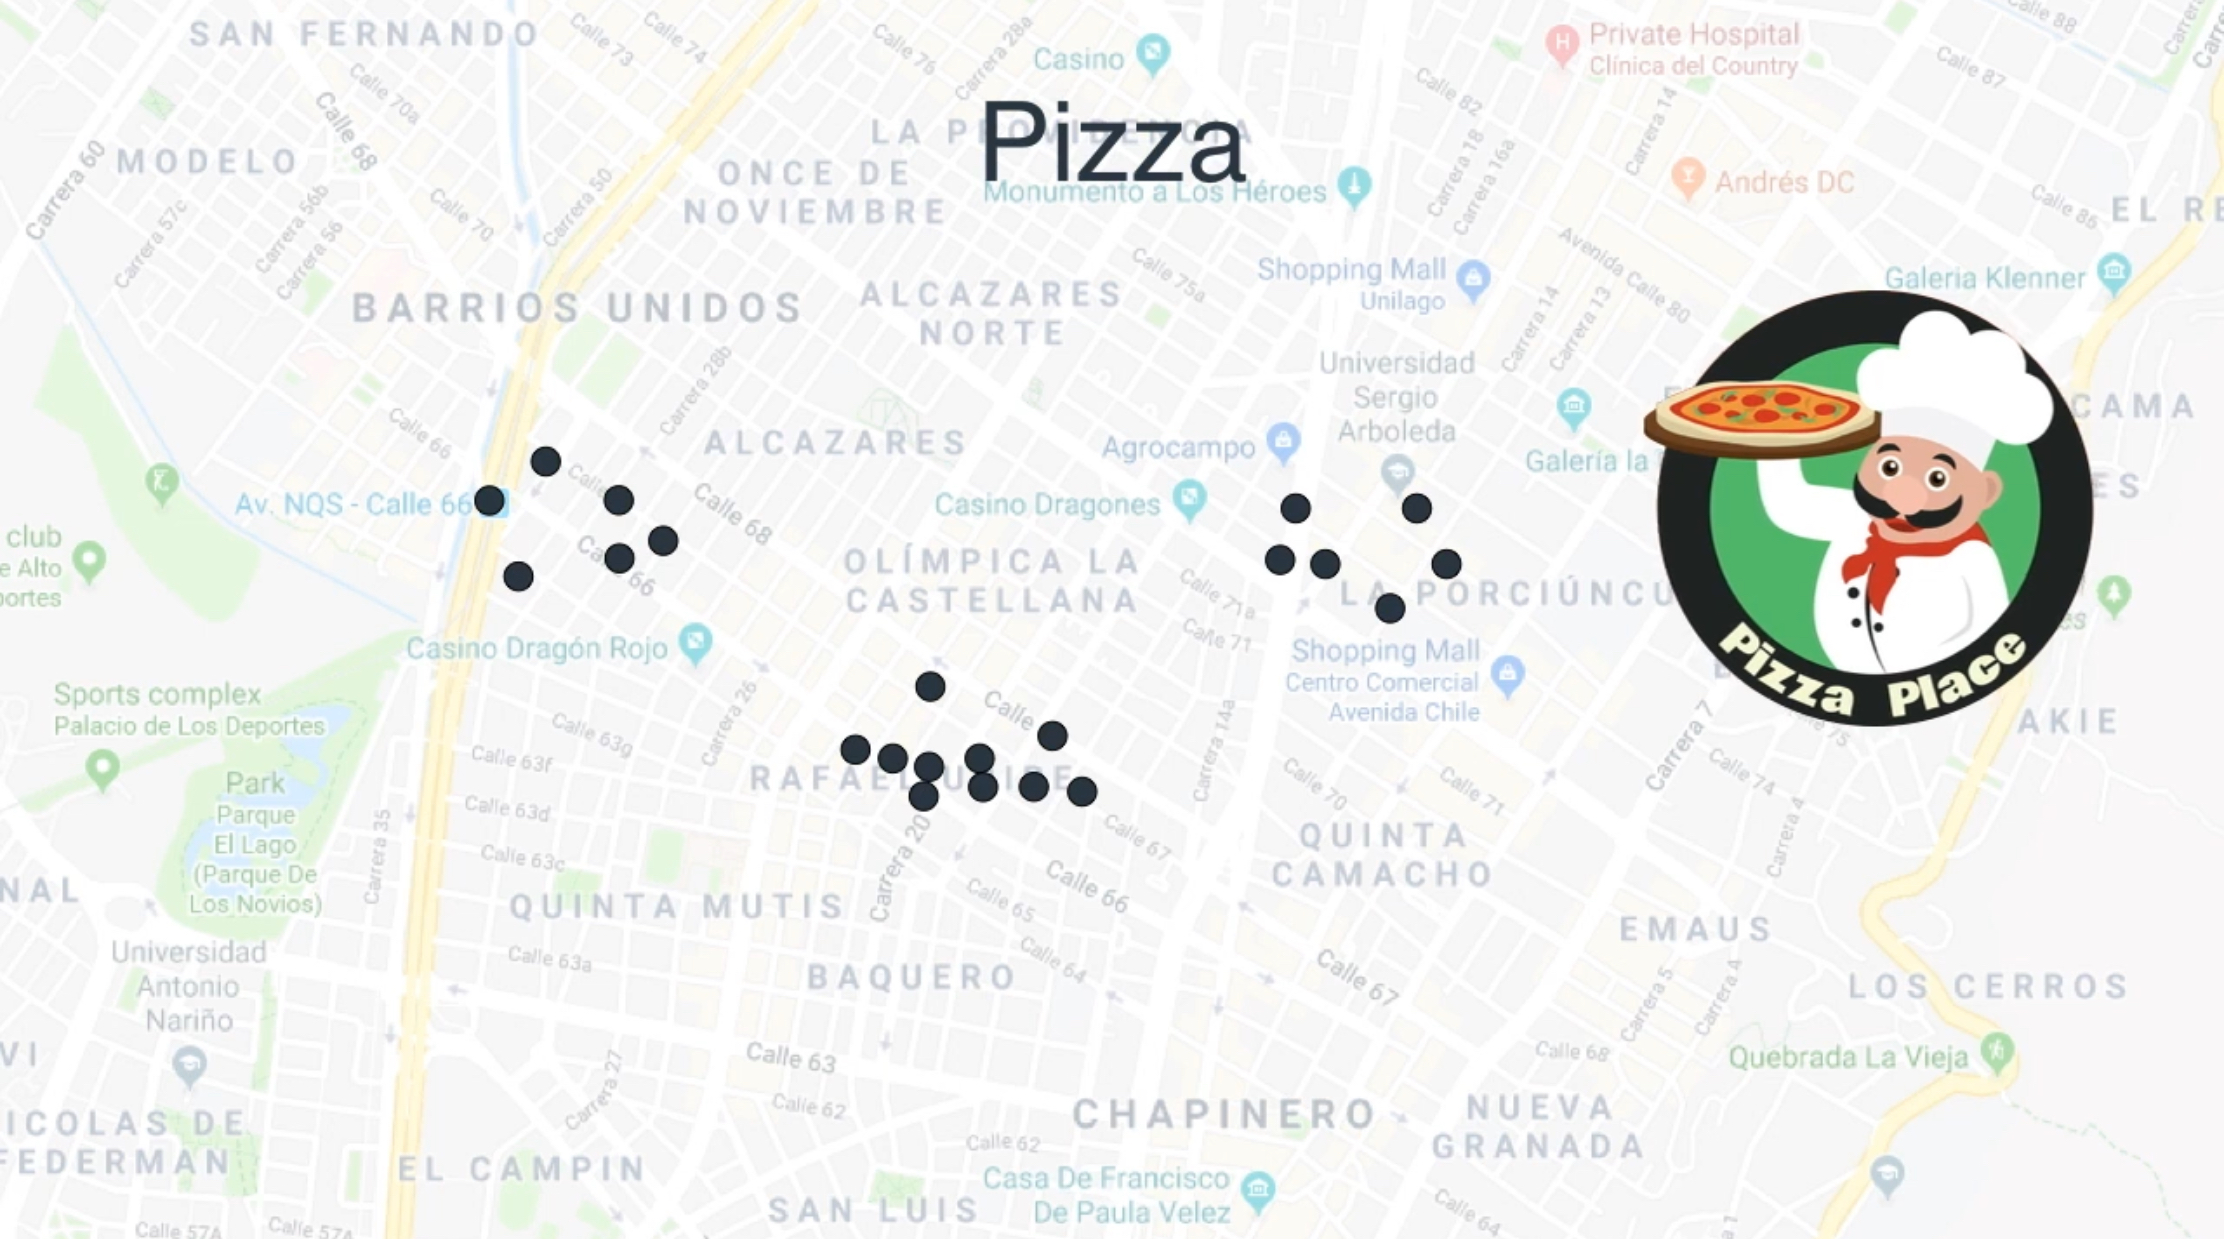
\includegraphics[width=0.9\textwidth]{Imagenes_k_means/IMG_3506.jpg}
			\caption{https://serrano.academy/espanol/}
		\end{figure}
	\end{block}
\end{frame}

\begin{frame}
	\frametitle{MÉTODOS NO SUPERVISADOS}
	\begin{block}{K Medias}	
		\begin{figure}
			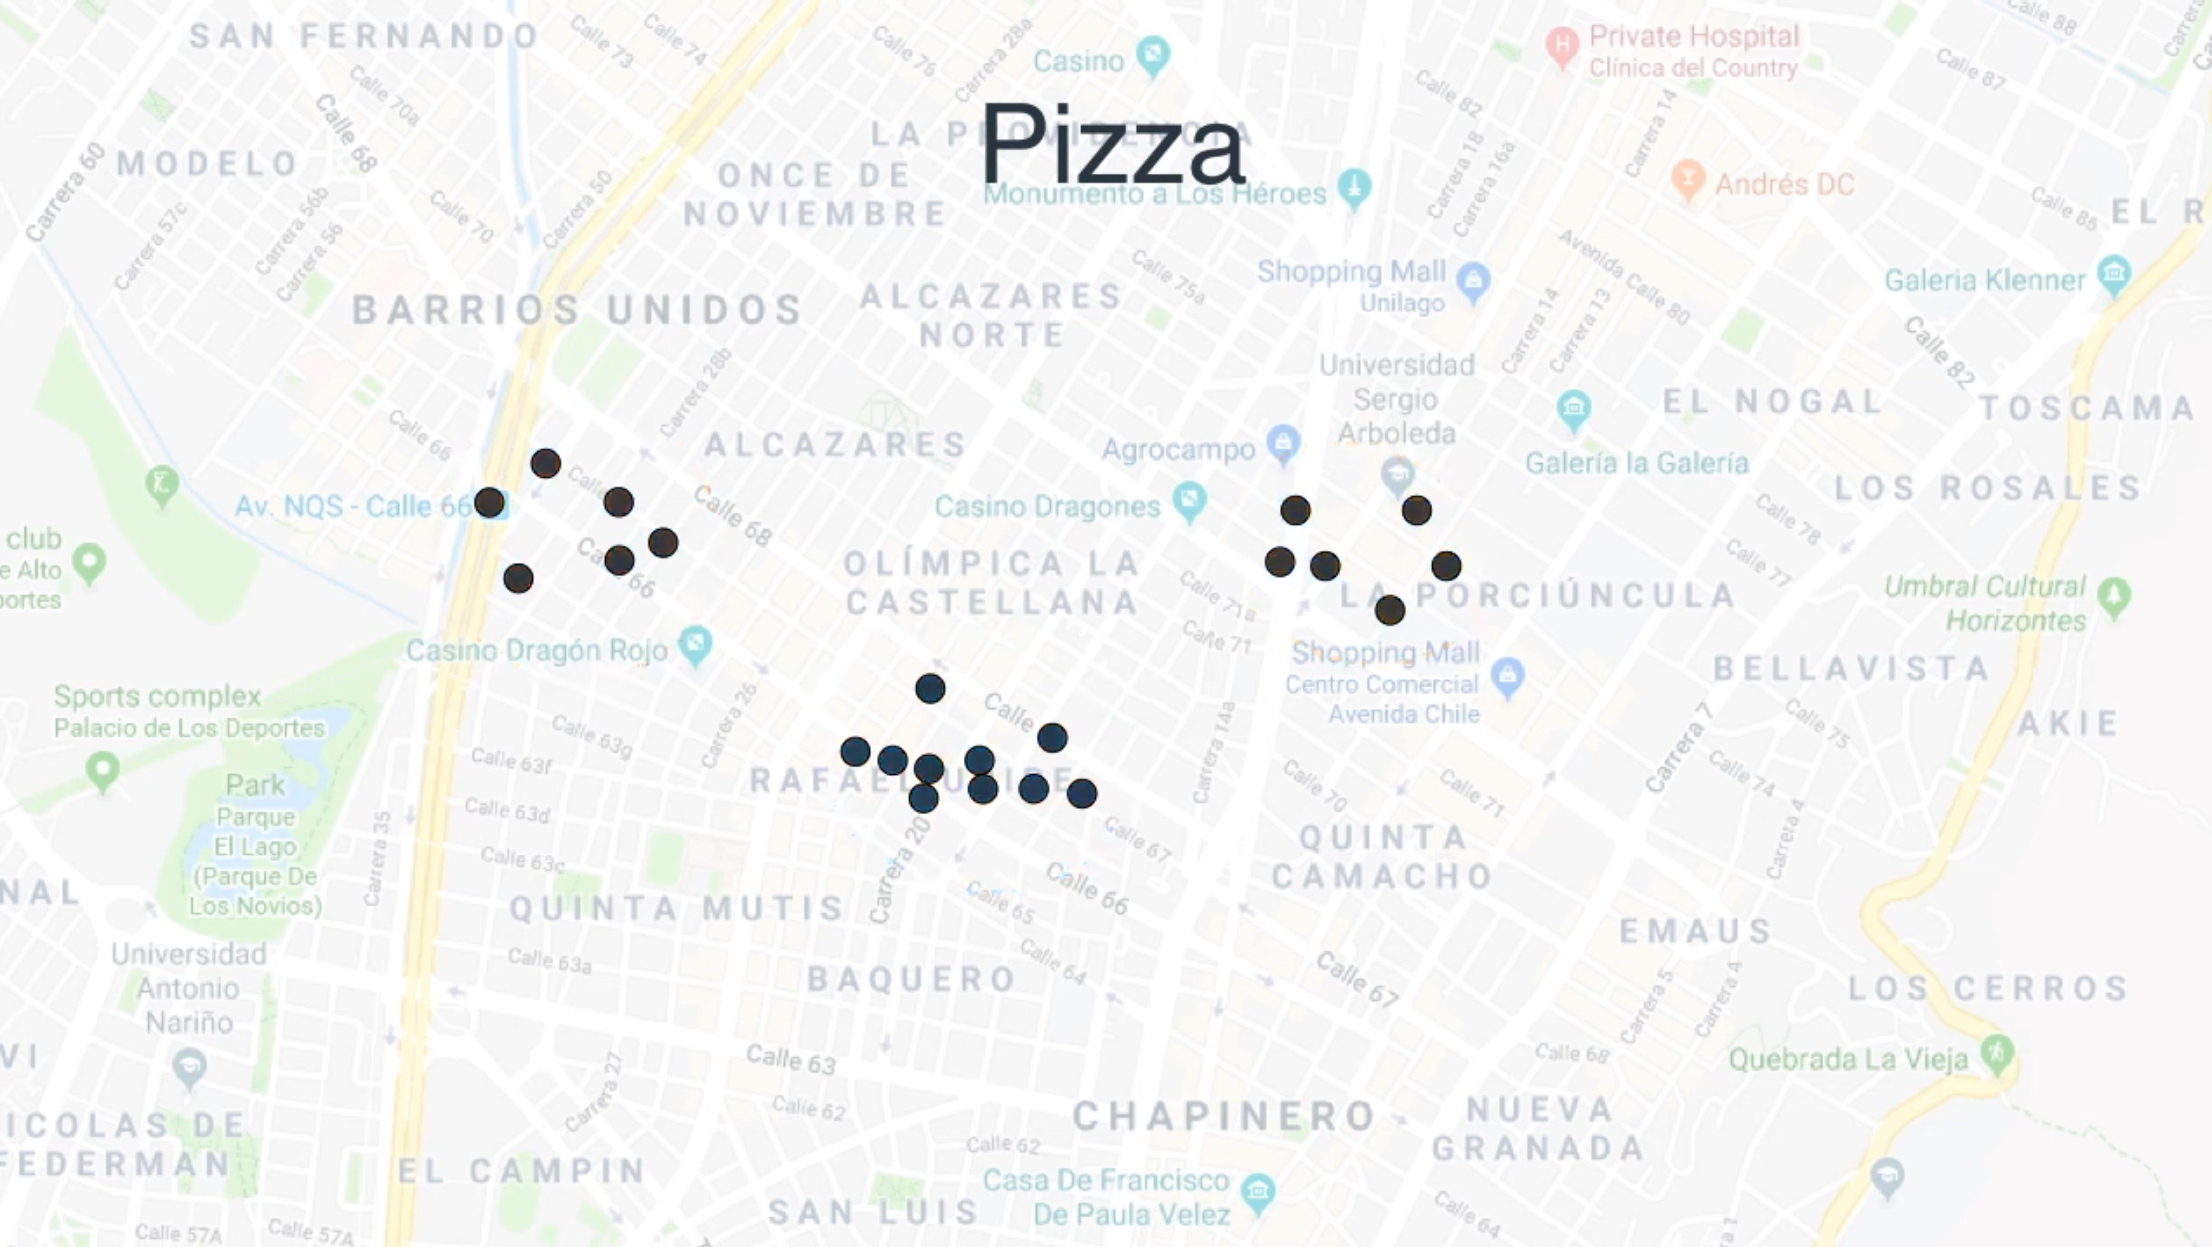
\includegraphics[width=0.9\textwidth]{Imagenes_k_means/IMG_3507.jpg}
			\caption{https://serrano.academy/espanol/}
		\end{figure}
	\end{block}
\end{frame}

 \begin{frame}
 	\frametitle{MÉTODOS NO SUPERVISADOS}
 	\begin{block}{K Medias}	
 		\begin{figure}
 			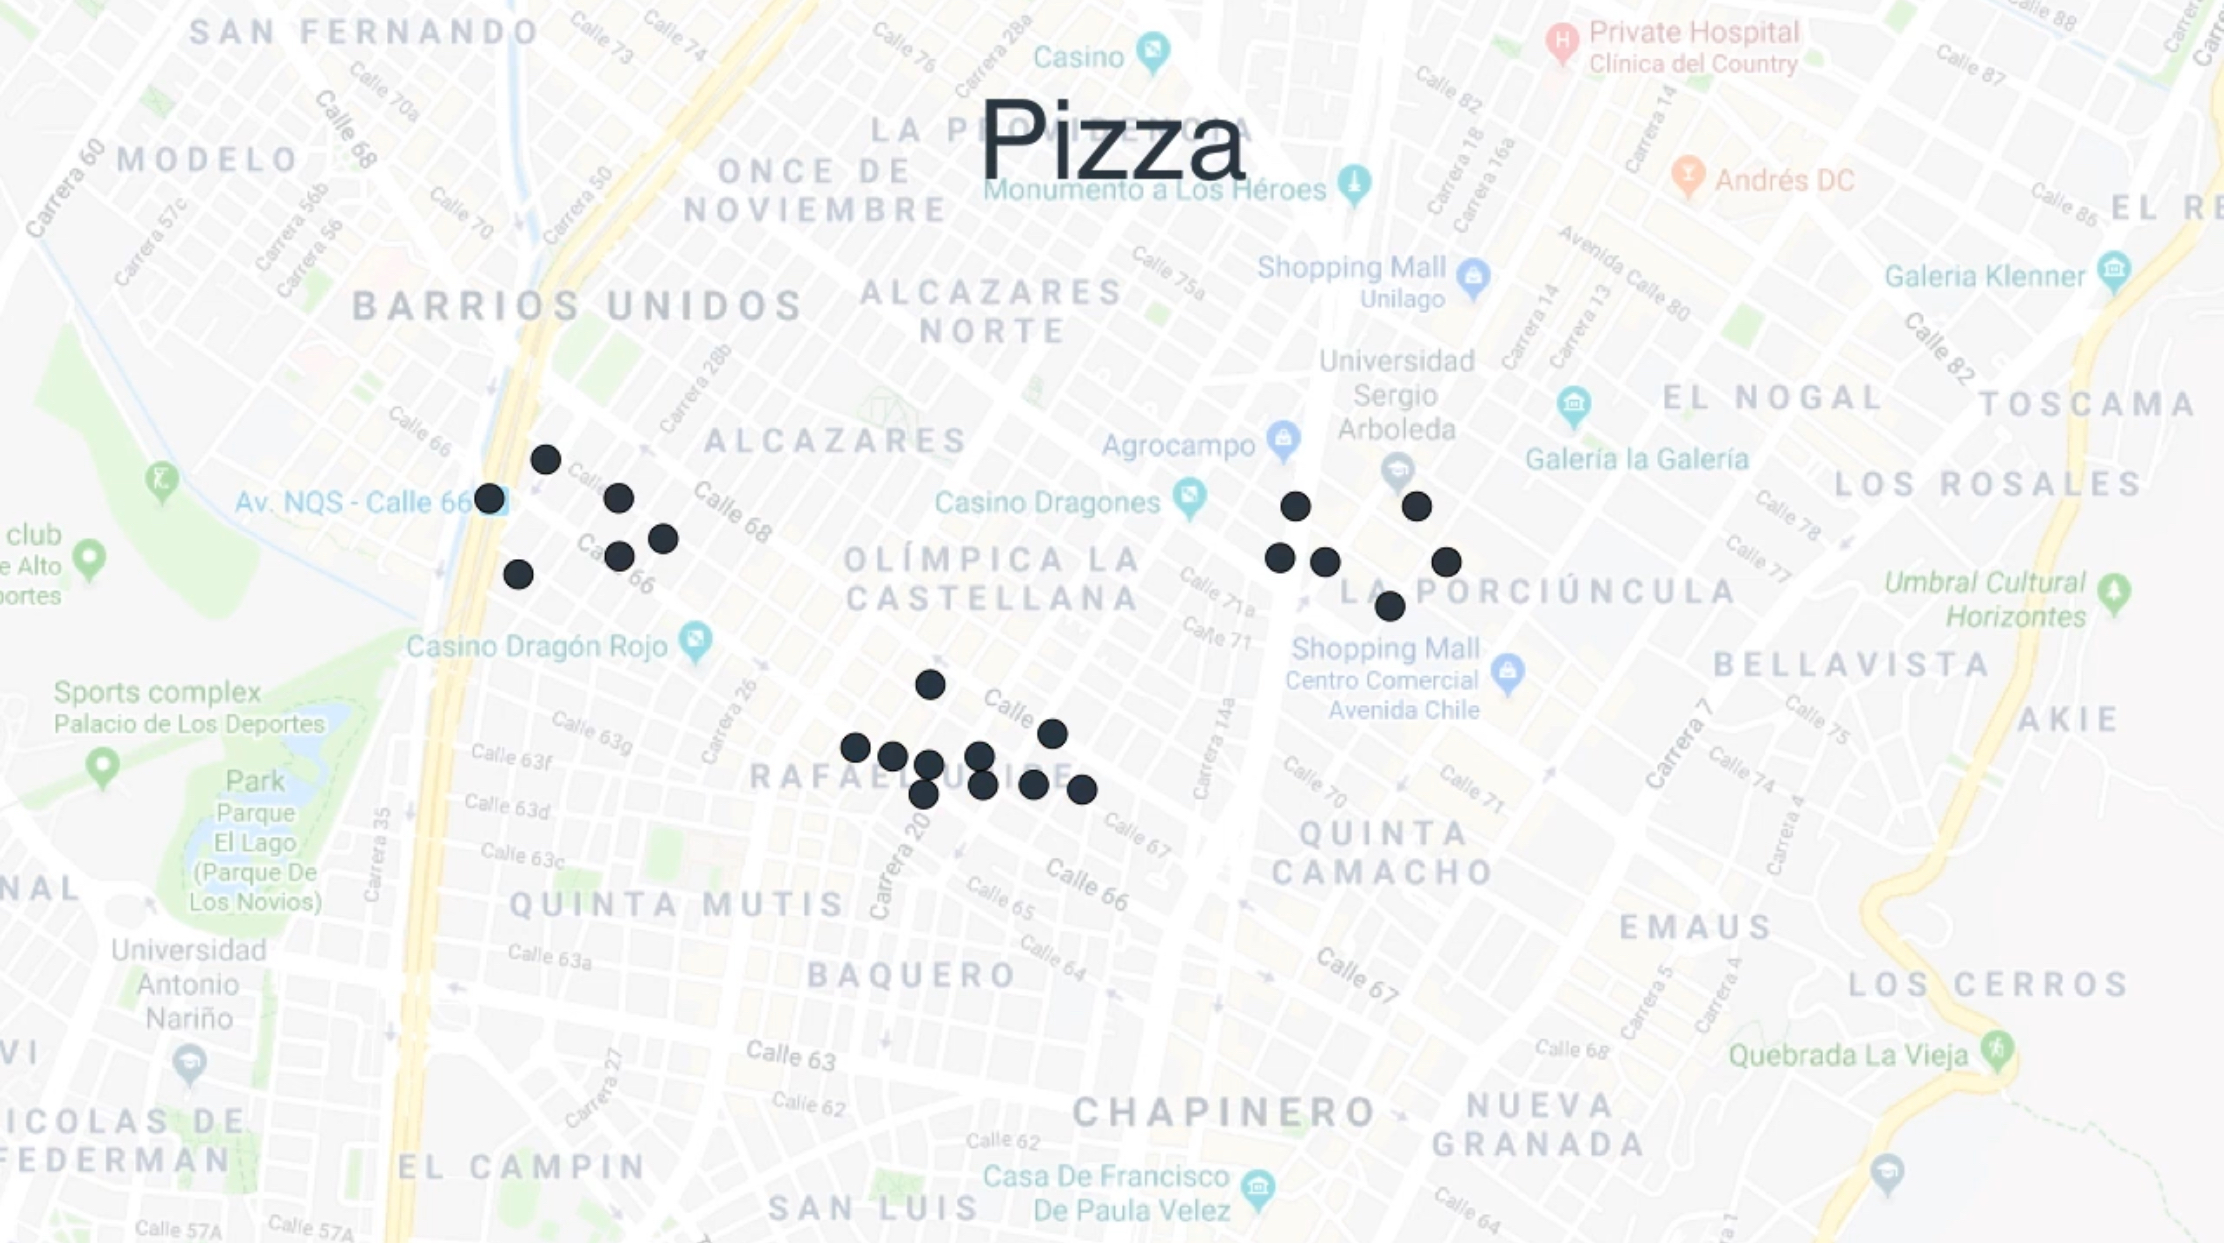
\includegraphics[width=0.9\textwidth]{Imagenes_k_means/IMG_3508.jpg}
 			\caption{https://serrano.academy/espanol/}
 		\end{figure}
 	\end{block}
 \end{frame}

\begin{frame}
	\frametitle{MÉTODOS NO SUPERVISADOS}
	\begin{block}{K Medias}	
		\begin{figure}
			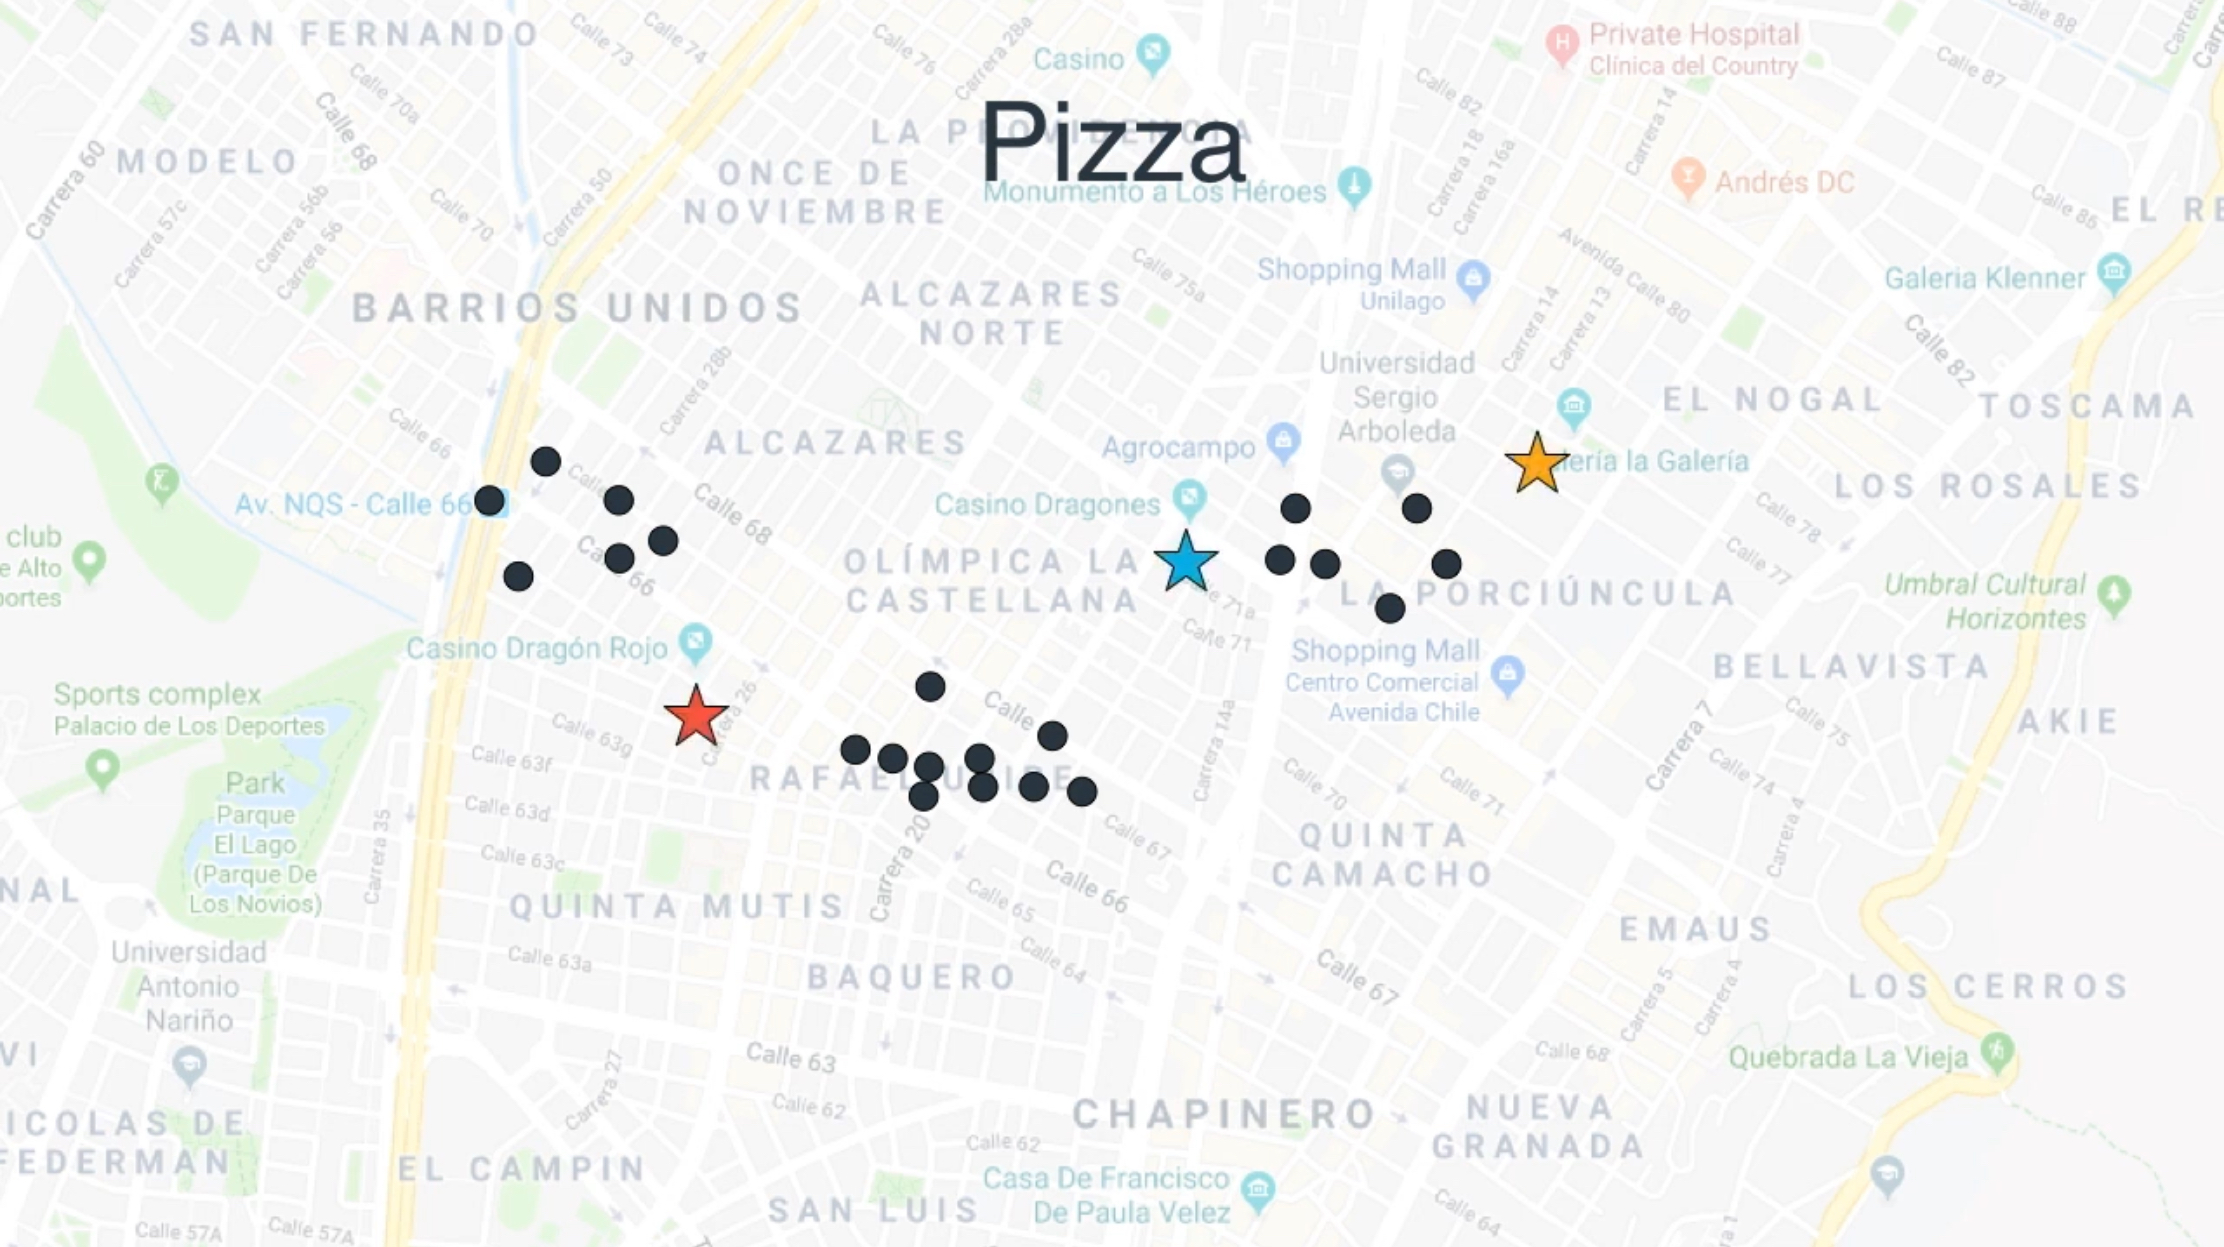
\includegraphics[width=0.9\textwidth]{Imagenes_k_means/IMG_3509.jpg}
			\caption{https://serrano.academy/espanol/}
		\end{figure}
	\end{block}
\end{frame}

\begin{frame}
	\frametitle{MÉTODOS NO SUPERVISADOS}
	\begin{block}{K Medias}	
		\begin{figure}
			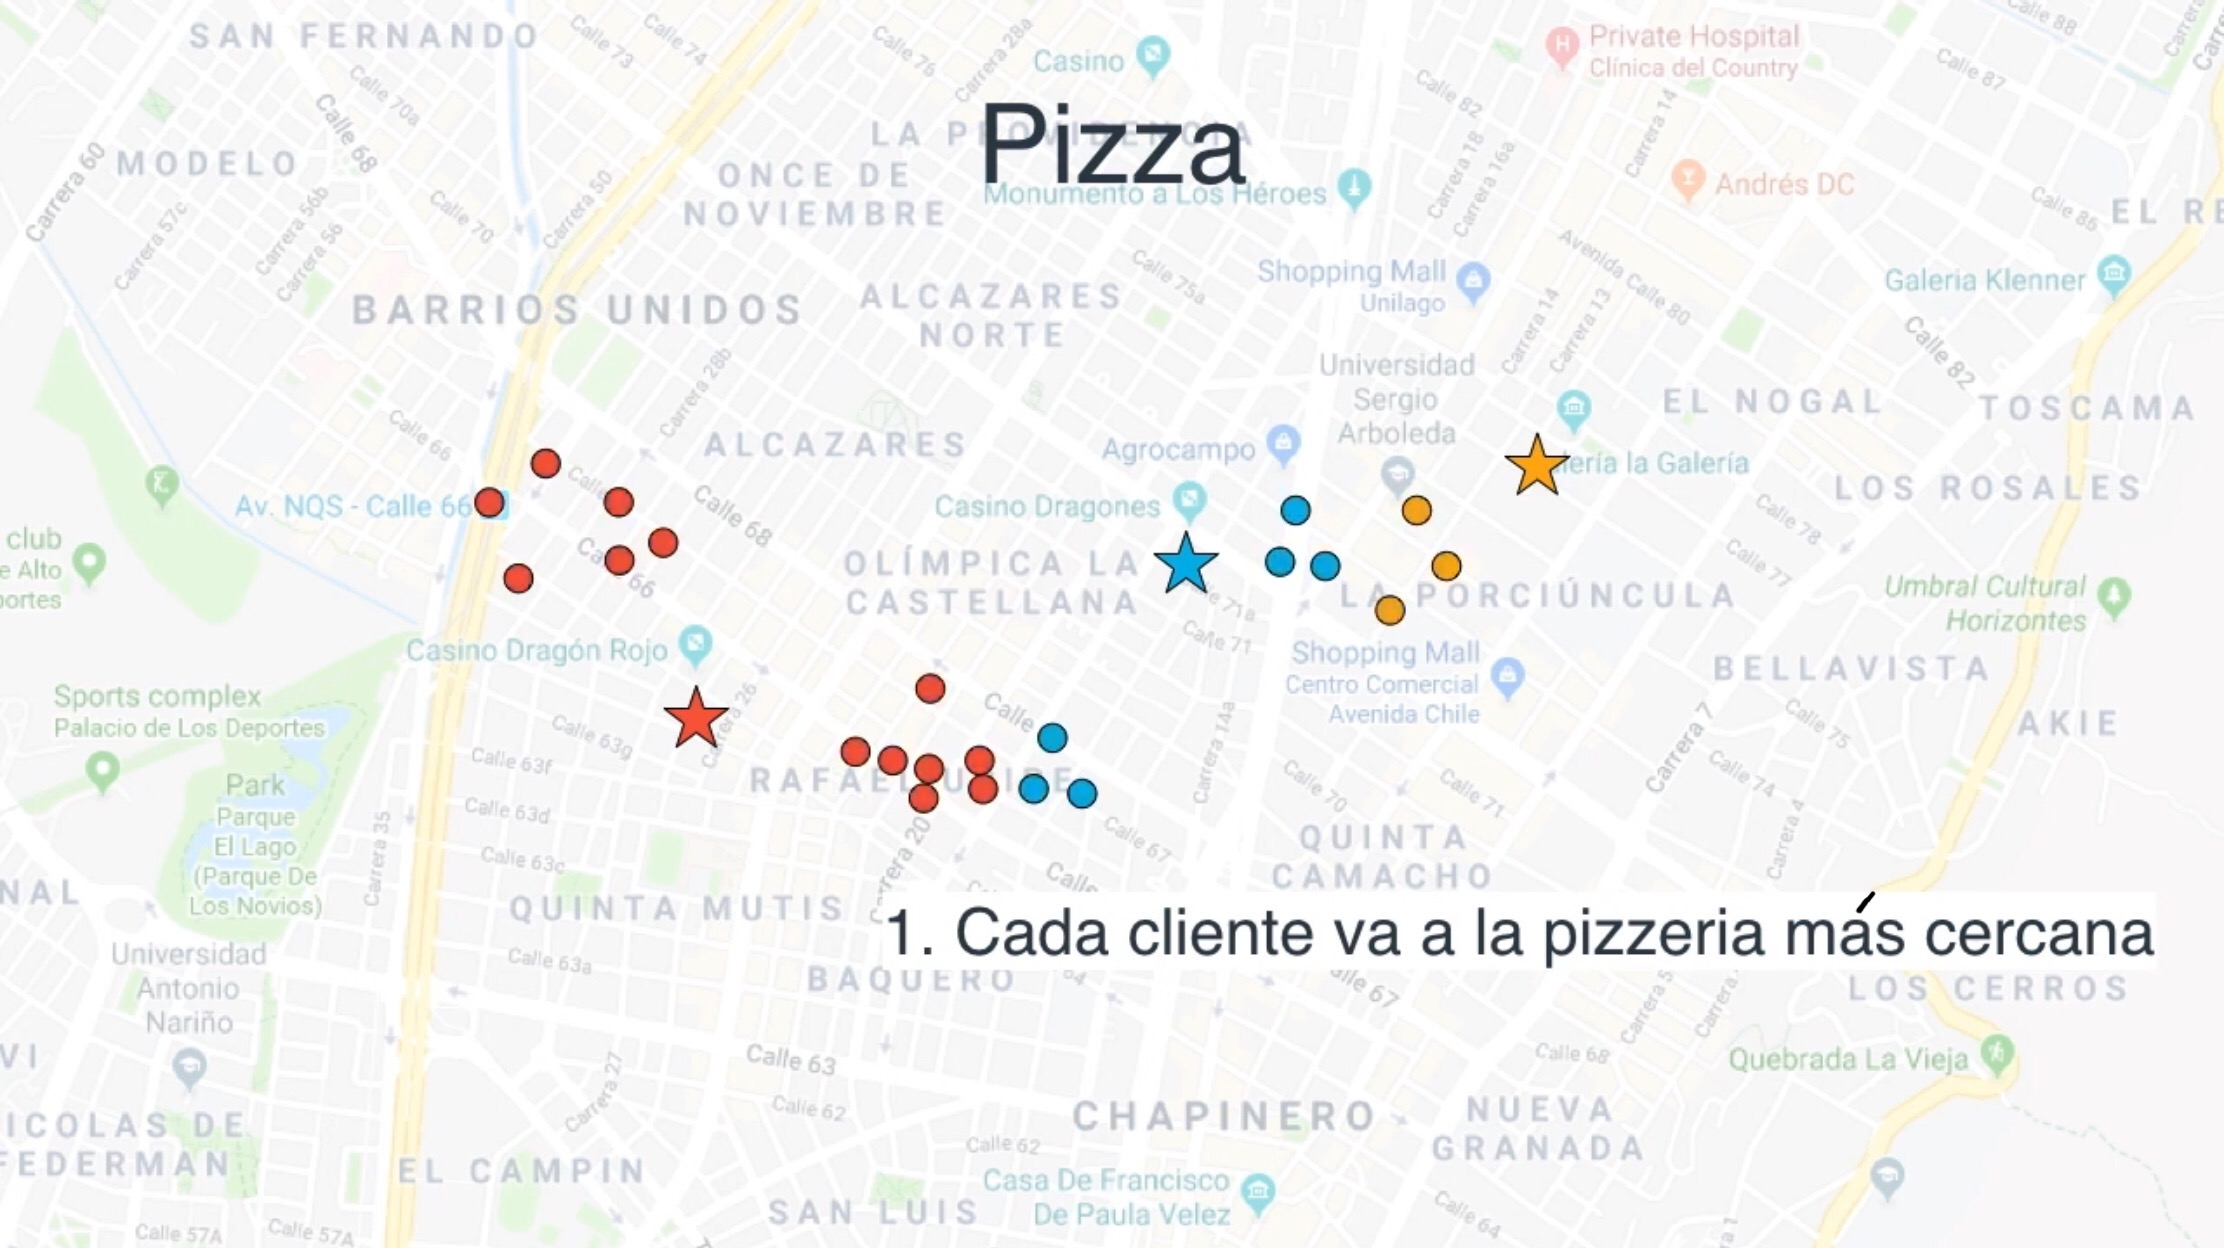
\includegraphics[width=0.9\textwidth]{Imagenes_k_means/IMG_3510.jpg}
			\caption{https://serrano.academy/espanol/}
		\end{figure}
	\end{block}
\end{frame}


\begin{frame}
	\frametitle{MÉTODOS NO SUPERVISADOS}
	\begin{block}{K Medias}	
		\begin{figure}
			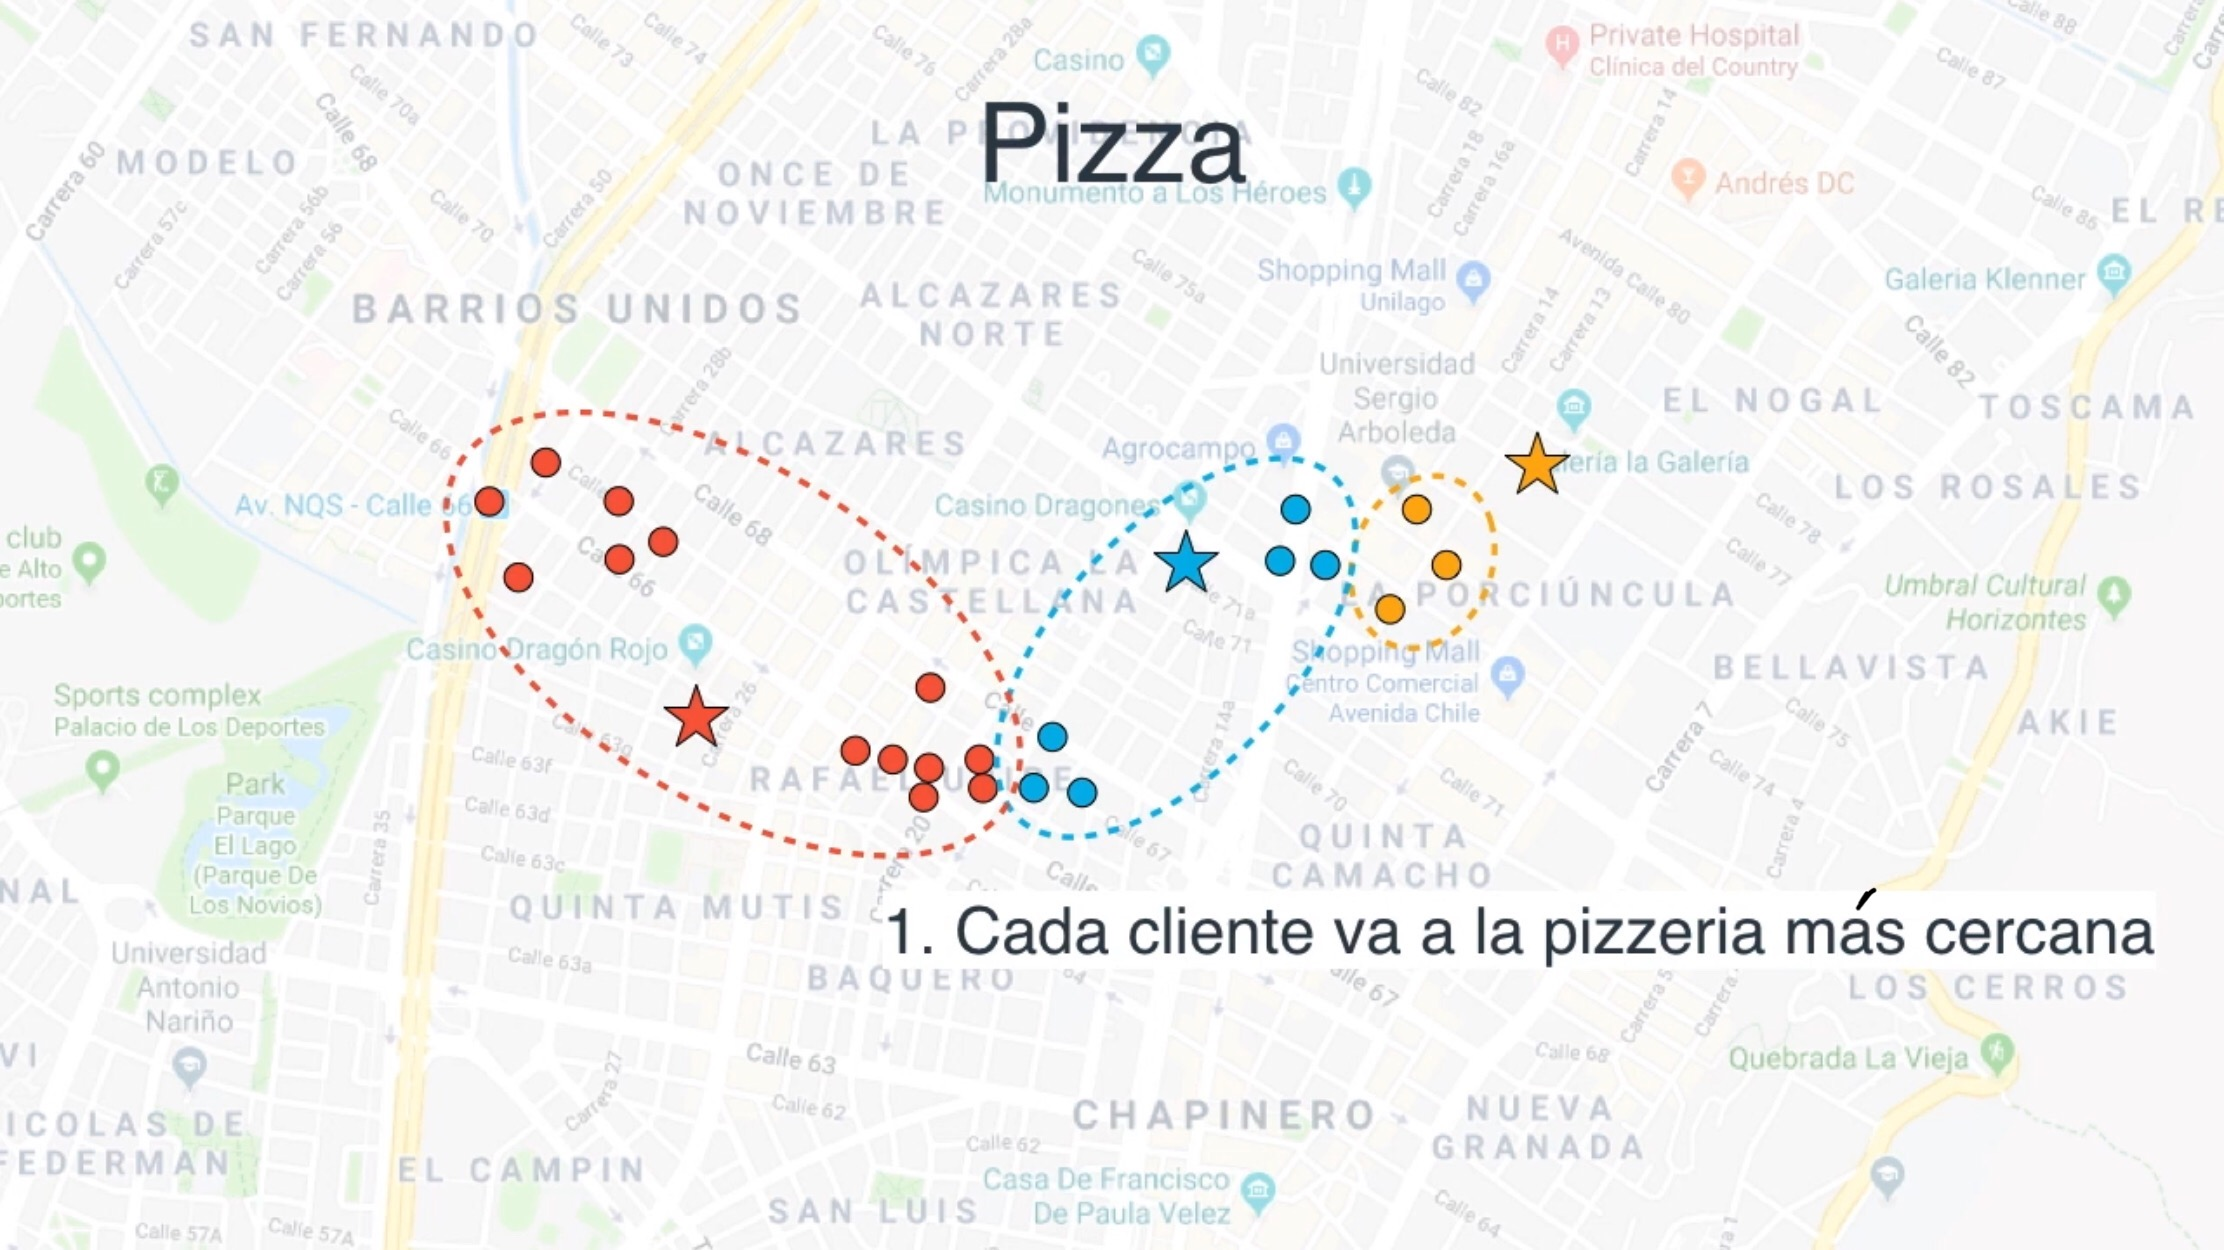
\includegraphics[width=0.9\textwidth]{Imagenes_k_means/IMG_3511.jpg}
			\caption{https://serrano.academy/espanol/}
		\end{figure}
	\end{block}
\end{frame}


\begin{frame}
	\frametitle{MÉTODOS NO SUPERVISADOS}
	\begin{block}{K Medias}	
		\begin{figure}
			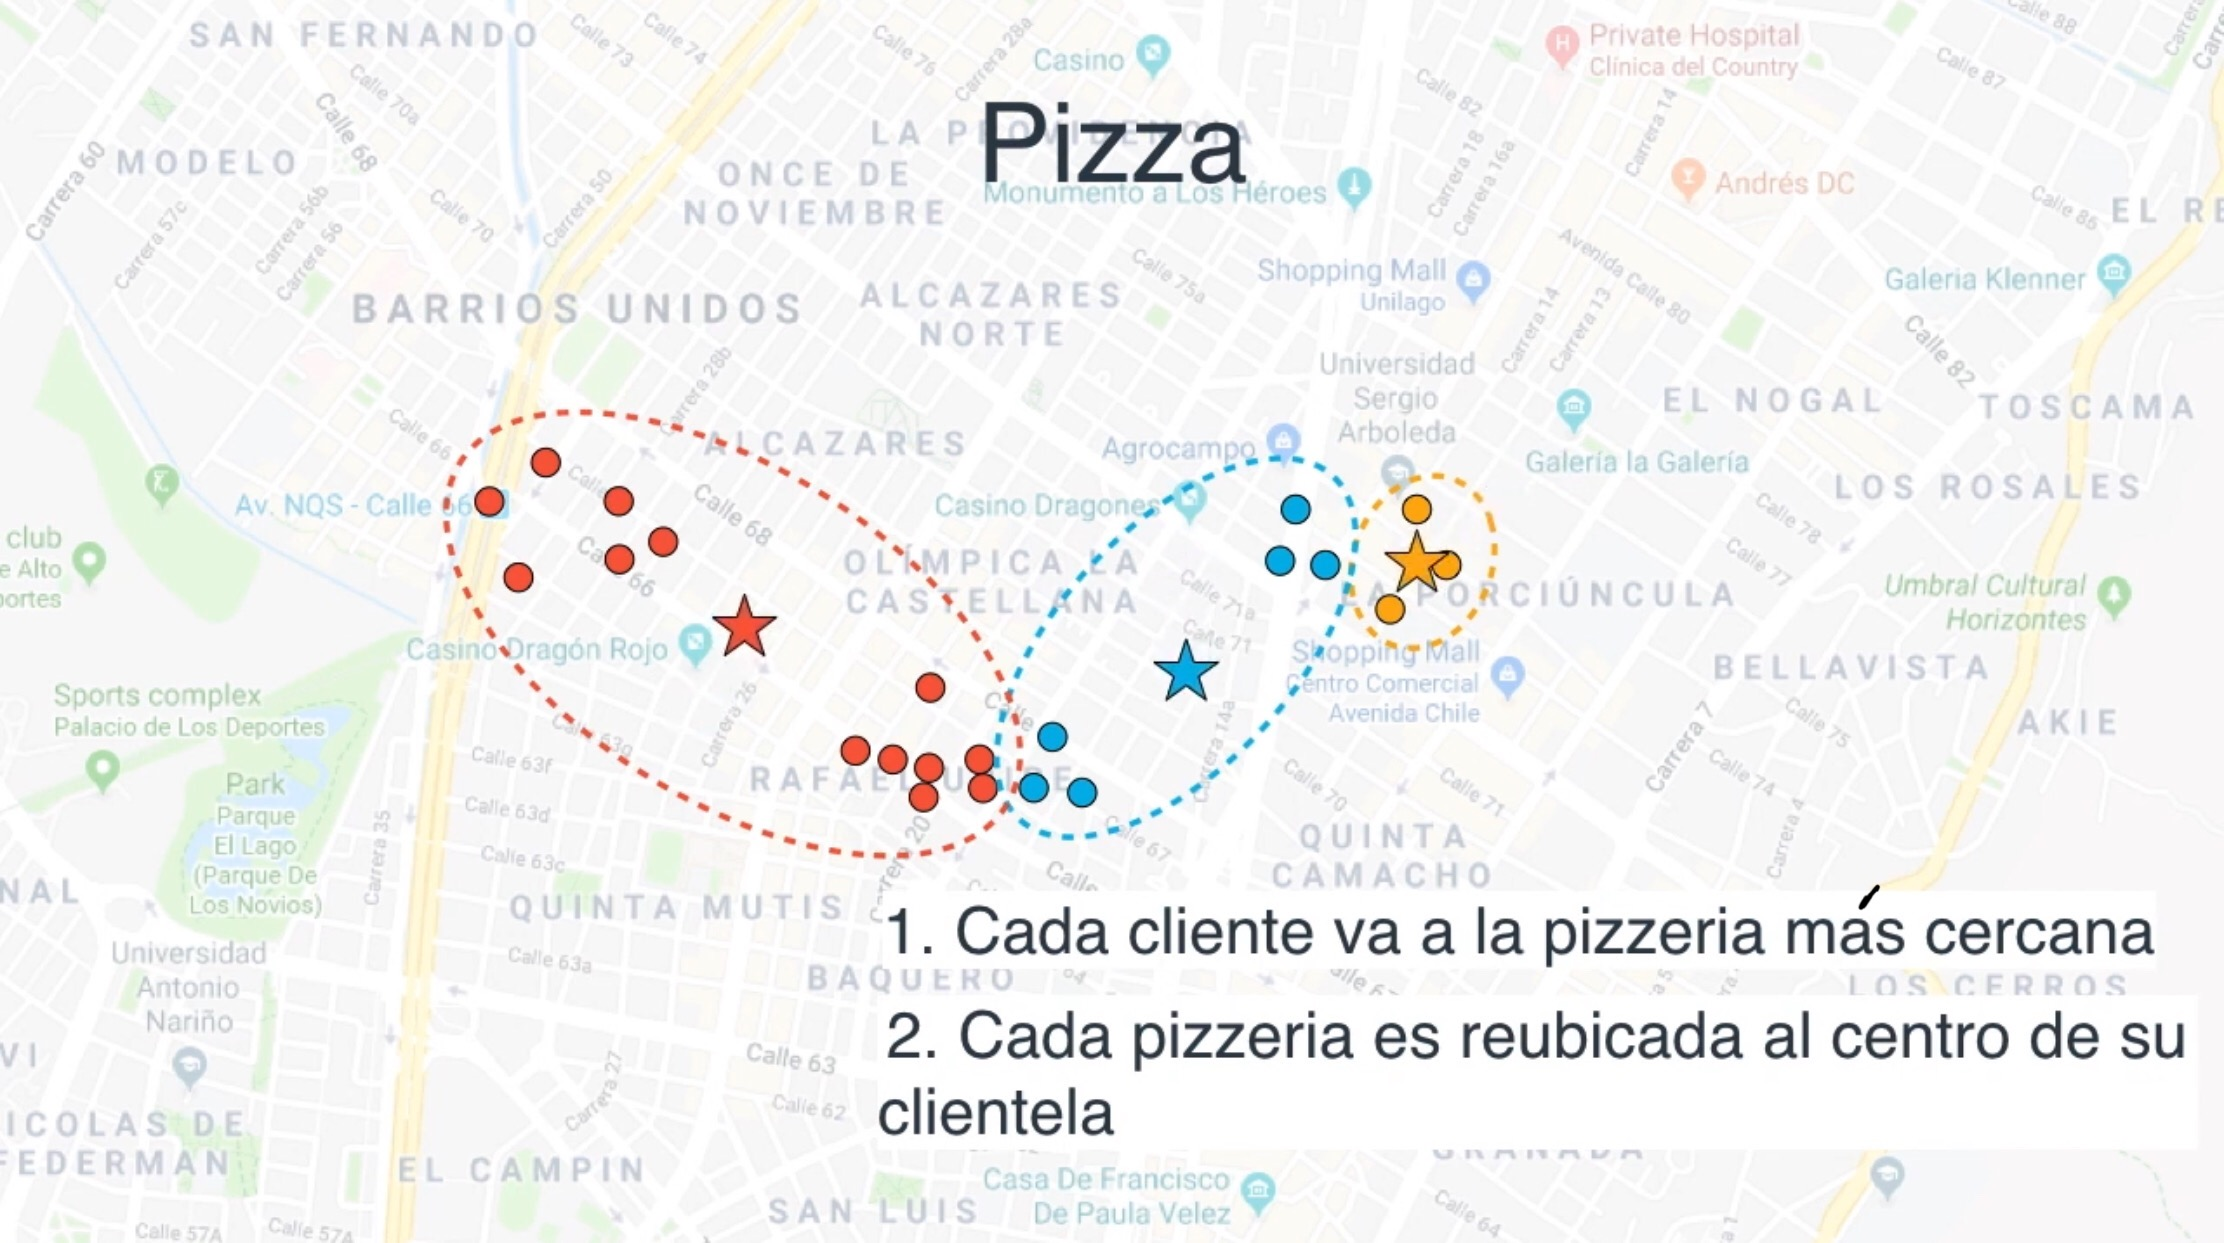
\includegraphics[width=0.9\textwidth]{Imagenes_k_means/IMG_3512.jpg}
			\caption{https://serrano.academy/espanol/}
		\end{figure}
	\end{block}
\end{frame}

\begin{frame}
	\frametitle{MÉTODOS NO SUPERVISADOS}
	\begin{block}{K Medias}	
		\begin{figure}
			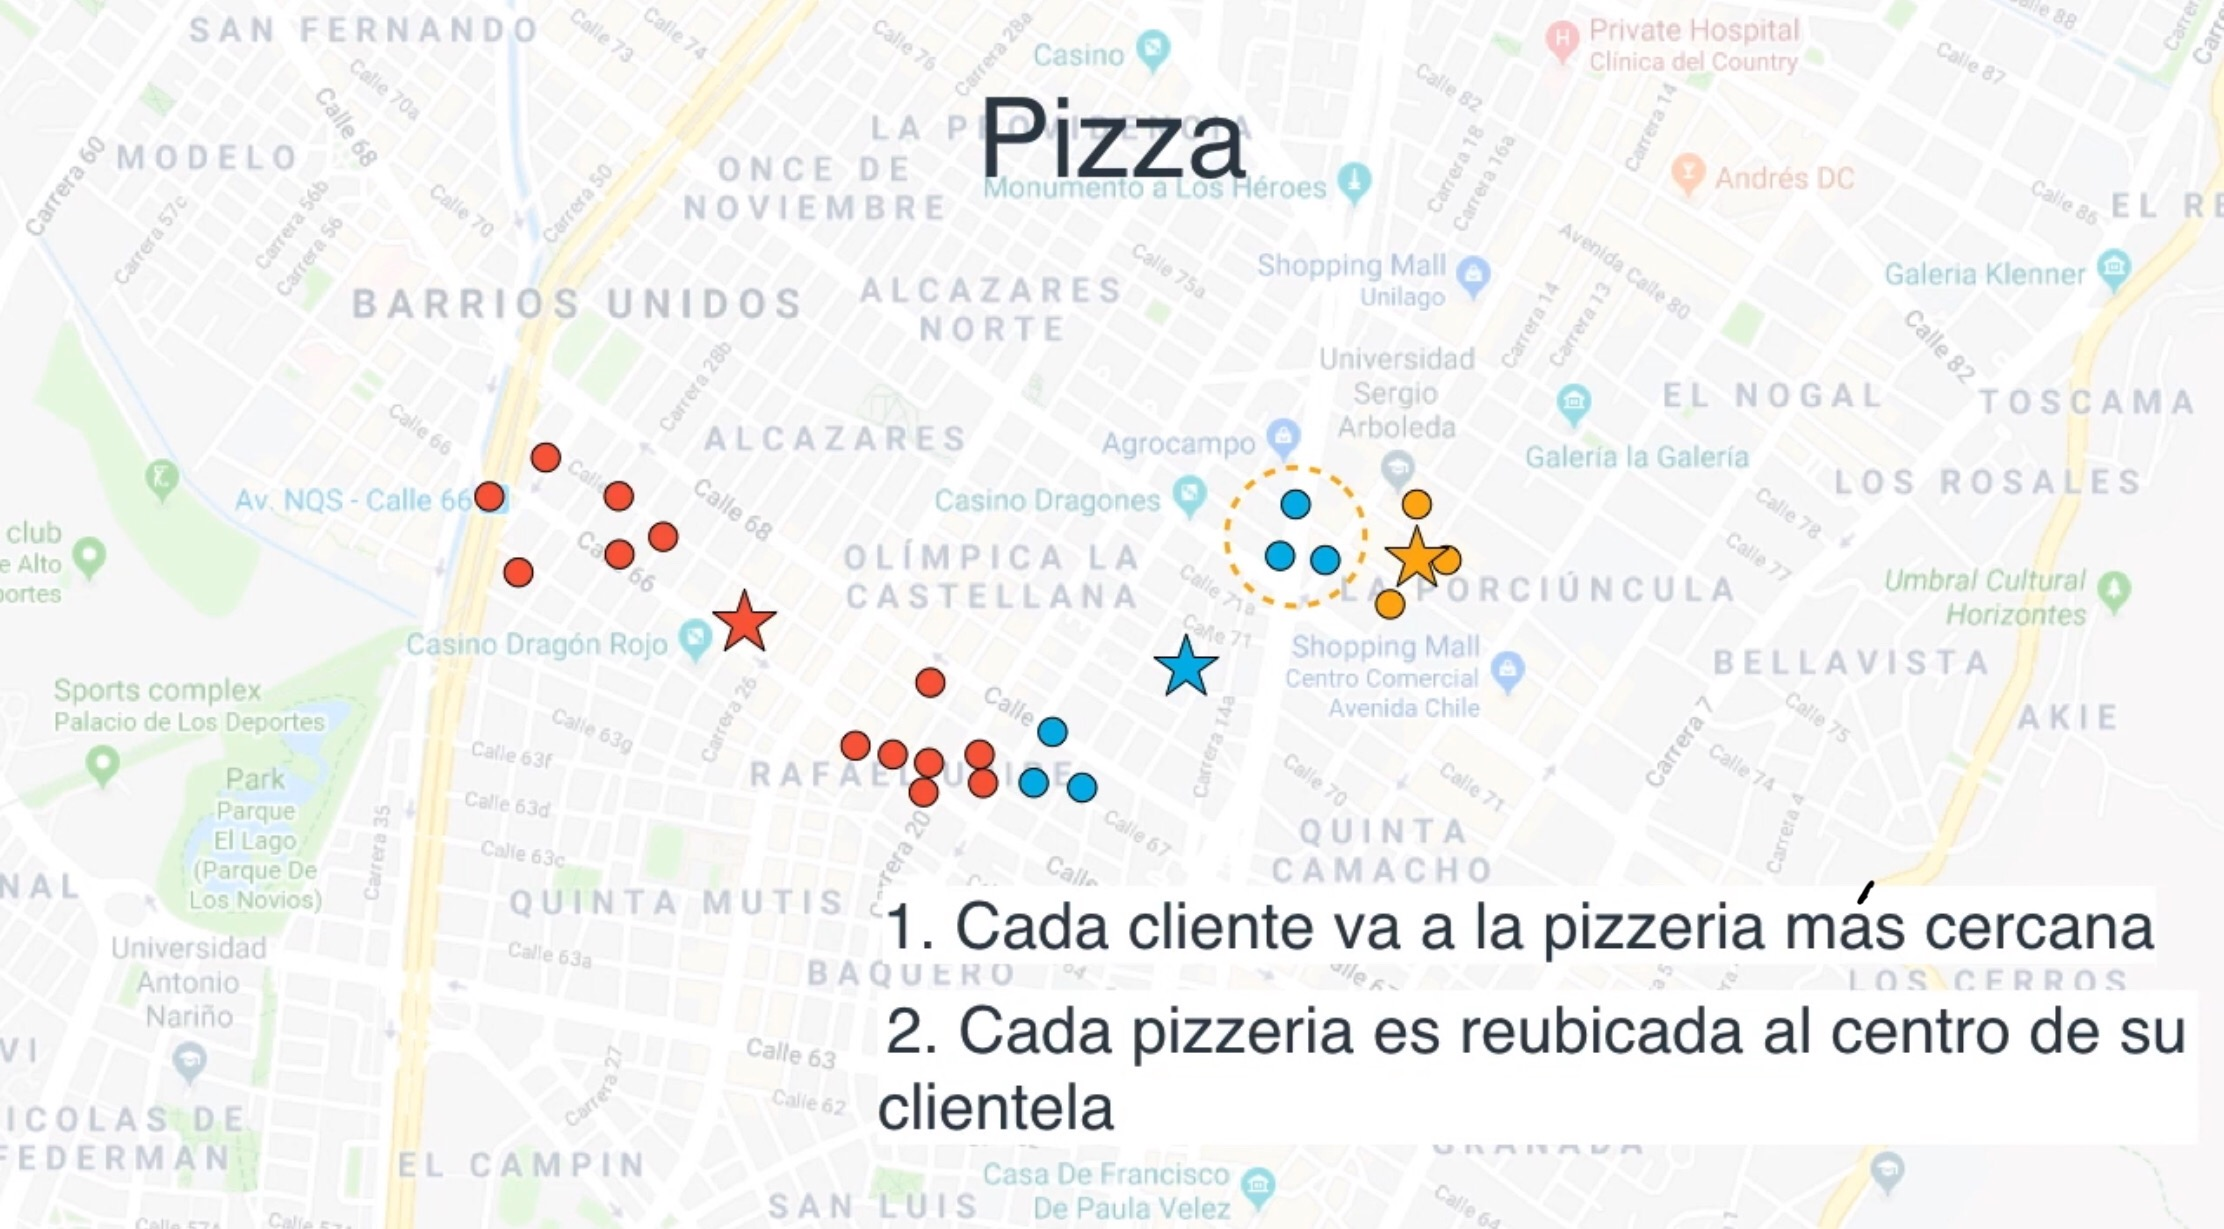
\includegraphics[width=0.9\textwidth]{Imagenes_k_means/IMG_3513.jpg}
			\caption{https://serrano.academy/espanol/}
		\end{figure}
	\end{block}
\end{frame}

\begin{frame}
	\frametitle{MÉTODOS NO SUPERVISADOS}
	\begin{block}{K Medias}	
		\begin{figure}
			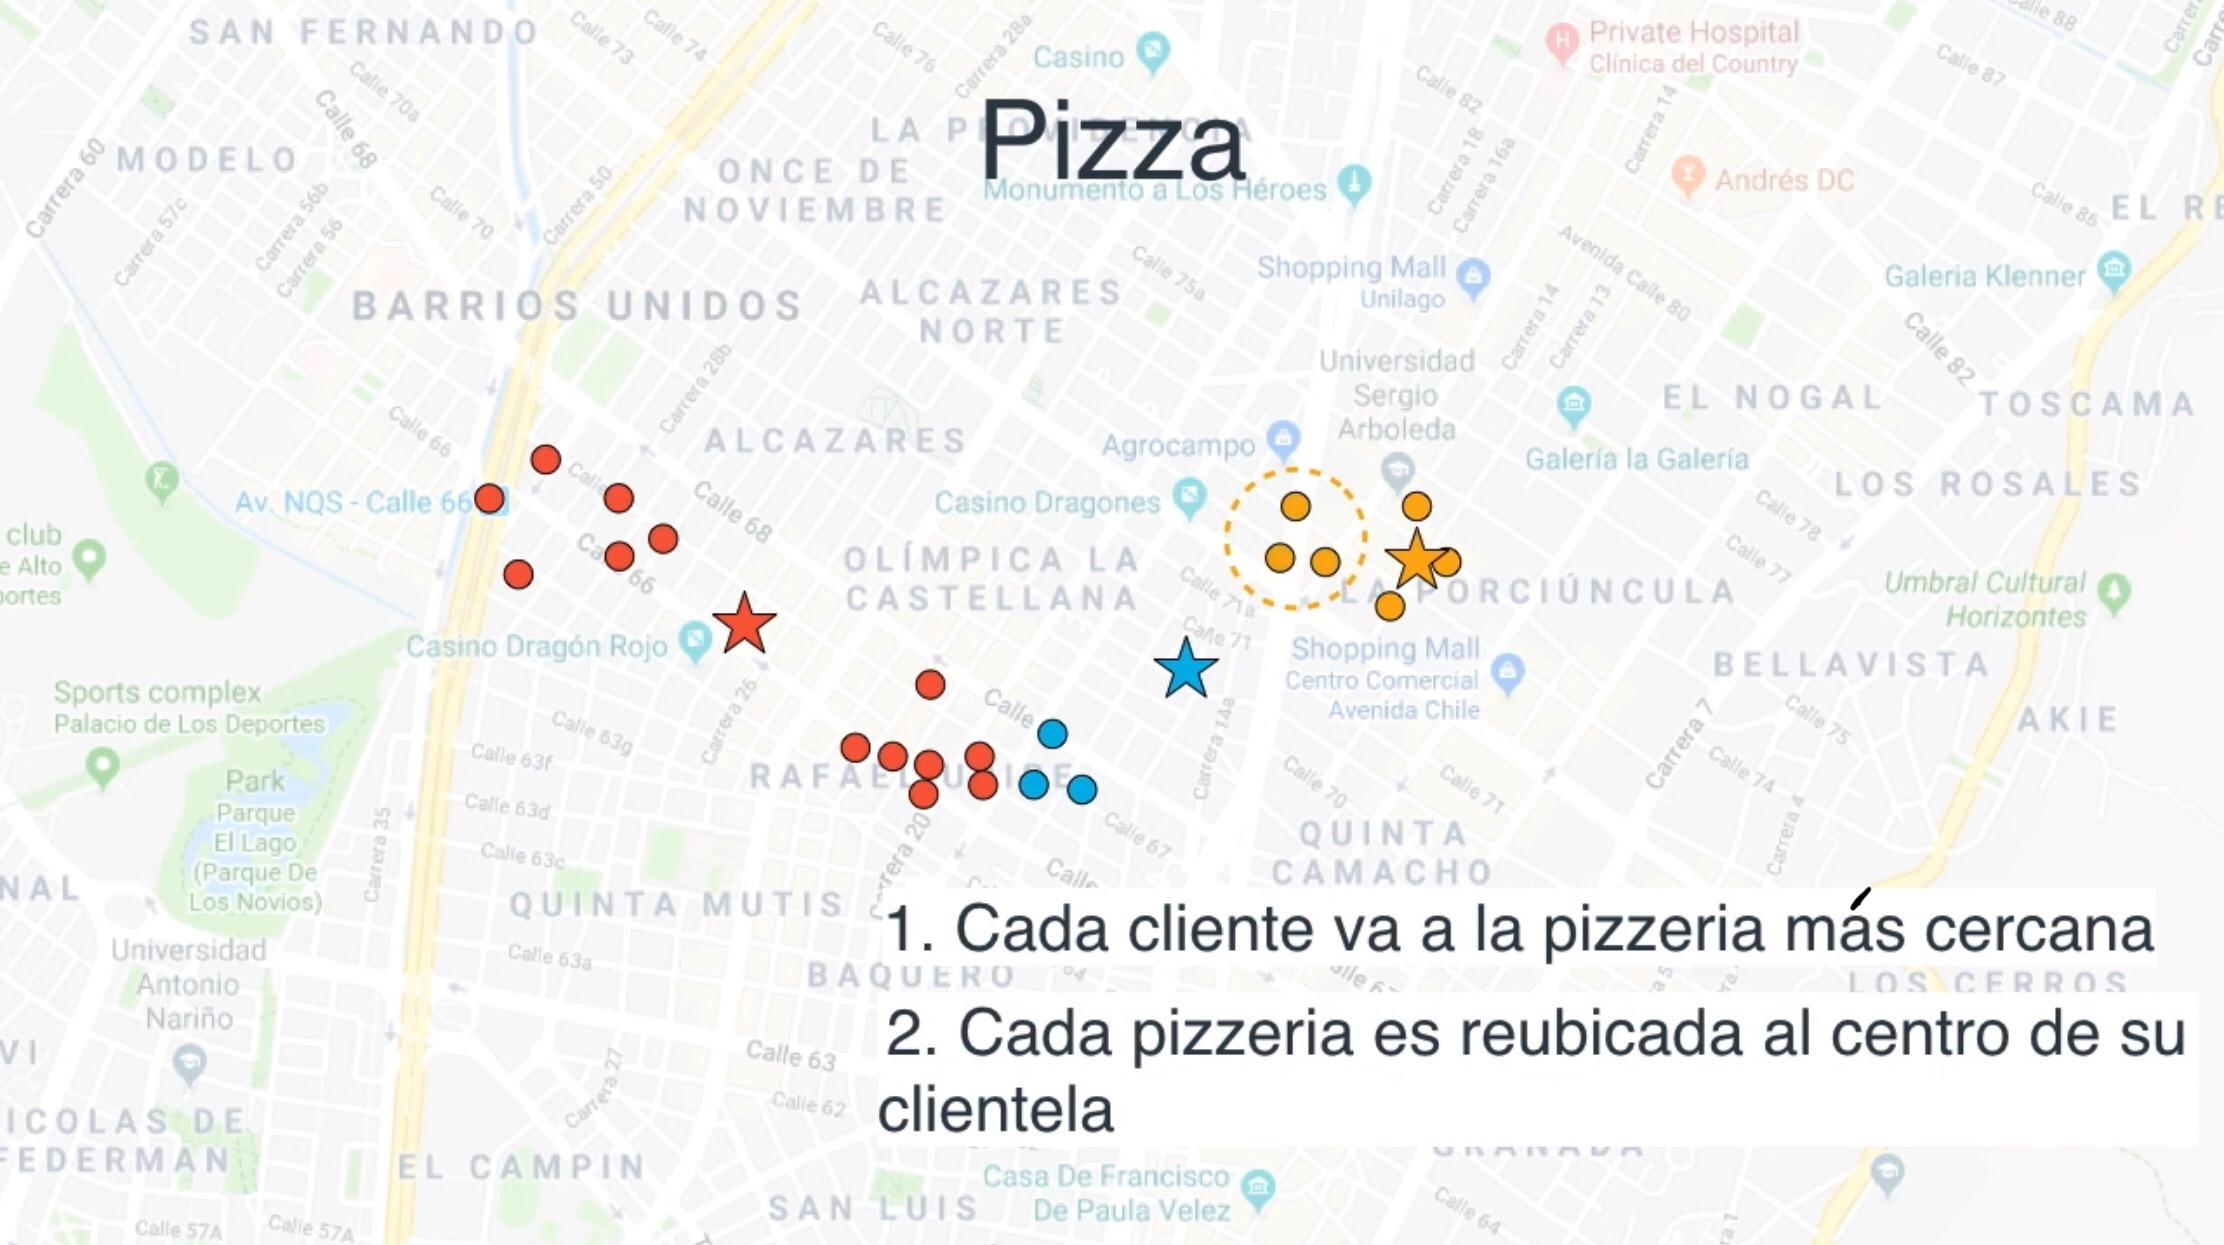
\includegraphics[width=0.9\textwidth]{Imagenes_k_means/IMG_3514.jpg}
			\caption{https://serrano.academy/espanol/}
		\end{figure}
	\end{block}
\end{frame}

\begin{frame}
	\frametitle{MÉTODOS NO SUPERVISADOS}
	\begin{block}{K Medias}	
		\begin{figure}
			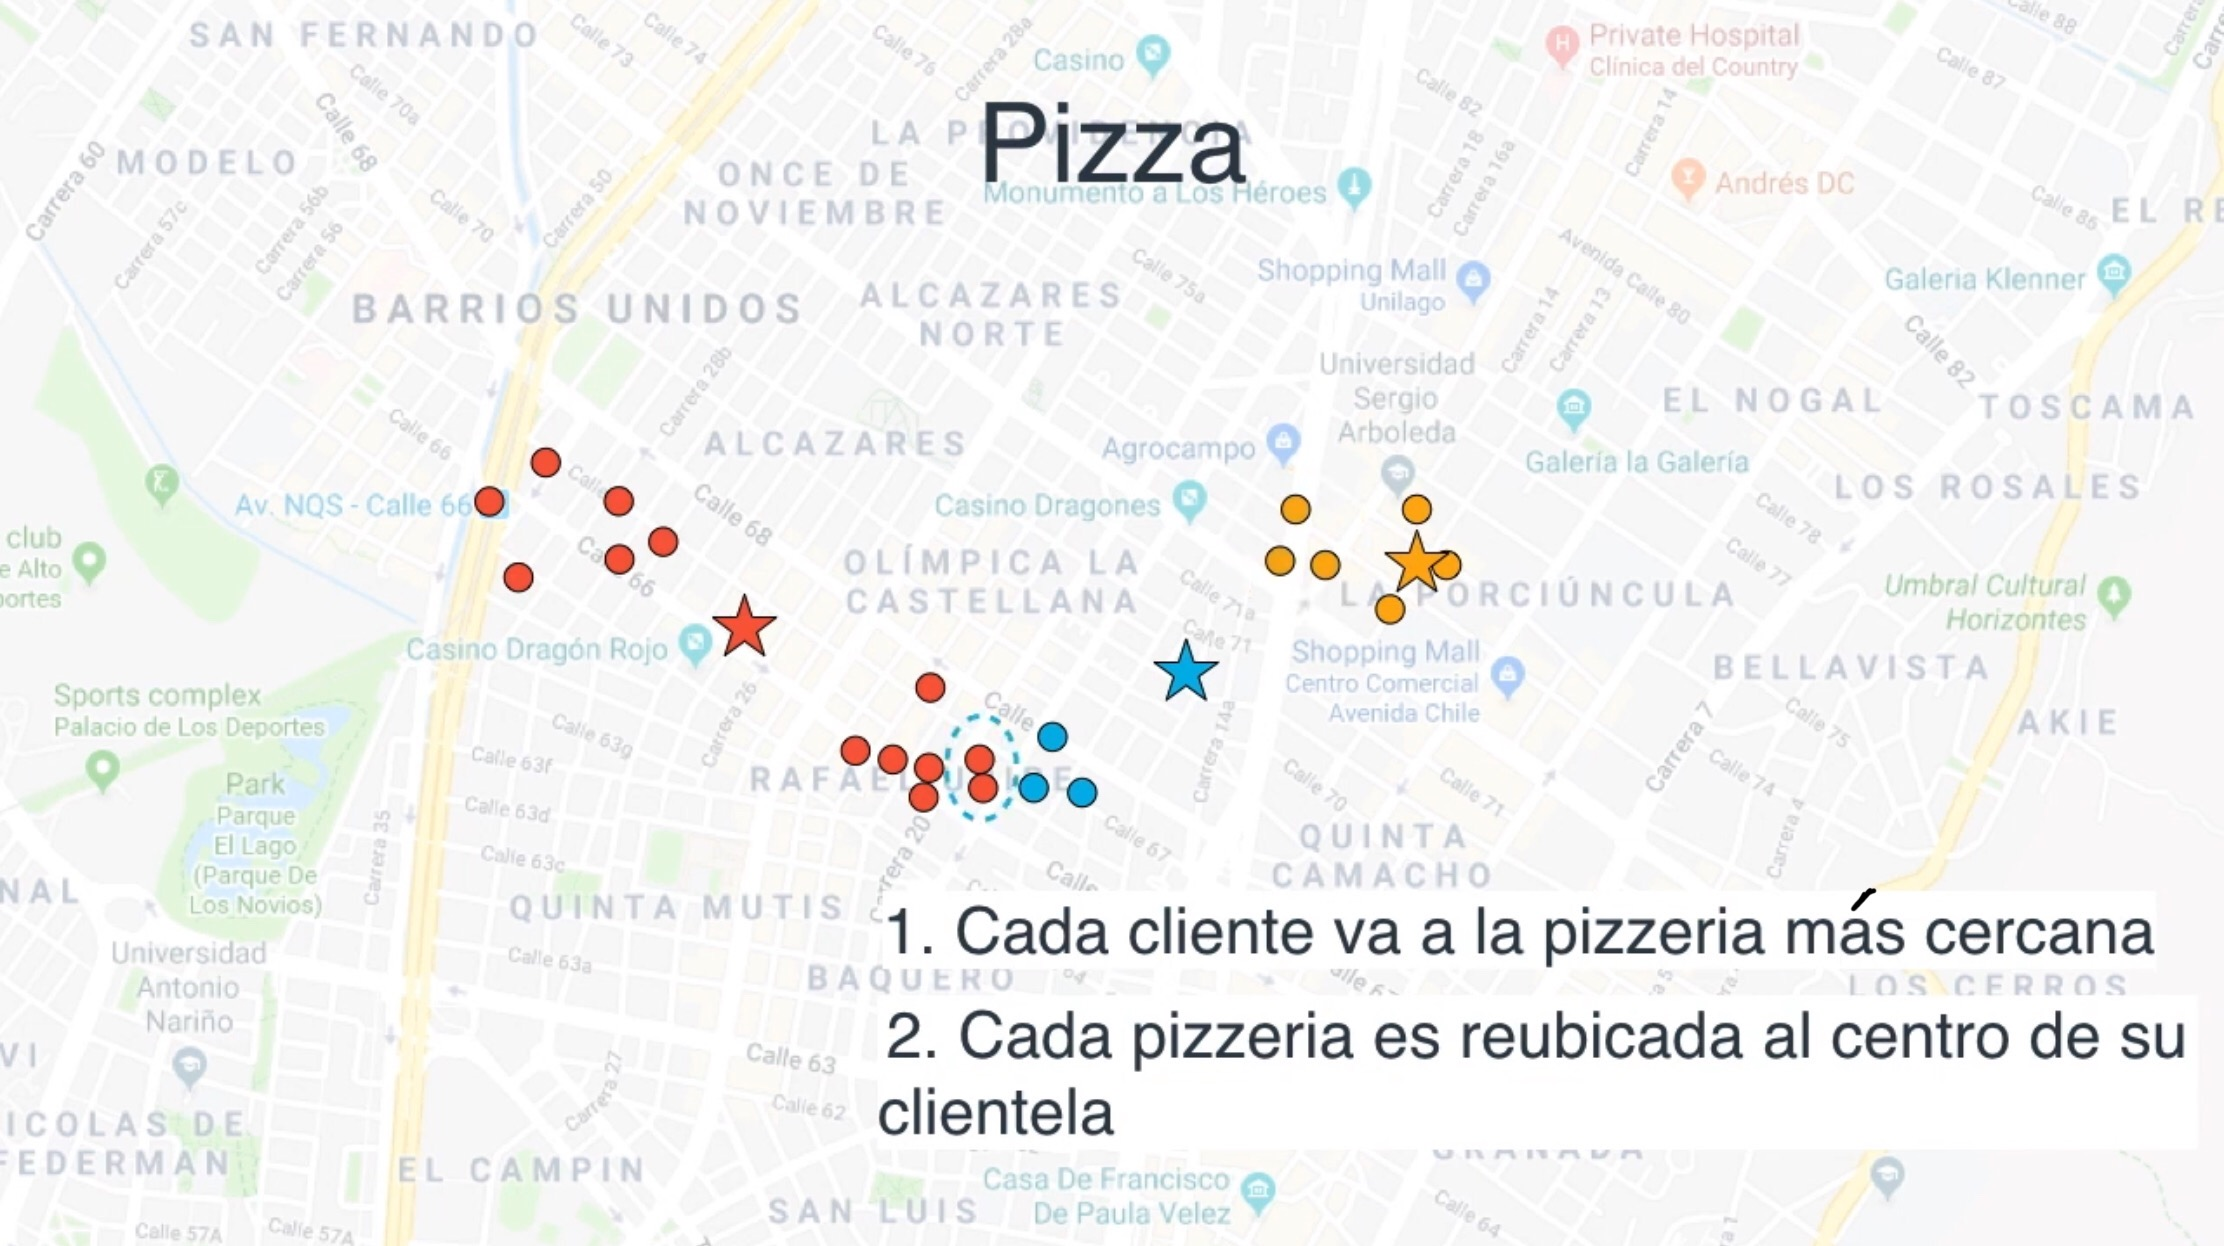
\includegraphics[width=0.9\textwidth]{Imagenes_k_means/IMG_3515.jpg}
			\caption{https://serrano.academy/espanol/}
		\end{figure}
	\end{block}
\end{frame}

\begin{frame}
	\frametitle{MÉTODOS NO SUPERVISADOS}
	\begin{block}{K Medias}	
		\begin{figure}
			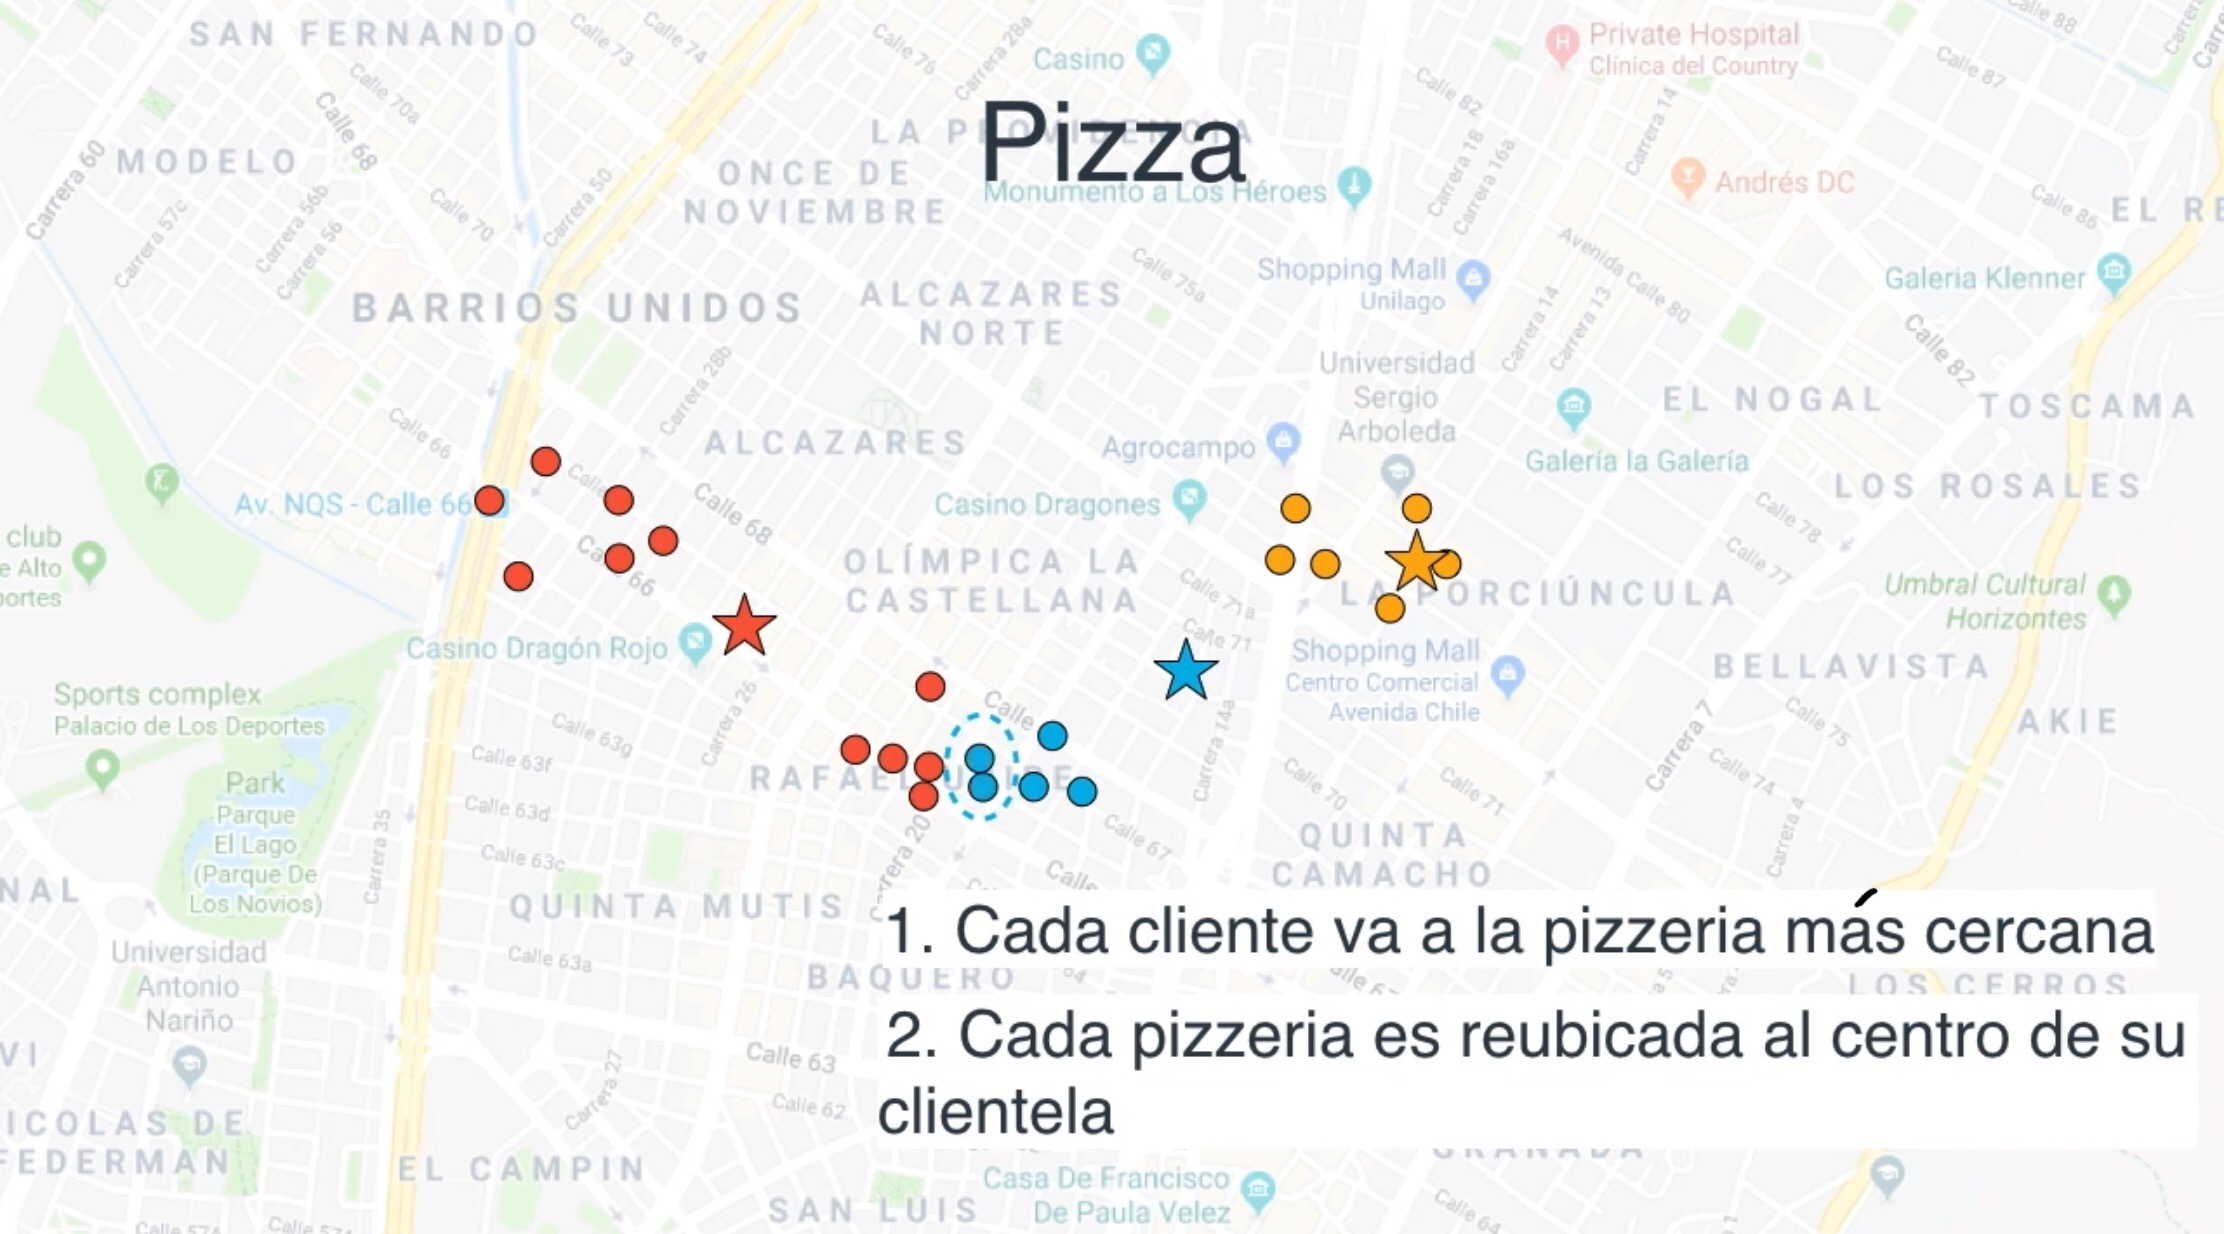
\includegraphics[width=0.9\textwidth]{Imagenes_k_means/IMG_3516.jpg}
			\caption{https://serrano.academy/espanol/}
		\end{figure}
	\end{block}
\end{frame}

\begin{frame}
	\frametitle{MÉTODOS NO SUPERVISADOS}
	\begin{block}{K Medias}	
		\begin{figure}
			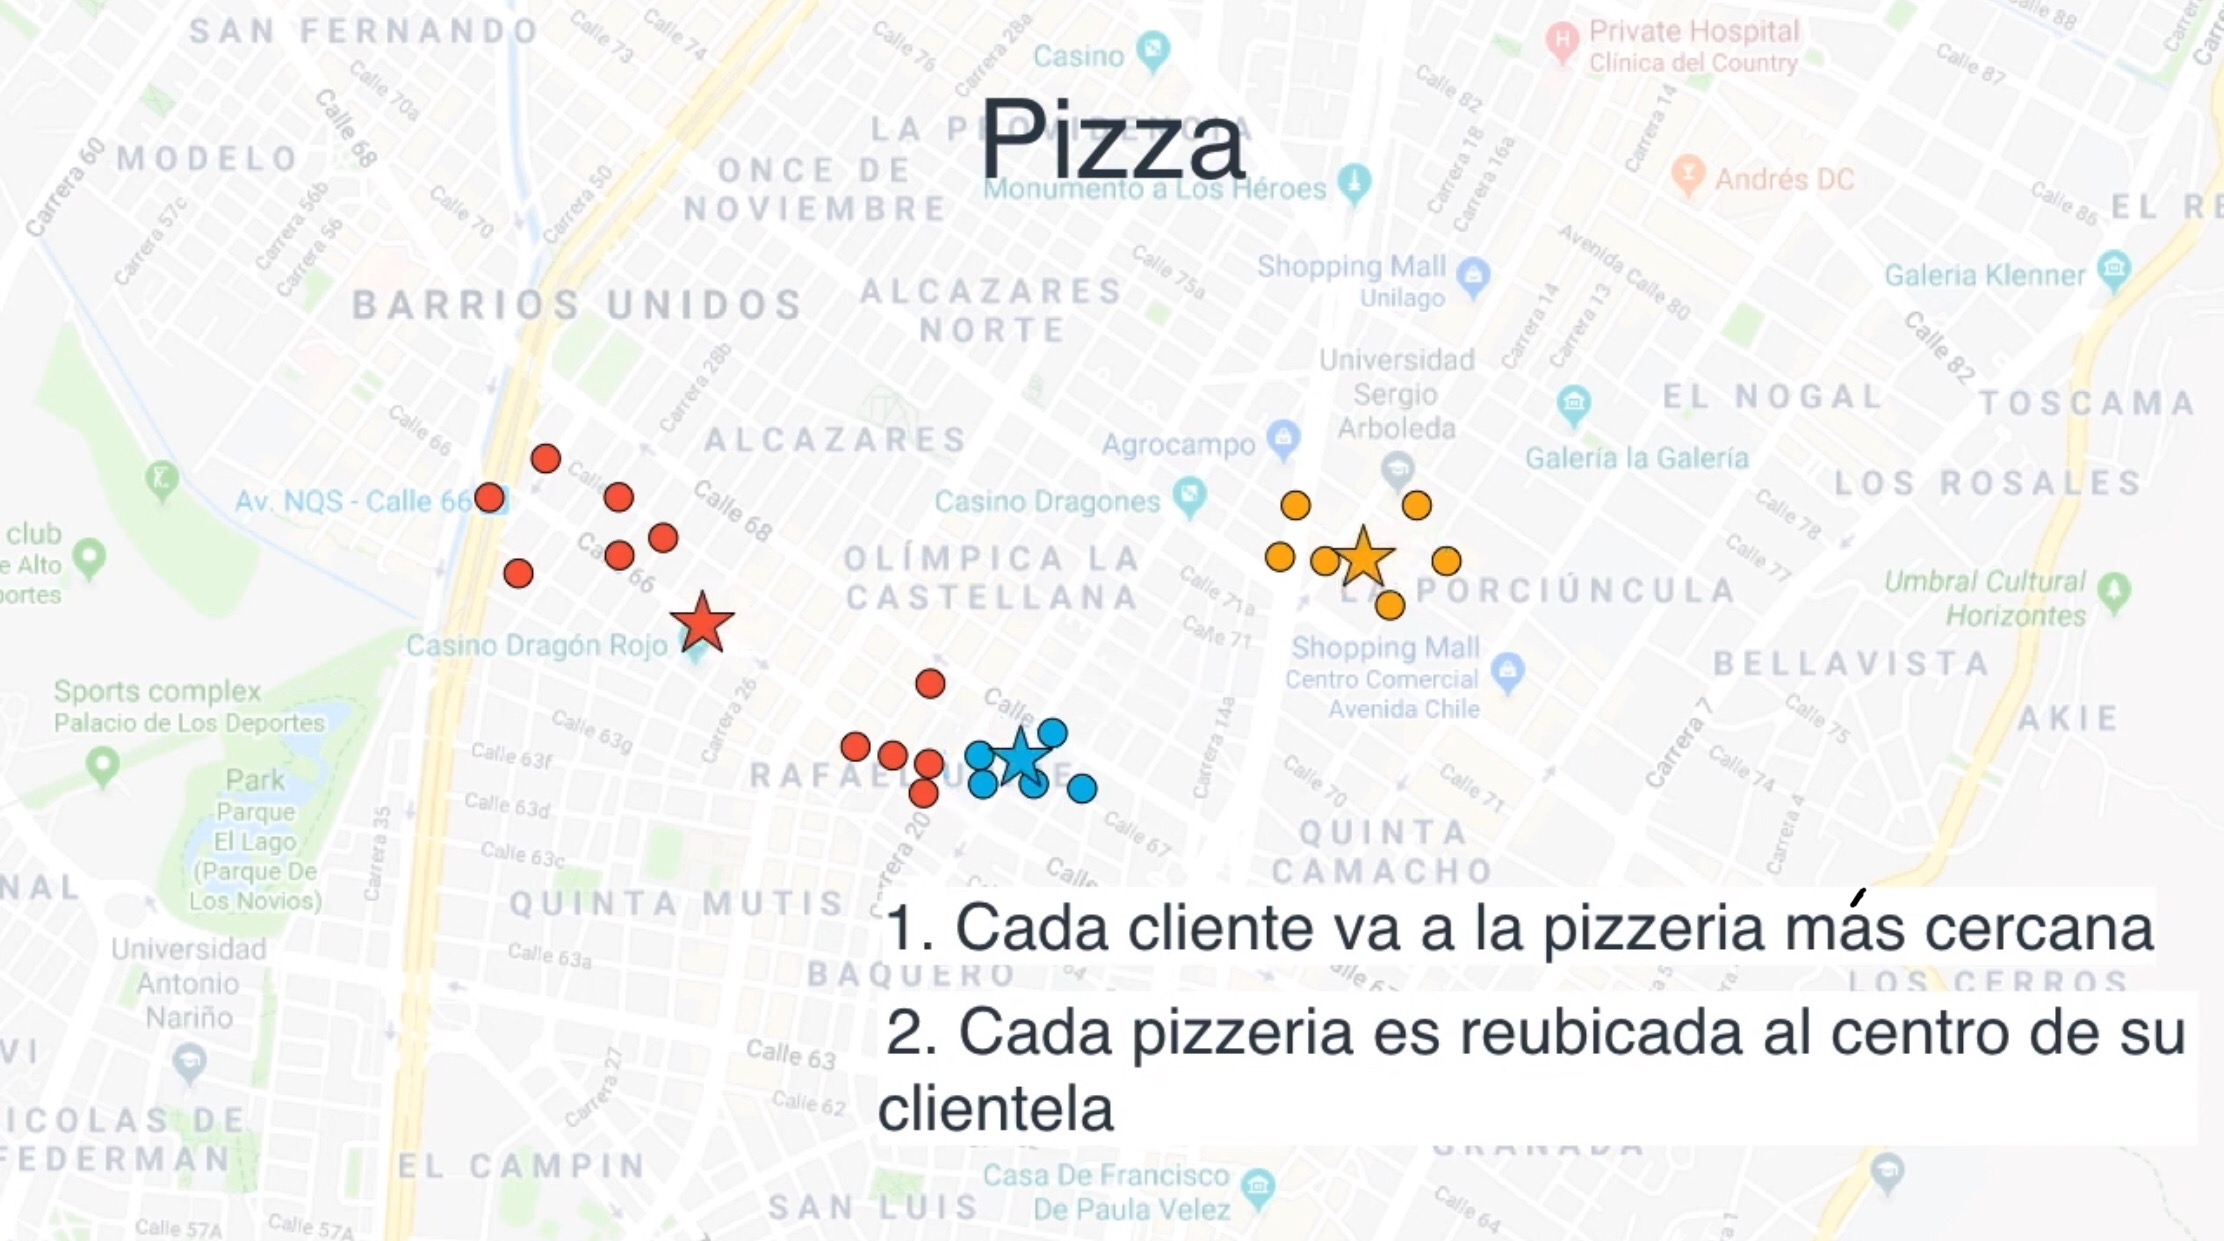
\includegraphics[width=0.9\textwidth]{Imagenes_k_means/IMG_3517.jpg}
			\caption{https://serrano.academy/espanol/}
		\end{figure}
	\end{block}
\end{frame}


\begin{frame}
	\frametitle{MÉTODOS NO SUPERVISADOS}
	\begin{block}{K Medias}	
		\begin{figure}
			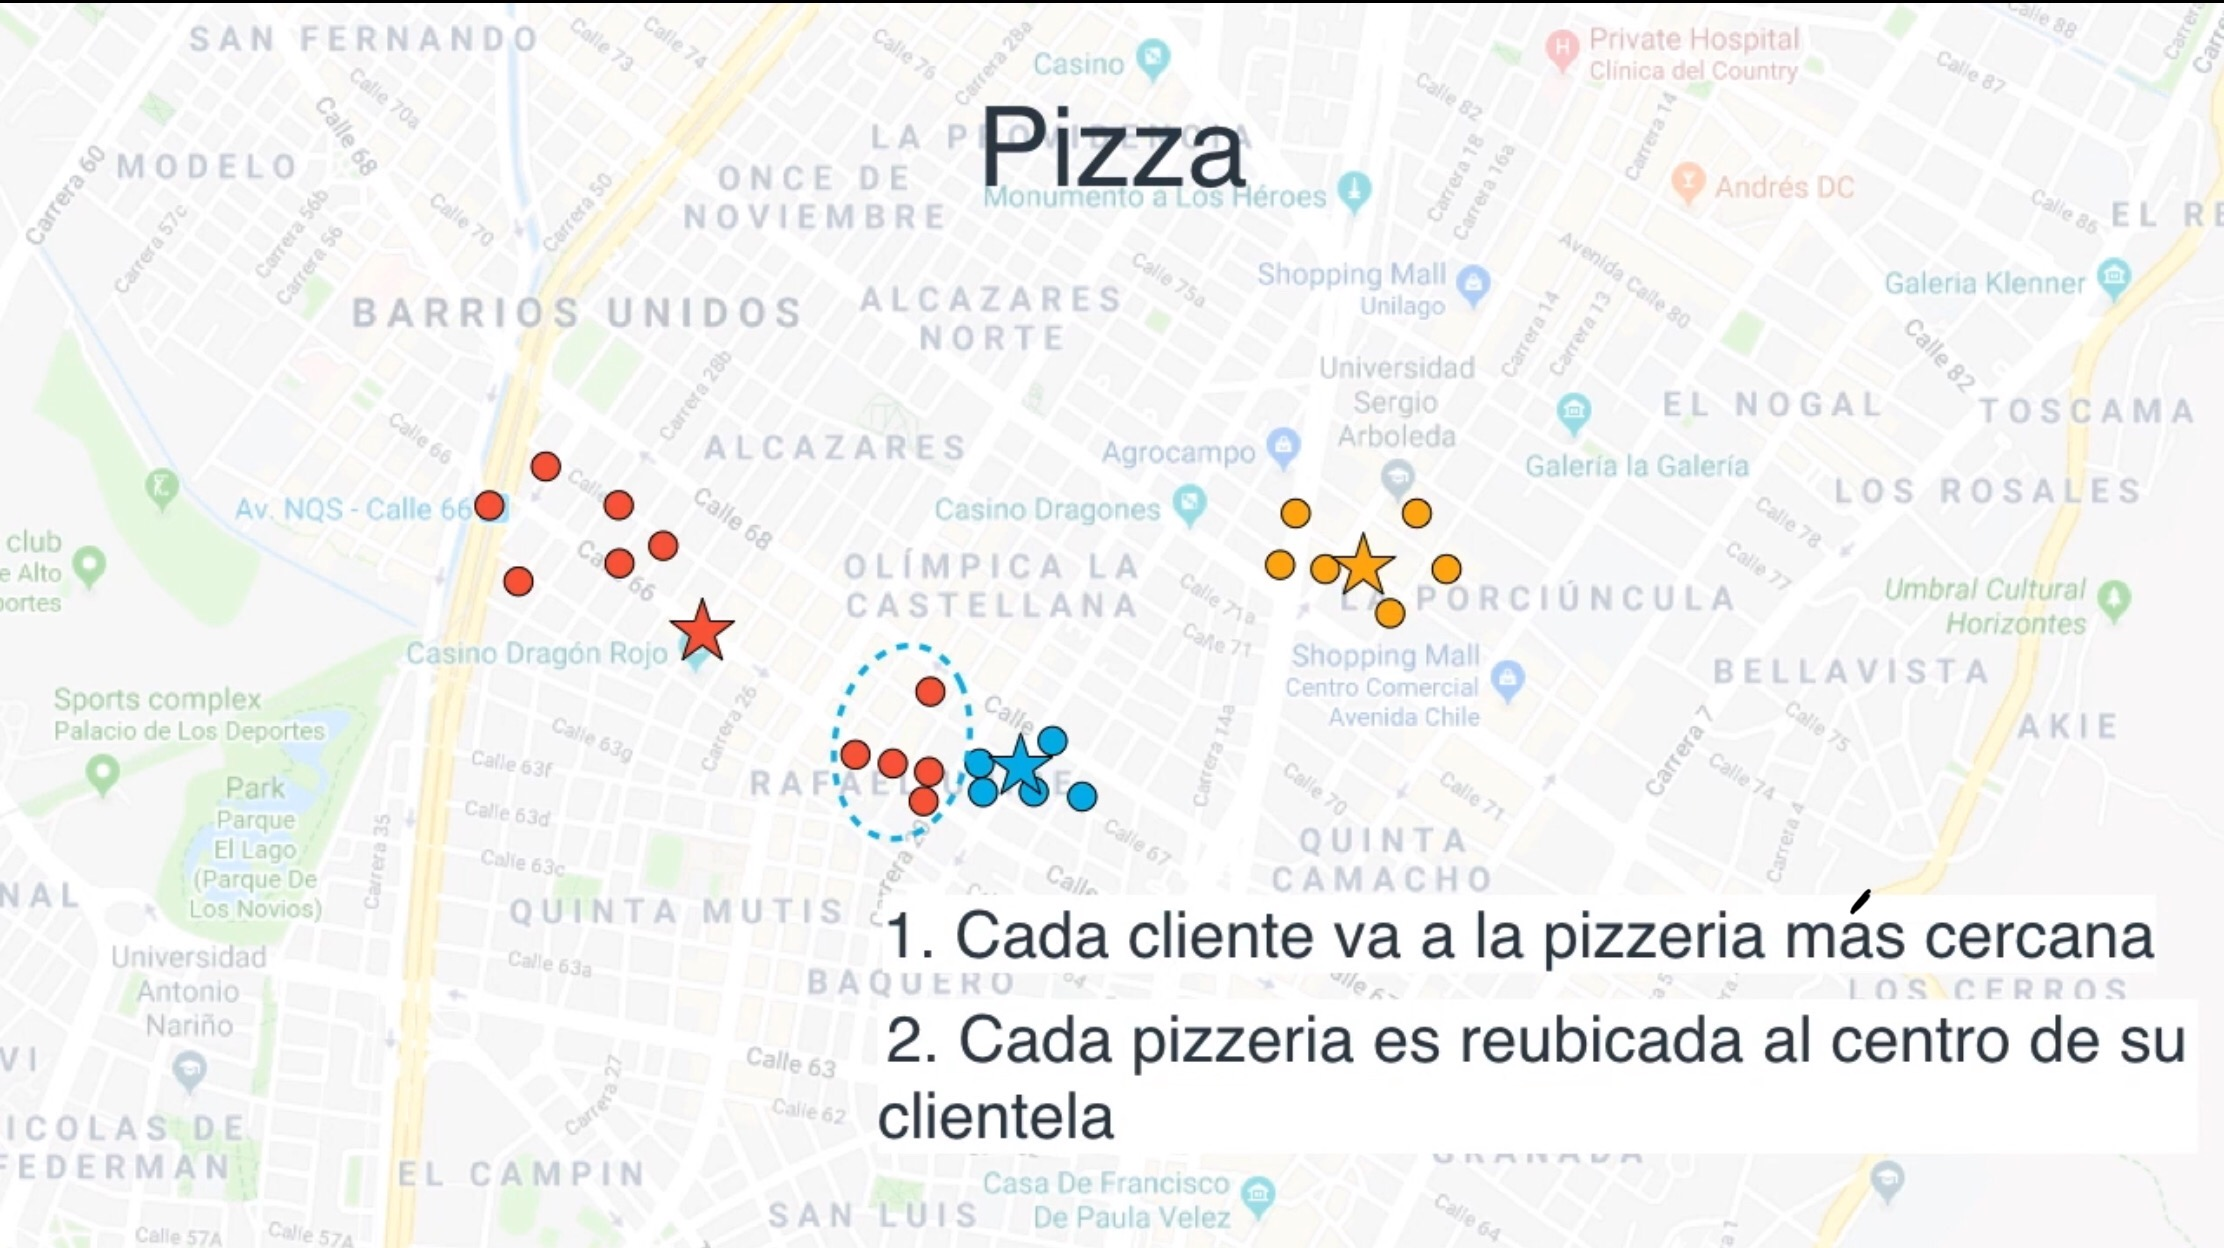
\includegraphics[width=0.9\textwidth]{Imagenes_k_means/IMG_3518.jpg}
			\caption{https://serrano.academy/espanol/}
		\end{figure}
	\end{block}
\end{frame}

\begin{frame}
	\frametitle{MÉTODOS NO SUPERVISADOS}
	\begin{block}{K Medias}	
		\begin{figure}
			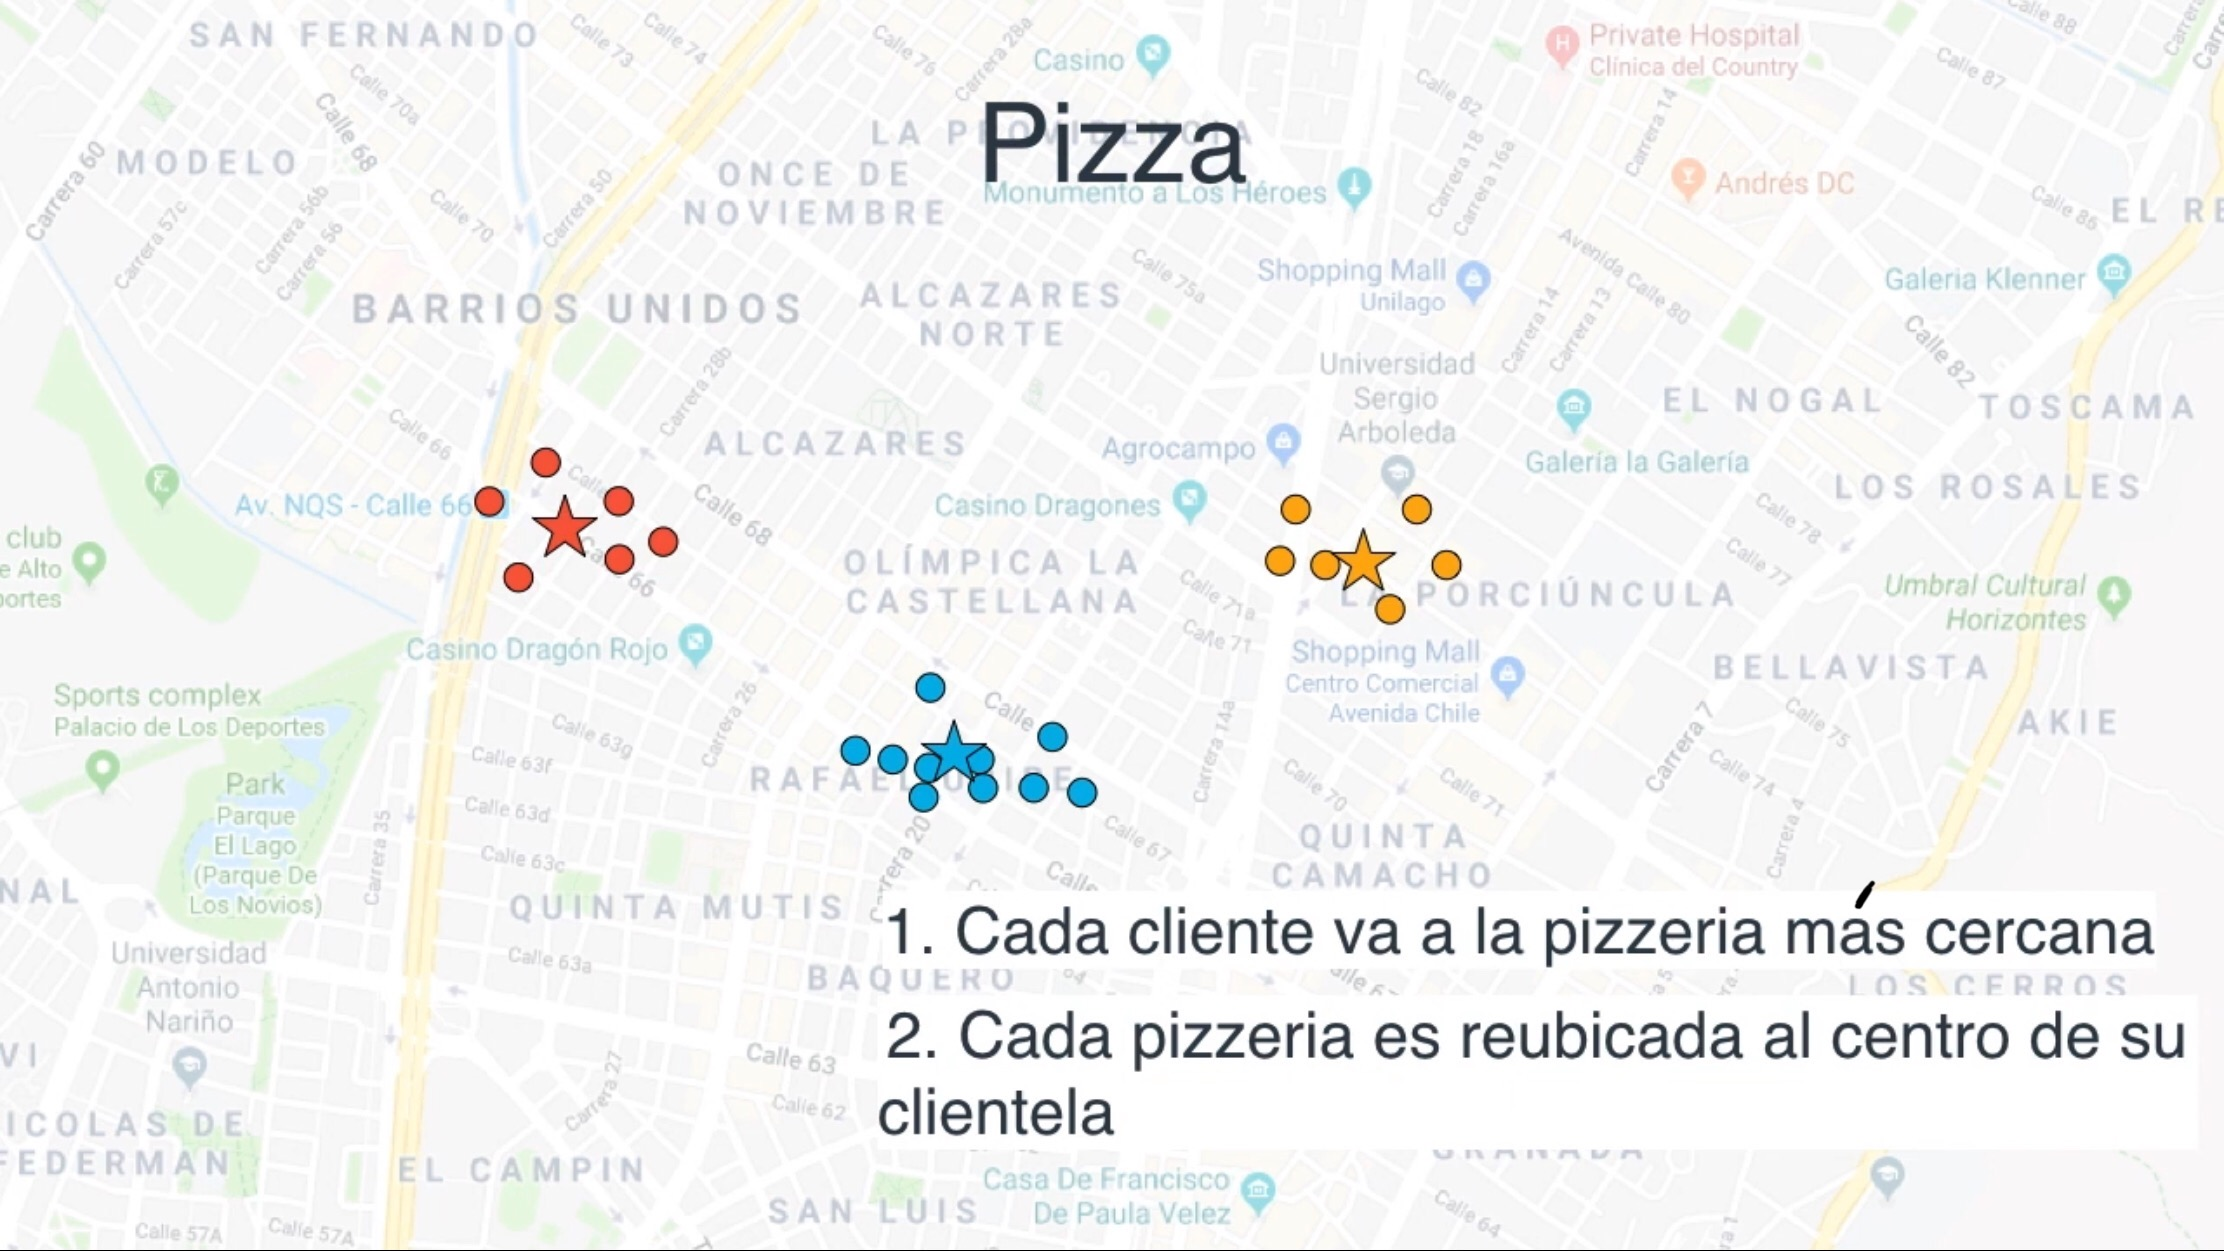
\includegraphics[width=0.9\textwidth]{Imagenes_k_means/IMG_3519.jpg}
			\caption{https://serrano.academy/espanol/}
		\end{figure}
	\end{block}
\end{frame}

\begin{frame}
	\frametitle{MÉTODOS NO SUPERVISADOS}
	\begin{block}{K Medias}	
	\textbf{	¿Cómo sabemos cuántos grupos usar?}
	\end{block}
\end{frame}

\begin{frame}
	\frametitle{MÉTODOS NO SUPERVISADOS}
	\begin{block}{K Medias}	
		\begin{figure}
			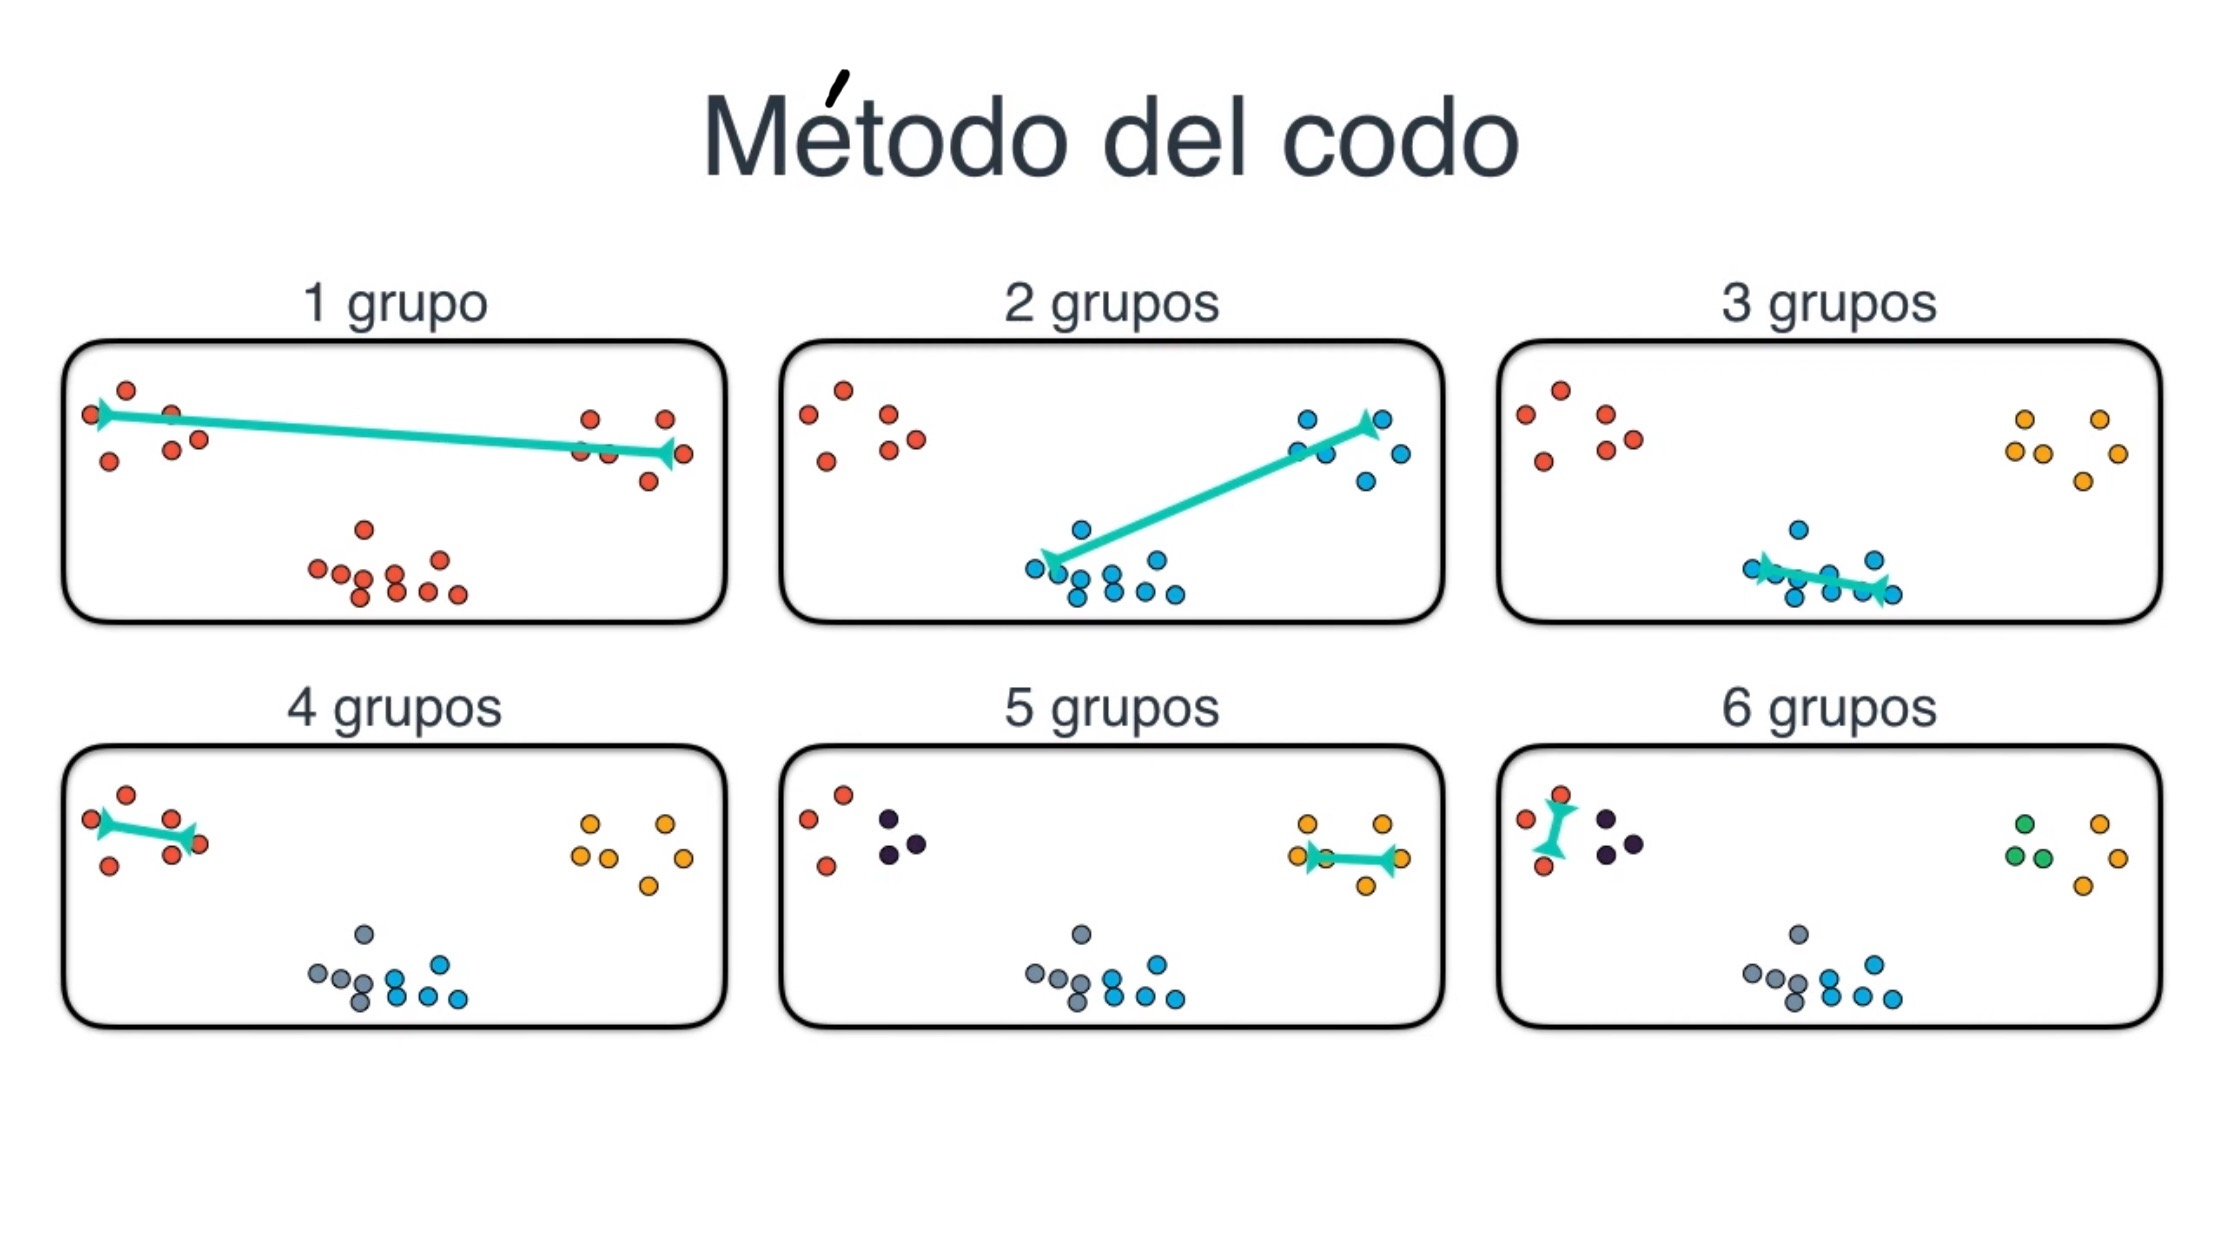
\includegraphics[width=0.9\textwidth]{Imagenes_k_means/IMG_3521.jpg}
			\caption{https://serrano.academy/espanol/}
		\end{figure}
	\end{block}
\end{frame}

\begin{frame}
	\frametitle{MÉTODOS NO SUPERVISADOS}
	\begin{block}{K Medias}	
		\begin{figure}
			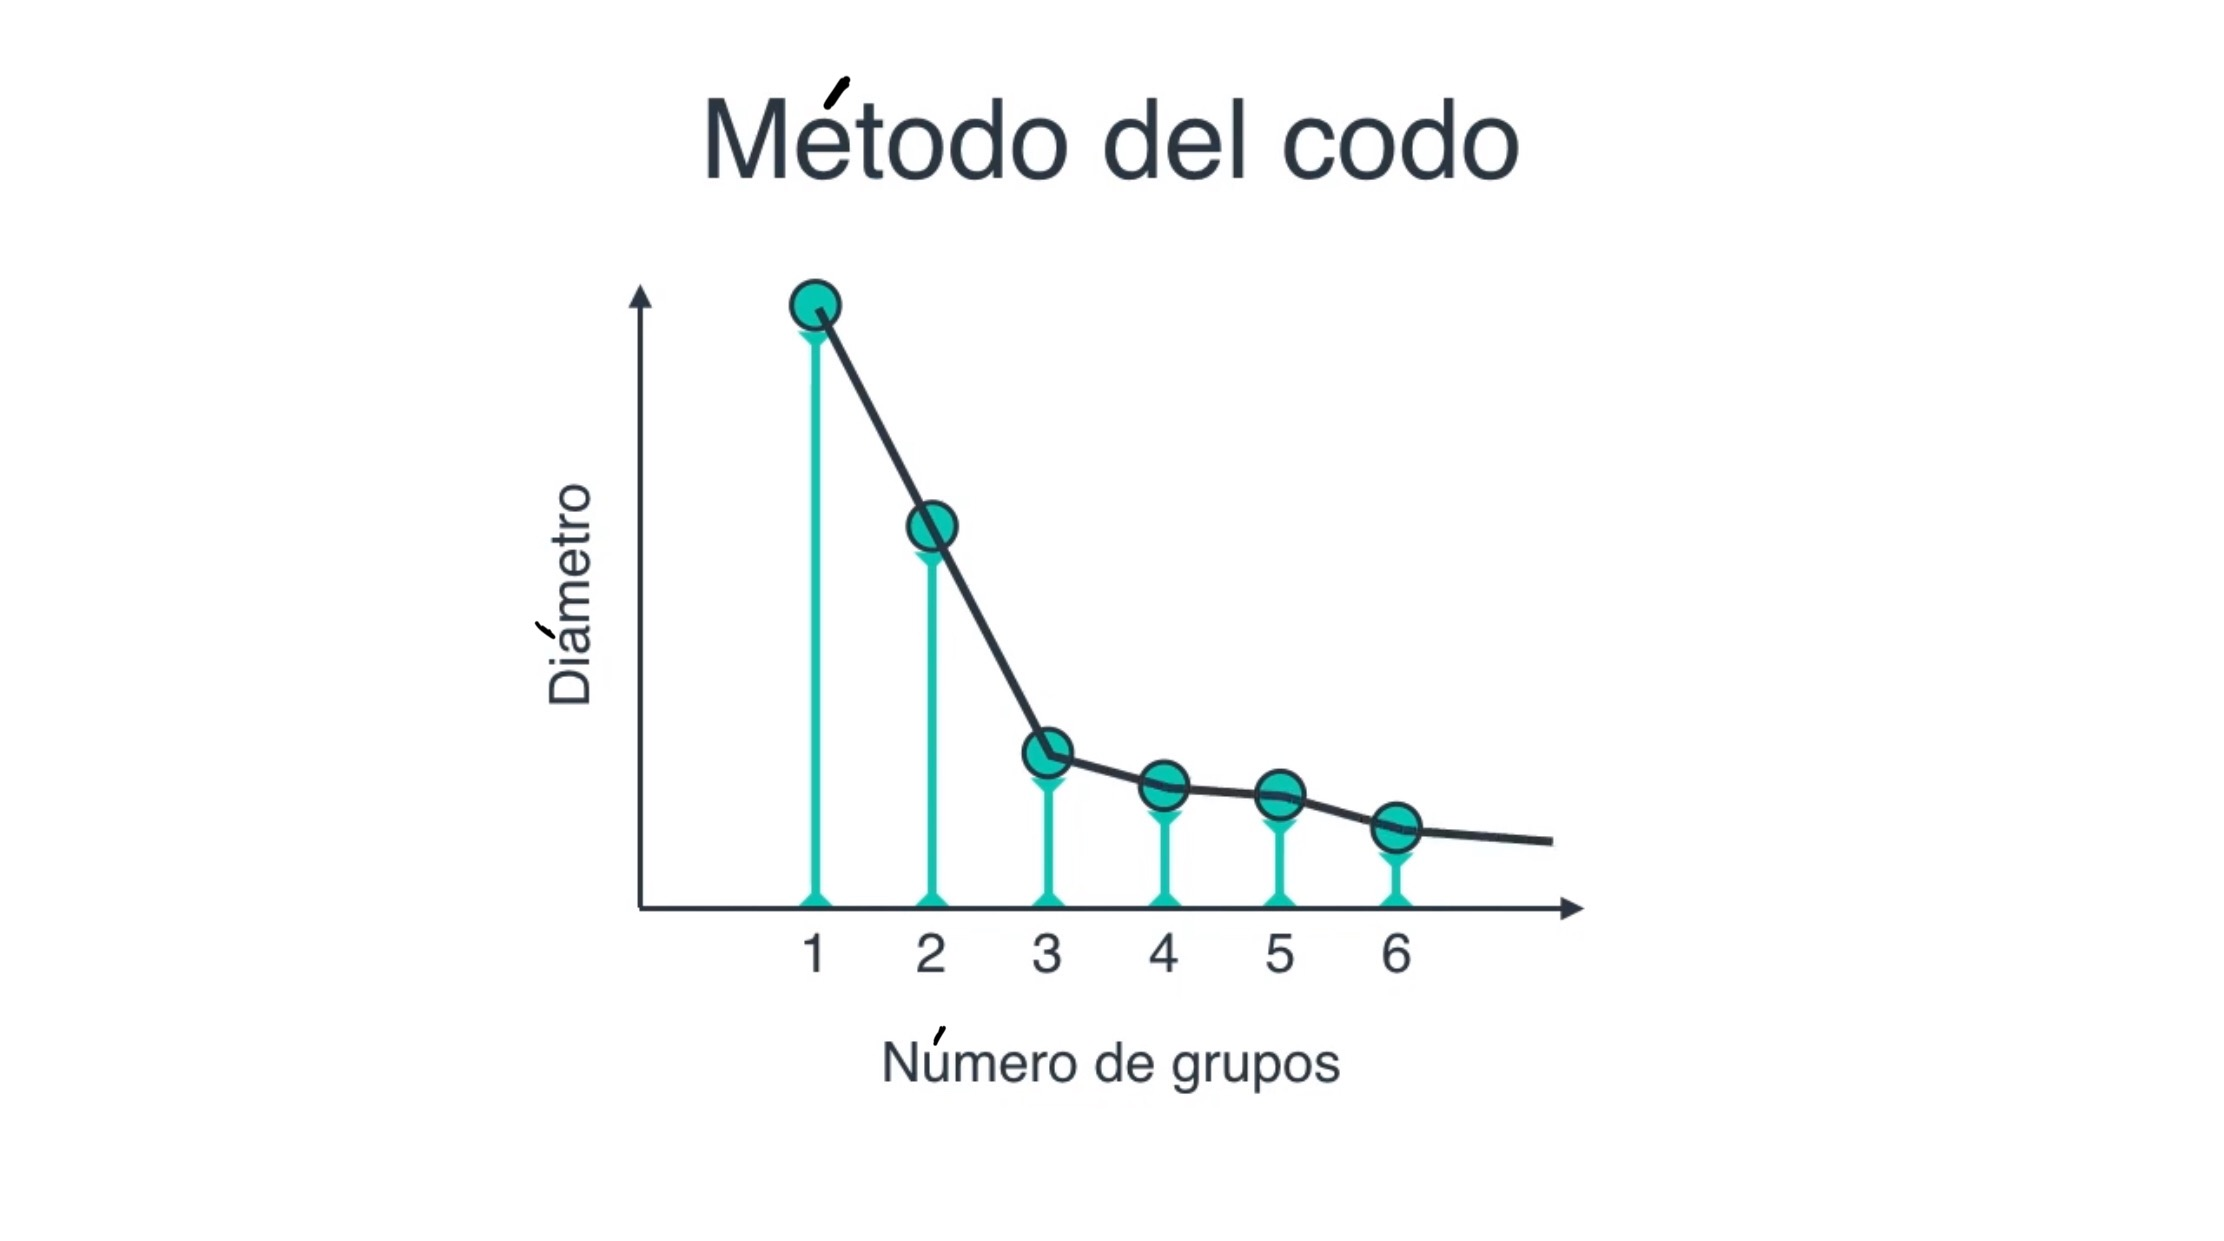
\includegraphics[width=0.9\textwidth]{Imagenes_k_means/IMG_3523.jpg}
			\caption{https://serrano.academy/espanol/}
		\end{figure}
	\end{block}
\end{frame}

\begin{frame}
	\frametitle{MÉTODOS NO SUPERVISADOS}
	\begin{block}{K Medias}	
		\begin{figure}
			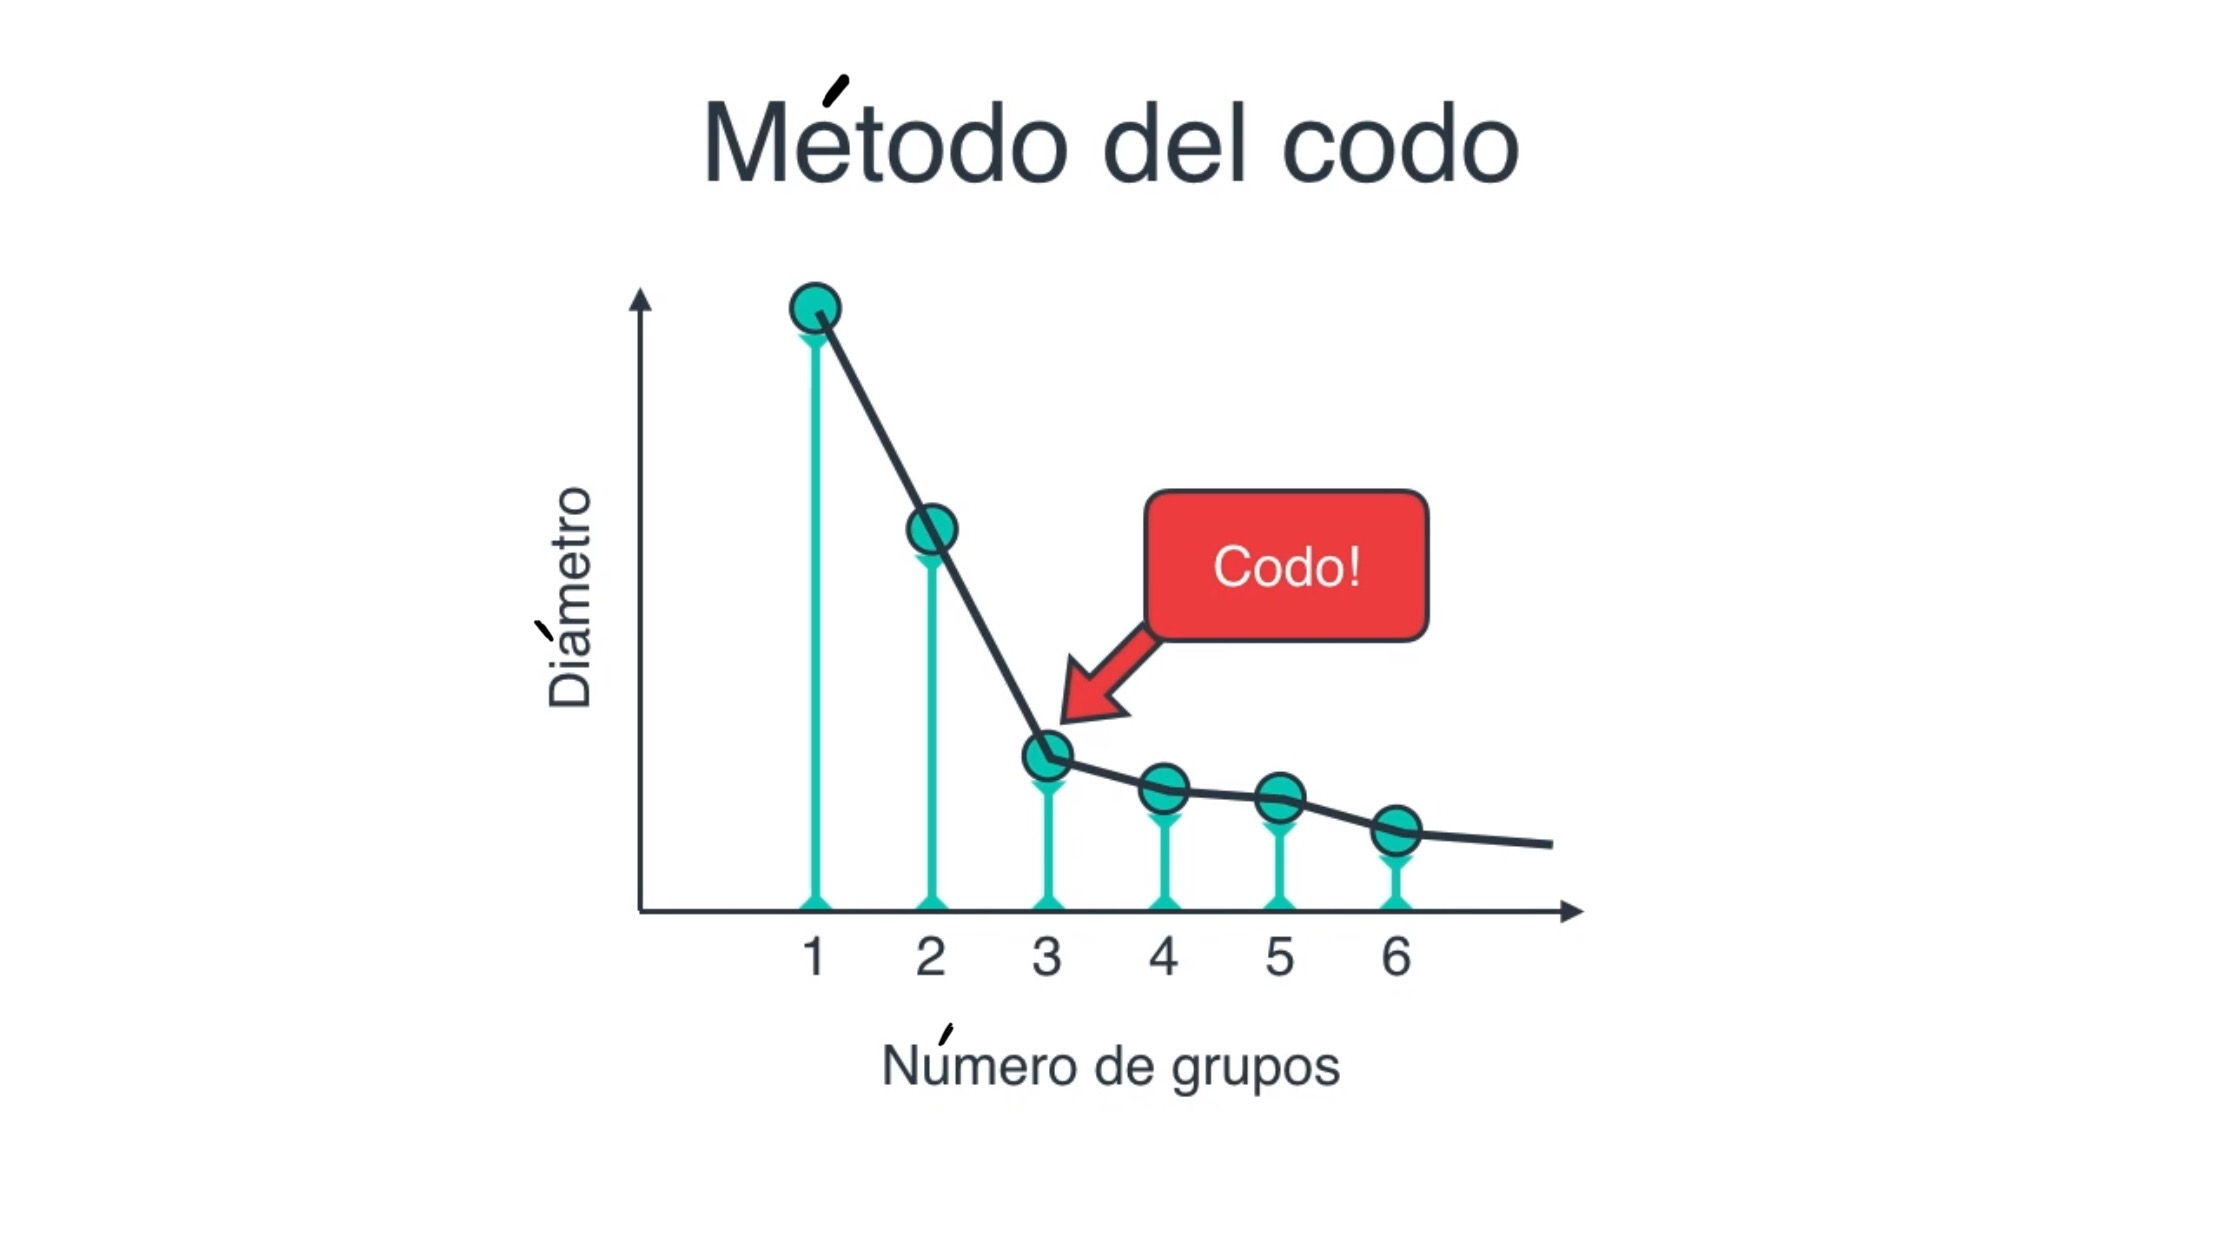
\includegraphics[width=0.9\textwidth]{Imagenes_k_means/IMG_3524.jpg}
			\caption{https://serrano.academy/espanol/}
		\end{figure}
	\end{block}
\end{frame}


\section{REDUCCIÓN DE DIMENSIONALIDAD}

\begin{frame}
	\frametitle{MODELOS DE APRENDIZAJE DE MÁQUINA}
	\begin{block}{}	
		\center
		\textbf{ANÁLISIS DE COMPONENTES PRINCIPALES}
	\end{block}
\end{frame}

\begin{frame}
	\frametitle{REDUCCIÓN DE DIMENSIONALIDAD}
	\begin{block}{Análisis de Componentes Principales}	
		\begin{figure}
			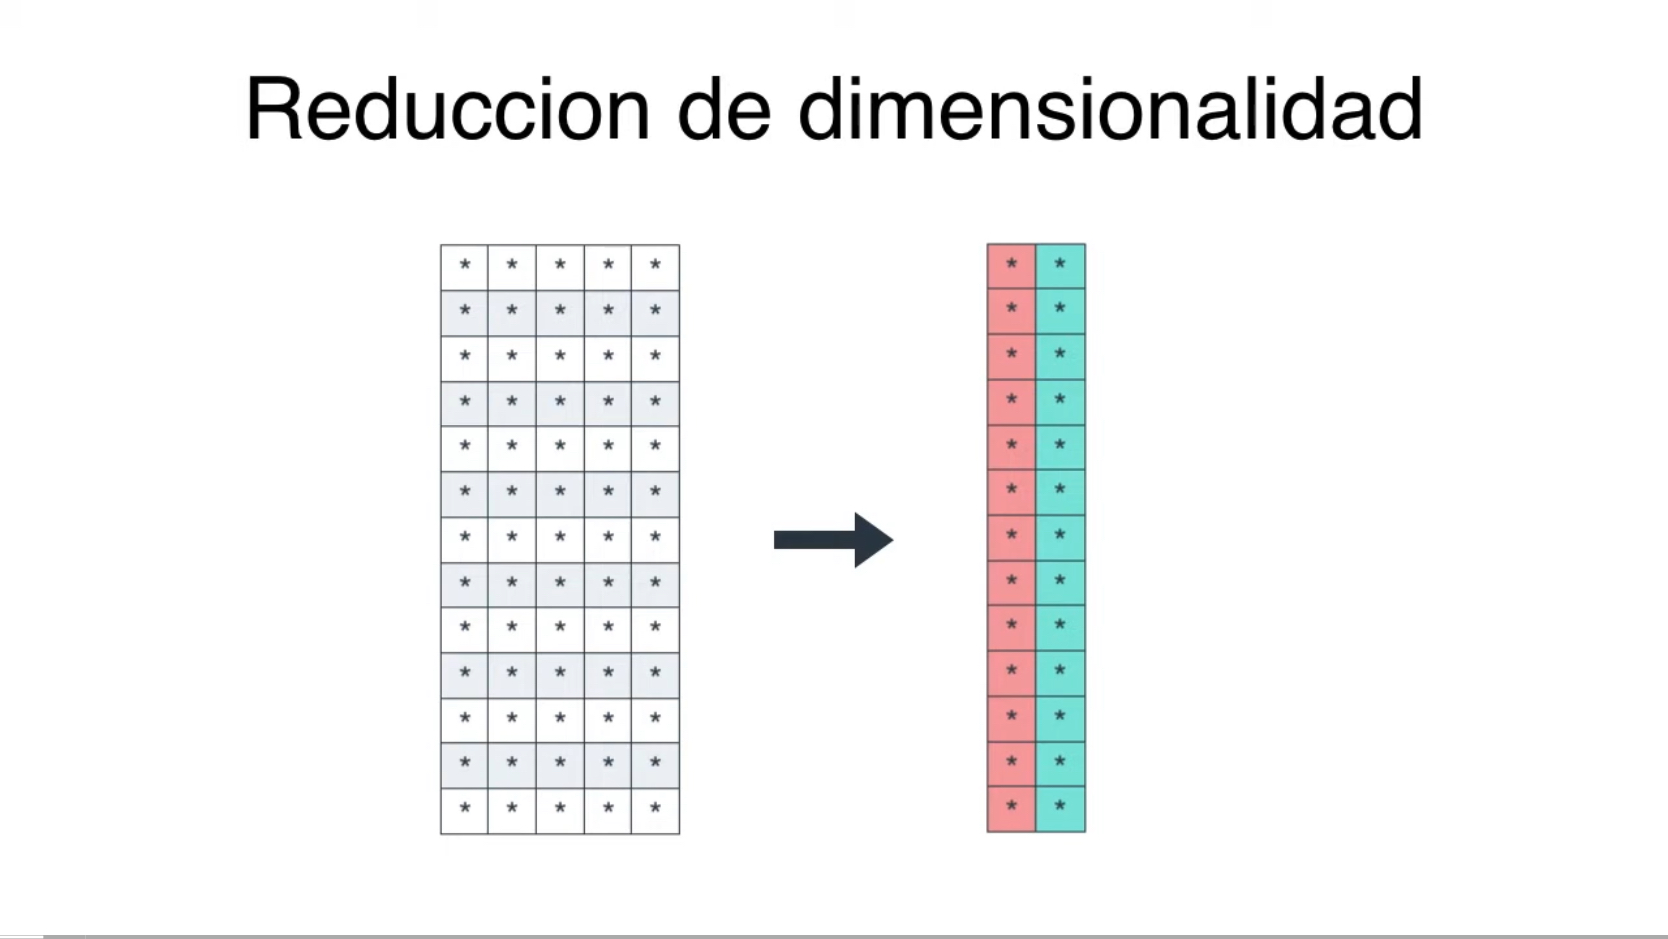
\includegraphics[width=0.9\textwidth]{PCA/IMG_3525.jpg}
			\caption{https://serrano.academy/espanol/}
		\end{figure}
	\end{block}
\end{frame}

\begin{frame}
\frametitle{REDUCCIÓN DE DIMENSIONALIDAD}
\begin{block}{Análisis de Componentes Principales}	
	\begin{figure}
		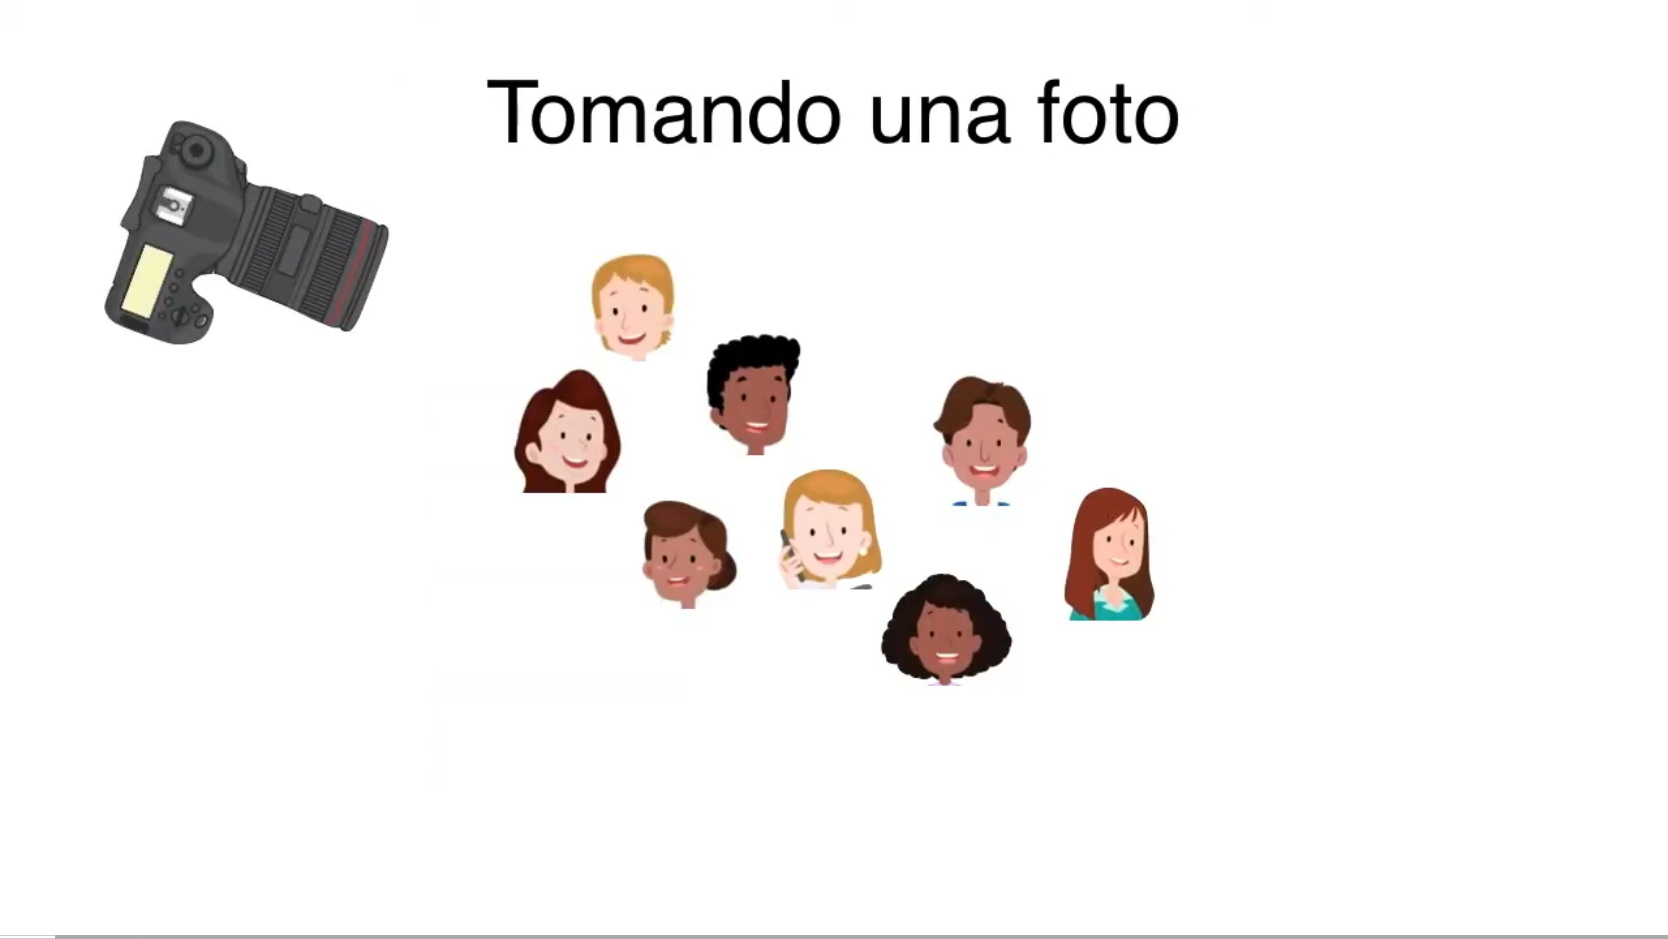
\includegraphics[width=0.9\textwidth]{PCA/IMG_3526.jpg}
		\caption{https://serrano.academy/espanol/}
	\end{figure}
\end{block}
\end{frame}

\begin{frame}
\frametitle{REDUCCIÓN DE DIMENSIONALIDAD}
\begin{block}{Análisis de Componentes Principales}	
	\begin{figure}
		\includegraphics[width=0.9\textwidth]{PCA/IMG_3527.jpg}
		\caption{https://serrano.academy/espanol/}
	\end{figure}
\end{block}
\end{frame}

\begin{frame}
\frametitle{REDUCCIÓN DE DIMENSIONALIDAD}
\begin{block}{Análisis de Componentes Principales}	
	\begin{figure}
		\includegraphics[width=0.9\textwidth]{PCA/IMG_3528.jpg}
		\caption{https://serrano.academy/espanol/}
	\end{figure}
\end{block}
\end{frame}

\begin{frame}
\frametitle{REDUCCIÓN DE DIMENSIONALIDAD}
\begin{block}{Análisis de Componentes Principales}	
	\begin{figure}
		\includegraphics[width=0.9\textwidth]{PCA/IMG_3529.jpg}
		\caption{https://serrano.academy/espanol/}
	\end{figure}
\end{block}
\end{frame}

\begin{frame}
\frametitle{REDUCCIÓN DE DIMENSIONALIDAD}
\begin{block}{Análisis de Componentes Principales}	
	\begin{figure}
		\includegraphics[width=0.9\textwidth]{PCA/IMG_3530.jpg}
		\caption{https://serrano.academy/espanol/}
	\end{figure}
\end{block}
\end{frame}

\begin{frame}
	\frametitle{REDUCCIÓN DE DIMENSIONALIDAD}
	\begin{block}{Análisis de Componentes Principales}	
		\begin{figure}
			\includegraphics[width=0.9\textwidth]{PCA/IMG_3531.jpg}
			\caption{https://serrano.academy/espanol/}
		\end{figure}
	\end{block}
\end{frame}

\begin{frame}
	\frametitle{REDUCCIÓN DE DIMENSIONALIDAD}
	\begin{block}{Análisis de Componentes Principales}	
		\begin{figure}
			\includegraphics[width=0.9\textwidth]{PCA/IMG_3531.jpg}
			\caption{https://serrano.academy/espanol/}
		\end{figure}
	\end{block}
\end{frame}

\begin{frame}
	\frametitle{REDUCCIÓN DE DIMENSIONALIDAD}
	\begin{block}{Análisis de Componentes Principales}	
		\begin{figure}
			\includegraphics[width=0.9\textwidth]{PCA/IMG_3532.jpg}
			\caption{https://serrano.academy/espanol/}
		\end{figure}
	\end{block}
\end{frame}

\begin{frame}
	\frametitle{REDUCCIÓN DE DIMENSIONALIDAD}
	\begin{block}{Análisis de Componentes Principales}	
		\begin{figure}
			\includegraphics[width=0.9\textwidth]{PCA/IMG_3533.jpg}
			\caption{https://serrano.academy/espanol/}
		\end{figure}
	\end{block}
\end{frame}

\begin{frame}
	\frametitle{REDUCCIÓN DE DIMENSIONALIDAD}
	\begin{block}{Análisis de Componentes Principales}	
		\begin{figure}
			\includegraphics[width=0.9\textwidth]{PCA/IMG_3534.jpg}
			\caption{https://serrano.academy/espanol/}
		\end{figure}
	\end{block}
\end{frame}


\begin{frame}
	\frametitle{REDUCCIÓN DE DIMENSIONALIDAD}
	\begin{block}{Análisis de Componentes Principales}	
		\begin{figure}
			\includegraphics[width=0.9\textwidth]{PCA/IMG_3535.jpg}
			\caption{https://serrano.academy/espanol/}
		\end{figure}
	\end{block}
\end{frame}

\begin{frame}
	\frametitle{REDUCCIÓN DE DIMENSIONALIDAD}
	\begin{block}{Análisis de Componentes Principales}	
		\begin{figure}
			\includegraphics[width=0.9\textwidth]{PCA/IMG_3536.jpg}
			\caption{https://serrano.academy/espanol/}
		\end{figure}
	\end{block}
\end{frame}

\begin{frame}
	\frametitle{REDUCCIÓN DE DIMENSIONALIDAD}
	\begin{block}{Análisis de Componentes Principales}	
		\begin{figure}
			\includegraphics[width=0.9\textwidth]{PCA/IMG_3537.jpg}
			\caption{https://serrano.academy/espanol/}
		\end{figure}
	\end{block}
\end{frame}

\begin{frame}
	\frametitle{REDUCCIÓN DE DIMENSIONALIDAD}
	\begin{block}{Análisis de Componentes Principales}	
		\begin{figure}
			\includegraphics[width=0.9\textwidth]{PCA/IMG_3538.jpg}
			\caption{https://serrano.academy/espanol/}
		\end{figure}
	\end{block}
\end{frame}

\begin{frame}
	\frametitle{REDUCCIÓN DE DIMENSIONALIDAD}
	\begin{block}{Análisis de Componentes Principales}	
		\begin{figure}
			\includegraphics[width=0.9\textwidth]{PCA/IMG_3539.jpg}
			\caption{https://serrano.academy/espanol/}
		\end{figure}
	\end{block}
\end{frame}

\begin{frame}
	\frametitle{REDUCCIÓN DE DIMENSIONALIDAD}
	\begin{block}{Análisis de Componentes Principales}	
		\begin{figure}
			\includegraphics[width=0.9\textwidth]{PCA/IMG_3540.jpg}
			\caption{https://serrano.academy/espanol/}
		\end{figure}
	\end{block}
\end{frame}


\begin{frame}
	\frametitle{REDUCCIÓN DE DIMENSIONALIDAD}
	\begin{block}{Análisis de Componentes Principales}	
		\begin{figure}
			\includegraphics[width=0.9\textwidth]{PCA/IMG_3541.jpg}
			\caption{https://serrano.academy/espanol/}
		\end{figure}
	\end{block}
\end{frame}


\begin{frame}
	\frametitle{REDUCCIÓN DE DIMENSIONALIDAD}
	\begin{block}{Análisis de Componentes Principales}	
		\begin{figure}
			\includegraphics[width=0.9\textwidth]{PCA/IMG_3542.jpg}
			\caption{https://serrano.academy/espanol/}
		\end{figure}
	\end{block}
\end{frame}


\begin{frame}
	\frametitle{REDUCCIÓN DE DIMENSIONALIDAD}
	\begin{block}{Análisis de Componentes Principales}	
		\textbf{Promedio, varianza, covarianza}
	\end{block}
\end{frame}

\begin{frame}
	\frametitle{REDUCCIÓN DE DIMENSIONALIDAD}
	\begin{block}{Análisis de Componentes Principales}	
		\begin{figure}
			\includegraphics[width=0.9\textwidth]{PCA/IMG_3544.jpg}
			\caption{https://serrano.academy/espanol/}
		\end{figure}
	\end{block}
\end{frame}


\begin{frame}
	\frametitle{REDUCCIÓN DE DIMENSIONALIDAD}
	\begin{block}{Análisis de Componentes Principales}	
		\begin{figure}
			\includegraphics[width=0.9\textwidth]{PCA/IMG_3545.jpg}
			\caption{https://serrano.academy/espanol/}
		\end{figure}
	\end{block}
\end{frame}

\begin{frame}
	\frametitle{REDUCCIÓN DE DIMENSIONALIDAD}
	\begin{block}{Análisis de Componentes Principales}	
		\begin{figure}
			\includegraphics[width=0.9\textwidth]{PCA/IMG_3546.jpg}
			\caption{https://serrano.academy/espanol/}
		\end{figure}
	\end{block}
\end{frame}


\begin{frame}
	\frametitle{REDUCCIÓN DE DIMENSIONALIDAD}
	\begin{block}{Análisis de Componentes Principales}	
		\begin{figure}
			\includegraphics[width=0.9\textwidth]{PCA/IMG_3547.jpg}
			\caption{https://serrano.academy/espanol/}
		\end{figure}
	\end{block}
\end{frame}


\begin{frame}
	\frametitle{REDUCCIÓN DE DIMENSIONALIDAD}
	\begin{block}{Análisis de Componentes Principales}	
		\begin{figure}
			\includegraphics[width=0.9\textwidth]{PCA/IMG_3549.jpg}
			\caption{https://serrano.academy/espanol/}
		\end{figure}
	\end{block}
\end{frame}


\begin{frame}
	\frametitle{REDUCCIÓN DE DIMENSIONALIDAD}
	\begin{block}{Análisis de Componentes Principales}	
		\begin{figure}
			\includegraphics[width=0.9\textwidth]{PCA/IMG_3550.jpg}
			\caption{https://serrano.academy/espanol/}
		\end{figure}
	\end{block}
\end{frame}

\begin{frame}
	\frametitle{REDUCCIÓN DE DIMENSIONALIDAD}
	\begin{block}{Análisis de Componentes Principales}	
		\begin{figure}
			\includegraphics[width=0.9\textwidth]{PCA/IMG_3551.jpg}
			\caption{https://serrano.academy/espanol/}
		\end{figure}
	\end{block}
\end{frame}

\begin{frame}
	\frametitle{REDUCCIÓN DE DIMENSIONALIDAD}
	\begin{block}{Análisis de Componentes Principales}	
		\begin{figure}
			\includegraphics[width=0.9\textwidth]{PCA/IMG_3552.jpg}
			\caption{https://serrano.academy/espanol/}
		\end{figure}
	\end{block}
\end{frame}

\begin{frame}
	\frametitle{REDUCCIÓN DE DIMENSIONALIDAD}
	\begin{block}{Análisis de Componentes Principales}	
		\begin{figure}
			\includegraphics[width=0.9\textwidth]{PCA/IMG_3553.jpg}
			\caption{https://serrano.academy/espanol/}
		\end{figure}
	\end{block}
\end{frame}

\begin{frame}
	\frametitle{REDUCCIÓN DE DIMENSIONALIDAD}
	\begin{block}{Análisis de Componentes Principales}	
		\begin{figure}
			\includegraphics[width=0.9\textwidth]{PCA/IMG_3554.jpg}
			\caption{https://serrano.academy/espanol/}
		\end{figure}
	\end{block}
\end{frame}

\begin{frame}
	\frametitle{REDUCCIÓN DE DIMENSIONALIDAD}
	\begin{block}{Análisis de Componentes Principales}	
		\begin{figure}
			\includegraphics[width=0.9\textwidth]{PCA/IMG_3555.jpg}
			\caption{https://serrano.academy/espanol/}
		\end{figure}
	\end{block}
\end{frame}


\begin{frame}
	\frametitle{REDUCCIÓN DE DIMENSIONALIDAD}
	\begin{block}{Análisis de Componentes Principales}	
		\begin{figure}
			\includegraphics[width=0.9\textwidth]{PCA/IMG_3556.jpg}
			\caption{https://serrano.academy/espanol/}
		\end{figure}
	\end{block}
\end{frame}

\begin{frame}
	\frametitle{REDUCCIÓN DE DIMENSIONALIDAD}
	\begin{block}{Análisis de Componentes Principales}	
		\begin{figure}
			\includegraphics[width=0.9\textwidth]{PCA/IMG_3557.jpg}
			\caption{https://serrano.academy/espanol/}
		\end{figure}
	\end{block}
\end{frame}

\begin{frame}
	\frametitle{REDUCCIÓN DE DIMENSIONALIDAD}
	\begin{block}{Análisis de Componentes Principales}	
		\begin{figure}
			\includegraphics[width=0.9\textwidth]{PCA/IMG_3558.jpg}
			\caption{https://serrano.academy/espanol/}
		\end{figure}
	\end{block}
\end{frame}

\begin{frame}
	\frametitle{REDUCCIÓN DE DIMENSIONALIDAD}
	\begin{block}{Análisis de Componentes Principales}	
		\begin{figure}
			\includegraphics[width=0.9\textwidth]{PCA/IMG_3559.jpg}
			\caption{https://serrano.academy/espanol/}
		\end{figure}
	\end{block}
\end{frame}

\begin{frame}
	\frametitle{REDUCCIÓN DE DIMENSIONALIDAD}
	\begin{block}{Análisis de Componentes Principales}	
		\begin{figure}
			\includegraphics[width=0.9\textwidth]{PCA/IMG_3560.jpg}
			\caption{https://serrano.academy/espanol/}
		\end{figure}
	\end{block}
\end{frame}


\begin{frame}
	\frametitle{REDUCCIÓN DE DIMENSIONALIDAD}
\begin{block}{Análisis de Componentes Principales}	
\textbf{Valores y vectores propios}
\end{block}
\end{frame}

\begin{frame}
\frametitle{REDUCCIÓN DE DIMENSIONALIDAD}
\begin{block}{Análisis de Componentes Principales}	
	\begin{figure}
		\includegraphics[width=0.9\textwidth]{PCA/IMG_3562.jpg}
		\caption{https://serrano.academy/espanol/}
	\end{figure}
\end{block}
\end{frame}

\begin{frame}
\frametitle{REDUCCIÓN DE DIMENSIONALIDAD}
\begin{block}{Análisis de Componentes Principales}	
	\begin{figure}
		\includegraphics[width=0.9\textwidth]{PCA/IMG_3563.jpg}
		\caption{https://serrano.academy/espanol/}
	\end{figure}
\end{block}
\end{frame}

\begin{frame}
\frametitle{REDUCCIÓN DE DIMENSIONALIDAD}
\begin{block}{Análisis de Componentes Principales}	
	\begin{figure}
		\includegraphics[width=0.9\textwidth]{PCA/IMG_3564.jpg}
		\caption{https://serrano.academy/espanol/}
	\end{figure}
\end{block}
\end{frame}

\begin{frame}
\frametitle{REDUCCIÓN DE DIMENSIONALIDAD}
\begin{block}{Análisis de Componentes Principales}	
	\begin{figure}
		\includegraphics[width=0.9\textwidth]{PCA/IMG_3565.jpg}
		\caption{https://serrano.academy/espanol/}
	\end{figure}
\end{block}
\end{frame}


\begin{frame}
\frametitle{REDUCCIÓN DE DIMENSIONALIDAD}
\begin{block}{Análisis de Componentes Principales}	
	\begin{figure}
		\includegraphics[width=0.9\textwidth]{PCA/IMG_3566.jpg}
		\caption{https://serrano.academy/espanol/}
	\end{figure}
\end{block}
\end{frame}

\begin{frame}
\frametitle{REDUCCIÓN DE DIMENSIONALIDAD}
\begin{block}{Análisis de Componentes Principales}	
	\begin{figure}
		\includegraphics[width=0.9\textwidth]{PCA/IMG_3567.jpg}
		\caption{https://serrano.academy/espanol/}
	\end{figure}
\end{block}
\end{frame}

\begin{frame}
\frametitle{REDUCCIÓN DE DIMENSIONALIDAD}
\begin{block}{Análisis de Componentes Principales}	
	\begin{figure}
		\includegraphics[width=0.9\textwidth]{PCA/IMG_3568.jpg}
		\caption{https://serrano.academy/espanol/}
	\end{figure}
\end{block}
\end{frame}

\begin{frame}
\frametitle{REDUCCIÓN DE DIMENSIONALIDAD}
\begin{block}{Análisis de Componentes Principales}	
	\begin{figure}
		\includegraphics[width=0.9\textwidth]{PCA/IMG_3569.jpg}
		\caption{https://serrano.academy/espanol/}
	\end{figure}
\end{block}
\end{frame}

\begin{frame}
\frametitle{REDUCCIÓN DE DIMENSIONALIDAD}
\begin{block}{Análisis de Componentes Principales}	
	\begin{figure}
		\includegraphics[width=0.9\textwidth]{PCA/IMG_3570.jpg}
		\caption{https://serrano.academy/espanol/}
	\end{figure}
\end{block}
\end{frame}


\begin{frame}
	\frametitle{REDUCCIÓN DE DIMENSIONALIDAD}
	\begin{block}{Análisis de Componentes Principales}	
		\begin{figure}
			\includegraphics[width=0.9\textwidth]{PCA/IMG_3571.jpg}
			\caption{https://serrano.academy/espanol/}
		\end{figure}
	\end{block}
\end{frame}

\begin{frame}
	\frametitle{REDUCCIÓN DE DIMENSIONALIDAD}
	\begin{block}{Análisis de Componentes Principales}	
		\begin{figure}
			\includegraphics[width=0.9\textwidth]{PCA/IMG_3572.jpg}
			\caption{https://serrano.academy/espanol/}
		\end{figure}
	\end{block}
\end{frame}

\begin{frame}
	\frametitle{REDUCCIÓN DE DIMENSIONALIDAD}
	\begin{block}{Análisis de Componentes Principales}	
		\begin{figure}
			\includegraphics[width=0.9\textwidth]{PCA/IMG_3573.jpg}
			\caption{https://serrano.academy/espanol/}
		\end{figure}
	\end{block}
\end{frame}

\begin{frame}
	\frametitle{REDUCCIÓN DE DIMENSIONALIDAD}
	\begin{block}{Análisis de Componentes Principales}	
		\begin{figure}
			\includegraphics[width=0.9\textwidth]{PCA/IMG_3574.jpg}
			\caption{https://serrano.academy/espanol/}
		\end{figure}
	\end{block}
\end{frame}

\begin{frame}
	\frametitle{REDUCCIÓN DE DIMENSIONALIDAD}
	\begin{block}{Análisis de Componentes Principales}	
		\begin{figure}
			\includegraphics[width=0.9\textwidth]{PCA/IMG_3575.jpg}
			\caption{https://serrano.academy/espanol/}
		\end{figure}
	\end{block}
\end{frame}


\begin{frame}
	\frametitle{REDUCCIÓN DE DIMENSIONALIDAD}
	\begin{block}{Análisis de Componentes Principales}	
		\begin{figure}
			\includegraphics[width=0.9\textwidth]{PCA/IMG_3576.jpg}
			\caption{https://serrano.academy/espanol/}
		\end{figure}
	\end{block}
\end{frame}



\begin{frame}
	\frametitle{REDUCCIÓN DE DIMENSIONALIDAD}
	\begin{block}{Análisis de Componentes Principales}	
		\begin{figure}
			\includegraphics[width=0.9\textwidth]{PCA/IMG_3578.jpg}
			\caption{https://serrano.academy/espanol/}
		\end{figure}
	\end{block}
\end{frame}

\begin{frame}
	\frametitle{REDUCCIÓN DE DIMENSIONALIDAD}
	\begin{block}{Análisis de Componentes Principales}	
		\begin{figure}
			\includegraphics[width=0.9\textwidth]{PCA/IMG_3579.jpg}
			\caption{https://serrano.academy/espanol/}
		\end{figure}
	\end{block}
\end{frame}

\begin{frame}
	\frametitle{REDUCCIÓN DE DIMENSIONALIDAD}
	\begin{block}{Análisis de Componentes Principales}	
		\begin{figure}
			\includegraphics[width=0.9\textwidth]{PCA/IMG_3580.jpg}
			\caption{https://serrano.academy/espanol/}
		\end{figure}
	\end{block}
\end{frame}

\begin{frame}
	\frametitle{REDUCCIÓN DE DIMENSIONALIDAD}
	\begin{block}{Análisis de Componentes Principales}	
		\begin{figure}
			\includegraphics[width=0.9\textwidth]{PCA/IMG_3581.jpg}
			\caption{https://serrano.academy/espanol/}
		\end{figure}
	\end{block}
\end{frame}

\begin{frame}
	\frametitle{REDUCCIÓN DE DIMENSIONALIDAD}
	\begin{block}{Análisis de Componentes Principales}	
		\begin{figure}
			\includegraphics[width=0.9\textwidth]{PCA/IMG_3582.jpg}
			\caption{https://serrano.academy/espanol/}
		\end{figure}
	\end{block}
\end{frame}

\begin{frame}
	\frametitle{REDUCCIÓN DE DIMENSIONALIDAD}
	\begin{block}{Análisis de Componentes Principales}	
		\begin{figure}
			\includegraphics[width=0.9\textwidth]{PCA/IMG_3583.jpg}
			\caption{https://serrano.academy/espanol/}
		\end{figure}
	\end{block}
\end{frame}

\begin{frame}
	\frametitle{REDUCCIÓN DE DIMENSIONALIDAD}
	\begin{block}{Análisis de Componentes Principales}	
		\begin{figure}
			\includegraphics[width=0.9\textwidth]{PCA/IMG_3584.jpg}
			\caption{https://serrano.academy/espanol/}
		\end{figure}
	\end{block}
\end{frame}

\begin{frame}
	\frametitle{REDUCCIÓN DE DIMENSIONALIDAD}
	\begin{block}{Análisis de Componentes Principales}	
		\begin{figure}
			\includegraphics[width=0.9\textwidth]{PCA/IMG_3585.jpg}
			\caption{https://serrano.academy/espanol/}
		\end{figure}
	\end{block}
\end{frame}


\begin{frame}
	\frametitle{REDUCCIÓN DE DIMENSIONALIDAD}
	\begin{block}{Análisis de Componentes Principales}	
		\begin{figure}
			\includegraphics[width=0.9\textwidth]{PCA/IMG_3586.jpg}
			\caption{https://serrano.academy/espanol/}
		\end{figure}
	\end{block}
\end{frame}

\begin{frame}
	\frametitle{REDUCCIÓN DE DIMENSIONALIDAD}
	\begin{block}{Análisis de Componentes Principales}	
		\begin{figure}
			\includegraphics[width=0.9\textwidth]{PCA/IMG_3587.jpg}
			\caption{https://serrano.academy/espanol/}
		\end{figure}
	\end{block}
\end{frame}

\begin{frame}
	\frametitle{REDUCCIÓN DE DIMENSIONALIDAD}
	\begin{block}{Análisis de Componentes Principales}	
		\begin{figure}
			\includegraphics[width=0.9\textwidth]{PCA/IMG_3588.jpg}
			\caption{https://serrano.academy/espanol/}
		\end{figure}
	\end{block}
\end{frame}

\begin{frame}
	\frametitle{REDUCCIÓN DE DIMENSIONALIDAD}
	\begin{block}{Análisis de Componentes Principales}	
		\begin{figure}
			\includegraphics[width=0.9\textwidth]{PCA/IMG_3589.jpg}
			\caption{https://serrano.academy/espanol/}
		\end{figure}
	\end{block}
\end{frame}

\begin{frame}
	\frametitle{REDUCCIÓN DE DIMENSIONALIDAD}
	\begin{block}{Análisis de Componentes Principales}	
		\begin{figure}
			\includegraphics[width=0.9\textwidth]{PCA/IMG_3590.jpg}
			\caption{https://serrano.academy/espanol/}
		\end{figure}
	\end{block}
\end{frame}

\begin{frame}
	\frametitle{REDUCCIÓN DE DIMENSIONALIDAD}
	\begin{block}{Análisis de Componentes Principales}	
		\begin{figure}
			\includegraphics[width=0.9\textwidth]{PCA/IMG_3591.jpg}
			\caption{https://serrano.academy/espanol/}
		\end{figure}
	\end{block}
\end{frame}

\begin{frame}
	\frametitle{REDUCCIÓN DE DIMENSIONALIDAD}
	\begin{block}{Análisis de Componentes Principales}	
		\begin{figure}
			\includegraphics[width=0.9\textwidth]{PCA/IMG_3592.jpg}
			\caption{https://serrano.academy/espanol/}
		\end{figure}
	\end{block}
\end{frame}

\begin{frame}
	\frametitle{REDUCCIÓN DE DIMENSIONALIDAD}
	\begin{block}{Análisis de Componentes Principales}	
		\begin{figure}
			\includegraphics[width=0.9\textwidth]{PCA/IMG_3593.jpg}
			\caption{https://serrano.academy/espanol/}
		\end{figure}
	\end{block}
\end{frame}

\begin{frame}
	\frametitle{REDUCCIÓN DE DIMENSIONALIDAD}
	\begin{block}{Análisis de Componentes Principales}	
		\begin{figure}
			\includegraphics[width=0.5\textwidth]{PCA/IMG_3594.jpg}
			\caption{https://serrano.academy/espanol/}
		\end{figure}
	\end{block}
\end{frame}

\begin{frame}
	\frametitle{MODELOS DE APRENDIZAJE DE MÁQUINA}
	\begin{block}{¡GRACIAS!}	
				\begin{figure}
			\includegraphics[width=0.9\textwidth]{pilares ML}
			\caption{https://elmundodelosdatos.com/}
		\end{figure}

	\end{block}
\end{frame}




\end{document}